\chapter{Proposed Transmitter Architecture and Development} \label{chap:ch3}

% Dar uma introdução ao capitulo, e falar que deve ser compliant com a norma USB, de onde os requisitos de design vem

\section{\acs*{USB} 3.2 Transmitter Specifications}\label{sec:usb32_specs}

Building on the general transmitter requirements, Table~\ref{tab:usb32_tx_specs} summarizes the normative electrical specifications defined by the \ac{USB} 3.2 Gen 2 standard for 10\,Gb/s operation, which constitute the design targets adopted throughout this work.

The \ac{UI} is normatively defined with a nominal value of 100\,ps, bounded between a minimum of 99.97\,ps and a maximum of 100.03\,ps, corresponding to the small allowable deviation from the nominal 10\,Gb/s bit rate. The differential output voltage swing is specified with a nominal value of $1\,\text{V}_{pp}$, within an allowable range of $0.8\,\text{V}_{pp}$ to $1.2\,\text{V}_{pp}$, while the \ac{DC} differential output impedance is specified with a nominal value of $100\,\Omega$, within a normative range of $72\,\Omega$ to $120\,\Omega$. The \ac{AC} coupling capacitor placed between the \ac{TX} and \ac{RX} must fall within a capacitance range of 75\,nF to 265\,nF.

The equalization capability of the transmitter is bounded by the normative \ac{PS} and \ac{DE} limits: \ac{PS} is constrained between 1.2\,dB and 3.2\,dB, while \ac{DE} is constrained between 2.1\,dB and 7\,dB. Finally, the standard specifies limits on the resulting eye diagram and on jitter: the eye height must fall between 70\,mV and 1200\,mV, while \ac{DJ}, \ac{RJ}, and \ac{TJ} are bounded to a maximum of 0.530\ac{UI}, 0.141\ac{UI}, and 0.671\ac{UI}, respectively.

%https://www.electronicdesign.com/technologies/test-measurement/article/21212060/rohde-schwarz-conformance-test-failed-what-now

\begin{table}[H]
    \centering
    \caption{USB 3.2 Gen 2 (10\,Gbps) normative transmitter specifications}
	\label{tab:usb32_tx_specs}
    \resizebox{0.7\textwidth}{!}{%
	\begin{tabular}{lccc}
    \hline \hline
    \textbf{Parameter} & \textbf{Min} & \textbf{Nominal} & \textbf{Max} \\
    \hline
    \ac{UI} & 99.97\,ps & 100\,ps & 100.03\,ps \\
    Differential output voltage swing & 0.8\,V$_{pp}$ & 1\,V$_{pp}$ & 1.2\,V$_{pp}$ \\
    \ac{DC} differential impedance & 72\,$\Omega$ & 100\,$\Omega$ & 120\,$\Omega$ \\
    \ac{AC} coupling capacitance & 75\,nF & --- & 265\,nF \\
    \ac{PS} 	& 1.2\,dB & --- & 3.2\,dB \\
    \ac{DE} 	& 2.1\,dB & --- & 7\,dB \\
   	TX eye height at TP4$^{(1)}$ & 70\,mV & --- & 1.2\,V \\
    \ac{DJ} 	& --- & --- & 0.530\,\ac{UI} \\
    \ac{RJ} 	& --- & --- & 0.141\,\ac{UI} \\
    \ac{TJ} 	& --- & --- & 0.671\,\ac{UI} \\
    \hline \hline
	\end{tabular}
	}
    
    \vspace{1mm}
    \begin{minipage}{1\textwidth}
	\centering
    \footnotesize
    $^{(1)}$ Measured after the prescribed reference channel and receiver equalization function.
    \end{minipage}
\end{table}

These specifications collectively define the design envelope within which the transmitter driver presented in this dissertation must operate, and are referenced throughout the remainder of this work as the compliance targets against which the proposed design is evaluated.

\section{Overall Driver Architecture}\label{sec:overall_driver_architecture}

\begin{comment}
    - TX driver needs to have a tunnable current source in order to control the output swing and the equalization applied by the transmitter
    - TX driver needs to have a tunnable termination to account for variations in PVT and channel characteristics
    - The full TX driver need to have 3 sub drivers, one for each tap of the FIR filter, in order to implement equalization
    - To achieve these requirements, a segmented driver architecture is chosen
    - Each segment, or tap unit, is composed of a differential pair with a current mirror bank
    - Each tap unit is able to sink a maximum current of 1.2mA
    - Using the tap unit as a base building block, the full TX driver can be constructed by allocating the needed number of units for each tap, based on the coefficient values needed for the defined equalization settings range
    - These design choices makes the TX driver highly configurable, and allows for the design to be easily adapted to different specifications
    - The main tap is composed of 24 parallel tap units, in order to achieve the maximum output differential swing of 1.2 Vpp, which corresponds to a single-ended swing of 0.6 Vpp, between VDD and 0.6 V. This means that the main tap need to be able to sink a maximum current of 24 mA, which is achieved by having 24 tap units
    - The pre tap needs to sink a maximum current of 2.02 mA, which is achieved by having 2 tap units
    - The post tap needs to sink a maximum current of 5.54 mA, which is achieved by having 6 tap units
    - Tunnable termination is implemented by having a resistor bank
    - Resistor bank is composed of a parallel array of 32 1kOhm resistors for each output, totaling 64 resistors
    
\end{comment}

At a top level, the transmitter driver is composed of three parallel \ac{CML} stages, one for each tap of the \ac{FIR} filter described in Section~\ref{sec:tx_equalization}: the pre-cursor, main-cursor, and post-cursor stages. 

\begin{figure}[H]
    \centering
    \begin{tikzpicture}[scale=0.65, transform shape]
	% Paths, nodes and wires:
	\draw (3, 8.875) -- (3, 9.042) -- (6, 7.042) -- (3, 5.042) -- (3, 5.208);
	\draw (3.25, 8.875) -- (3.25, 9.042) -- (6.25, 7.042) -- (3.25, 5.042) -- (3.25, 5.208);
	\draw (2.75, 9.042) -- (2.75, 5.042) -- (5.75, 7.042) -- (2.75, 9.042);
	\draw (4.125, 8.292) to[short] (14.75, 8.292);
	\draw (4.125, 5.792) to[short] (14.75, 5.792);
	\node[shape=rectangle, minimum width=1.465cm, minimum height=0.965cm] at (3.75, 7.042){} node[anchor=center, align=center, text width=1.077cm, inner sep=6pt] at (3.75, 7.042){\large MAIN};
	\node[shape=circle, fill={rgb,255:red,0;green,0;blue,0}, draw, line width=1pt, minimum width=0.215cm] at (4.25, 8.292){};
	\draw (1.75, 8.292) to[short] (2.75, 8.292);
	\draw (1.75, 5.792) to[short] (2.75, 5.792);
	\draw (3, 13.875) -- (3, 14.042) -- (6, 12.042) -- (3, 10.042) -- (3, 10.208);
	\draw (3.25, 13.875) -- (3.25, 14.042) -- (6.25, 12.042) -- (3.25, 10.042) -- (3.25, 10.208);
	\draw (2.75, 14.042) -- (2.75, 10.042) -- (5.75, 12.042) -- (2.75, 14.042);
	\draw (4.125, 13.292) to[short] (9.75, 13.292);
	\draw (4.125, 10.792) to[short] (7.75, 10.792);
	\node[shape=rectangle, minimum width=1.465cm, minimum height=0.965cm] at (3.75, 12.042){} node[anchor=center, align=center, text width=1.077cm, inner sep=6pt] at (3.75, 12.042){\large PRE};
	\node[shape=circle, fill={rgb,255:red,0;green,0;blue,0}, draw, line width=1pt, minimum width=0.215cm] at (4.25, 13.292){};
	\draw (1.75, 13.292) to[short] (2.75, 13.292);
	\draw (1.75, 10.792) to[short] (2.75, 10.792);
	\draw (3, 3.875) -- (3, 4.042) -- (6, 2.042) -- (3, 0.042) -- (3, 0.208);
	\draw (3.25, 3.875) -- (3.25, 4.042) -- (6.25, 2.042) -- (3.25, 0.042) -- (3.25, 0.208);
	\draw (2.75, 4.042) -- (2.75, 0.042) -- (5.75, 2.042) -- (2.75, 4.042);
	\draw (4.125, 3.292) to[short] (9.75, 3.292);
	\draw (4.125, 0.792) to[short] (7.75, 0.792);
	\node[shape=rectangle, minimum width=1.465cm, minimum height=0.965cm] at (3.75, 2.042){} node[anchor=center, align=center, text width=1.077cm, inner sep=6pt] at (3.75, 2.042){\large POST};
	\node[shape=circle, fill={rgb,255:red,0;green,0;blue,0}, draw, line width=1pt, minimum width=0.215cm] at (4.25, 3.292){};
	\draw (1.75, 3.292) to[short] (2.75, 3.292);
	\draw (1.75, 0.792) to[short] (2.75, 0.792);
	\draw (7.75, 8.292) to[short, *-] (7.75, 10.792);
	\draw (7.75, 0.792) to[short] (7.75, 8.292);
	\draw (9.75, 5.792) to[short] (9.75, 13.292);
	\draw (9.75, 3.292) to[short, -*] (9.75, 5.792);
	\draw (11.375, 11.042) to[variable american resistor, mirror] (11.375, 13.042);
	\draw (12.875, 11.042) to[variable american resistor, mirror] (12.875, 13.042);
	\node[shape=rectangle, draw, line width=1pt, minimum width=2.715cm, minimum height=2.84cm] at (12.125, 12.229){};
	\draw (12.875, 10.417) to[short] (12.875, 11.042);
	\draw (11.375, 10.417) to[short] (11.375, 11.042);
	\draw (11.375, 10.417) to[short, -*] (11.375, 8.292);
	\draw (12.875, 10.417) to[short, -*] (12.875, 5.792);
	\node[vcc] at (11.375, 13.042){};
	\node[vcc] at (12.875, 13.042){};
	\node[shape=rectangle, minimum width=1.715cm, minimum height=0.965cm] at (15.5, 8.292){} node[anchor=center, align=center, text width=1.327cm, inner sep=6pt] at (15.5, 8.292){\Large $TX_n$};
	\node[circ] at (14.75, 8.292){};
	\node[circ] at (14.75, 5.792){};
	\node[shape=rectangle, minimum width=1.715cm, minimum height=0.965cm] at (15.5, 5.792){} node[anchor=center, align=center, text width=1.327cm, inner sep=6pt] at (15.5, 5.792){\Large $TX_p$};
	\node[shape=rectangle, minimum width=1.715cm, minimum height=0.965cm] at (1, 13.375){} node[anchor=center, align=center, text width=1.327cm, inner sep=6pt] at (1, 13.375){\Large $D_{pre_n}$};
	\node[shape=rectangle, minimum width=1.715cm, minimum height=0.965cm] at (1, 10.875){} node[anchor=center, align=center, text width=1.327cm, inner sep=6pt] at (1, 10.875){\Large $D_{pre_p}$};
	\node[circ] at (1.75, 13.292){};
	\node[circ] at (1.75, 10.792){};
	\node[circ] at (1.75, 8.292){};
	\node[circ] at (1.75, 5.792){};
	\node[circ] at (1.75, 3.292){};
	\node[circ] at (1.75, 0.792){};
	\node[shape=rectangle, minimum width=2.215cm, minimum height=0.715cm] at (12.125, 13.917){} node[anchor=north west, align=left, text width=1.827cm, inner sep=6pt] at (11, 14.292){Termination};
	\node[shape=rectangle, minimum width=0.715cm, minimum height=0.715cm] at (3.75, 14.042){} node[anchor=north west, align=left, text width=0.327cm, inner sep=6pt] at (3.375, 14.417){x2};
	\node[shape=rectangle, minimum width=0.715cm, minimum height=0.715cm] at (3.75, 9.042){} node[anchor=north west, align=left, text width=0.327cm, inner sep=6pt] at (3.375, 9.417){x24};
	\node[shape=rectangle, minimum width=0.715cm, minimum height=0.715cm] at (3.75, 4.042){} node[anchor=north west, align=left, text width=0.327cm, inner sep=6pt] at (3.375, 4.417){x6};
	\node[shape=rectangle, minimum width=1.715cm, minimum height=0.965cm] at (1, 8.25){} node[anchor=center, align=center, text width=1.327cm, inner sep=6pt] at (1, 8.25){\Large $D_{main_n}$};
	\node[shape=rectangle, minimum width=1.715cm, minimum height=0.965cm] at (1, 5.75){} node[anchor=center, align=center, text width=1.327cm, inner sep=6pt] at (1, 5.75){\Large $D_{main_p}$};
	\node[shape=rectangle, minimum width=1.715cm, minimum height=0.965cm] at (1, 3.375){} node[anchor=center, align=center, text width=1.327cm, inner sep=6pt] at (1, 3.375){\Large $D_{post_n}$};
	\node[shape=rectangle, minimum width=1.715cm, minimum height=0.965cm] at (1, 0.875){} node[anchor=center, align=center, text width=1.327cm, inner sep=6pt] at (1, 0.875){\Large $D_{post_p}$};
\end{tikzpicture}
    \caption{High level \ac{CML} \ac{TX} driver diagram} \label{fig:driver_block_diagram}
\end{figure}

All three stages' outputs are connected to either one of two common output nodes, $\mathrm{TX_P}$ and $\mathrm{TX_N}$, which are in turn connected to the termination and the channel. Due to the equalization coefficients used, the pre and post taps have their output polarities inverted relative to the main tap. 

The transmitter driver is designed to have a tunable current source in order to control the output swing and equalization applied by the transmitter. Additionally, it requires a tunable termination to account for \ac{PVT} variations. To achieve these requirements, a segmented driver architecture is chosen. Each of three stages is composed of a parallel array of identical basic segments, referred to as \textit{tap units}, each consisting of a differential pair with a current mirror bank. Each tap unit is able to sink a maximum current of 1.2 mA. The number of tap units allocated to each stage is determined by the equalization coefficients needed for the defined equalization settings range.

The analytical equalization requirements indicate a maximum nominal main-tap current of 24~mA, corresponding to the EQ0 configuration. This requires a minimum of 20 tap units, or 120 independently controllable 200~\textmu A current mirrors. In the final implementation, the main tap was expanded to 24 parallel tap units, providing 144 current-mirror segments and a maximum available current capacity of 28.8~mA. The additional four tap units provide digital tuning margin to compensate for \ac{PVT} and layout-induced variations while preserving the nominal EQ0 operating point.

Finally, the output impedance control of the driver, corresponding to the on-die termination resistance, is likewise implemented digitally, as a \textit{resistor bank} composed of a set of parallel resistors, each providing a fixed resistance value. The resistors within the bank are enabled or disabled such that the total output impedance corresponds to the parallel combination of the active resistors, allowing the termination to be calibrated and account for PVT and channel variations.


The combination of the three tap stages with the digitally calibrated termination forms the complete high-level structure of the CML transmitter driver, illustrated in Figure~\ref{fig:driver_block_diagram}.

\begin{comment}
- CML TX load pulls half of the current, while the RX CTLE load pulls the other half of the current
    - Current on the loads are half of the current on the tail of the driver
- 1 V peak-to-peak nominal differential output voltage swing -> 0.5 V peak-to-peak single-ended output voltage swing
- 100 ohms differential load -> 50 ohms single-ended load
- To achieve nominal output swing, each active load must pull 0.5 V / 50 ohms = 10 mA of current, which means that the tail current of the driver must be 20 mA
- Since the output impedance cannot be controlled, the output swing, and consequently the equalization, can only be controlled by the tail current of the driver
    - Tail current must be configurable to set the equalization desired
- High level structure of the driver is composed of 3 parallel CML stages, one for each tap
    - Each stage, is composed of a number of NMOS differential pairs with a digitally controlled tail current. This combination is the basic tap unit, and the number of basic tap units in each stage is proportional to the tail current of that stage, and consequently to the equalization set
    - The tail current of each stage is composed of a parallel of current mirrors, or a current mirror bank, that are digitally controlled to set the total tail current stage of each tap unit. Each mirror provides a fixed current, and the total tail current of the stage is the sum of the currents of the active mirrors
    - The output impedance, or termination, is also digitally controlled, and is composed by a parallel of resistors, or a resistor bank, that are digitally controlled to set the total output impedance. Each resistor provides a fixed resistance, and the total output impedance is the parallel of the active resistors
\end{comment}

\section{Transmitter Equalization} \label{sec:tx_equalization}

%The USB 3.2 specification manages this trade-off by defining a discrete set of equalization presets, each corresponding to a particular combination of tap coefficients within the preshoot and de-emphasis ranges given above, rather than allowing arbitrary continuous tuning of the taps.

%\textbf{[CONFIRMAR EQS, RELAÇÕES COM OS COEFFS E MOSTRAR EXEMPLO PARA UMA DAS CONFIGS DE EQ]}

The \ac{USB} 3.2 specification specifies the \ac{TX} equalization settings as a range for both \ac{PS} and \ac{DE}. As discussed in Section~\ref{sec:usb32_specs}, \ac{PS} is bounded between a minimum of 1.2\,dB and a maximum of 3.2\,dB, while \ac{DE} is bounded between a minimum of $2.1$\,dB and a maximum of $7$\,dB. Both parameters are defined as ratios of the differential output voltage measured at different instants of the transmitted waveform, corresponding to the settling behaviour of the 3-tap \ac{FIR} filter around a data transition, as given by

\begin{equation}
PS(\mathrm{dB}) =
20\log_{10}\left(\frac{V_c}{V_b}\right),
\qquad
DE_{\mathrm{mag}}(\mathrm{dB}) =
20\log_{10}\left(\frac{V_b}{V_a}\right).
\label{eq:ps_de_definition}
\end{equation}

where $V_a$, $V_b$ and $V_c$ are the differential output voltages measured at the instants shown in Figure~\ref{fig:EQ_example_from_USB_spec}.

\begin{figure}[h]
    \centering
    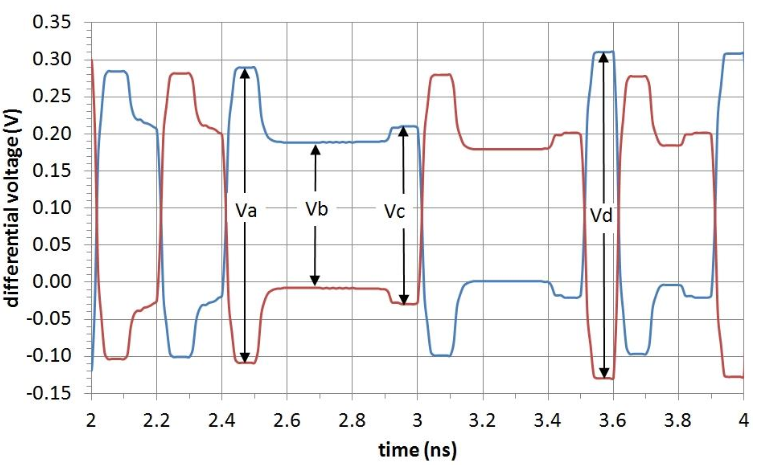
\includegraphics[width=0.8\textwidth]{figures/chapter3/from_USB_spec_output_diff_EQ_example.png}
    \caption{Example output waveform provided in the USB 3.2 specification. Reproduced from \cite{usb32_specs}}
    \label{fig:EQ_example_from_USB_spec}
\end{figure}

Since equalization is defined as a ratio of voltages, each of the output voltages $V_a$, $V_b$ and $V_c$ can be expressed as a function of the equalizer's tap coefficients, $c_{-1}$, $c_0$ and $c_1$, together with the defined output swing, $V_{swing}$:

\begin{align}
V_a &= C_a \cdot V_{swing} = (c_{-1} + c_0 - c_1)\, V_{swing} \\
V_b &= C_b \cdot V_{swing} = (c_{-1} + c_0 + c_1)\, V_{swing} \\
V_c &= C_c \cdot V_{swing} = (-c_{-1} + c_0 + c_1)\, V_{swing}
\label{eq:tap_voltages}
\end{align}

Substituting these expressions into Equation~\eqref{eq:ps_de_definition}, the \ac{PS} and \ac{DE} ratios can be written directly in terms of the tap coefficients, as shown in Equation~\eqref{eq:tap_coefficients}:

\begin{equation}
PS\,(\mathrm{dB}) = 20\log\left(\frac{-c_{-1}+c_0+c_1}{c_{-1}+c_0+c_1}\right), \qquad
DE\,(\mathrm{dB}) = 20\log\left(\frac{c_{-1}+c_0+c_1}{c_{-1}+c_0-c_1}\right)
\label{eq:tap_coefficients}
\end{equation}

The output swing itself is set by the difference between $V_{DD}$ and $V_{DD} - R I_{SS}/2$, so that $V_{swing} = R I_{SS}/2$. Substituting this into the expressions for $V_a$, $V_b$ and $V_c$ gives

\begin{align}
V_a &= (c_{-1} + c_0 - c_1)\,\frac{R I_{SS}}{2} = c_{-1}\frac{R I_{SS}}{2} + c_0\frac{R I_{SS}}{2} - c_1\frac{R I_{SS}}{2} \\
V_b &= (c_{-1} + c_0 + c_1)\,\frac{R I_{SS}}{2} = c_{-1}\frac{R I_{SS}}{2} + c_0\frac{R I_{SS}}{2} + c_1\frac{R I_{SS}}{2} \\
V_c &= (-c_{-1} + c_0 + c_1)\,\frac{R I_{SS}}{2} = -c_{-1}\frac{R I_{SS}}{2} + c_0\frac{R I_{SS}}{2} + c_1\frac{R I_{SS}}{2}
\end{align}

This decomposition shows that the termination current pulled by each tap can be expressed as the product of that tap's coefficient and the termination current $I_{SS}/2$, as shown in Equation~\eqref{eq:tap_current}:

\begin{equation}
I_{c_{-1}} = c_{-1}\,\frac{I_{SS}}{2}, \qquad I_{c_0} = c_0\,\frac{I_{SS}}{2}, \qquad I_{c_1} = c_1\,\frac{I_{SS}}{2}
\label{eq:tap_current}
\end{equation}

\begin{figure}[h]
    \centering
    \begin{tikzpicture}[scale=0.8, transform shape]
        % Paths, nodes and wires:
        \draw (0, 4) -- (0, 0) -- (3, 2) -- (0, 4);
        \draw (11, 4) -- (11, 0) -- (14, 2) -- (11, 4);
        \draw (1.5, 3) to[short] (11, 3);
        \draw (1.5, 1) to[short] (11, 1);
        \node[shape=circle, fill={rgb,255:red,0;green,0;blue,0}, draw, line width=1pt, minimum width=0.215cm] at (1.5, 3){};
        \draw (10, 6) to[american resistor, -*] (10, 3);
        \draw (8.75, 6) to[american resistor] (8.75, 3);
        \draw (5.75, 6) to[american resistor, -*] (5.75, 3);
        \draw (4.5, 6) to[american resistor] (4.5, 3);
        \draw (4.5, 3) to[short, -*] (4.5, 1);
        \draw (8.75, 3) to[short, -*] (8.75, 1);
        \node[vcc] at (4.5, 6){};
        \node[vcc] at (5.75, 6){};
        \node[vcc] at (8.75, 6){};
        \node[vcc] at (10, 6){};
        \node[shape=rectangle, minimum width=1.465cm, minimum height=0.965cm] at (1, 2){} node[anchor=center, align=center, text width=1.077cm, inner sep=6pt] at (1, 2){\huge TX};
        \node[shape=rectangle, minimum width=1.465cm, minimum height=0.965cm] at (12, 2){} node[anchor=center, align=center, text width=1.077cm, inner sep=6pt] at (12, 2){\huge RX};
        \draw[line width=0.9pt, -latex] (6.25, 5.25) -- (6.25, 4);
        \draw[line width=0.9pt, -latex] (10.5, 5.25) -- (10.5, 4);
        \node[shape=rectangle, minimum width=0.715cm, minimum height=0.715cm] at (6.75, 4.625){} node[anchor=center, align=center, text width=0.327cm, inner sep=6pt] at (6.75, 4.625){\Large $I_1$};
        \node[shape=rectangle, minimum width=0.715cm, minimum height=0.715cm] at (11, 4.625){} node[anchor=center, align=center, text width=0.327cm, inner sep=6pt] at (11, 4.625){\Large $I_2$};
        \draw[line width=0.9pt, -latex] (3.75, 3.125) -- (2.5, 3.125);
        \node[shape=rectangle, minimum width=1.965cm, minimum height=0.715cm] at (3.25, 3.5){} node[anchor=center, align=center, text width=1.577cm, inner sep=6pt] at (3.25, 3.5){\Large $I_1 + I_2$};
    \end{tikzpicture}
    \caption{\ac{TX} and \ac{RX} termination currents} \label{fig:tx_rx_termination}
\end{figure}

Furthermore, since each tap must sink the current required to generate the voltage swing across both the \ac{TX} and \ac{RX} terminations, as seen in Figure~\ref{fig:tx_rx_termination}, its tail current is twice the corresponding termination current, as given in Equation~\eqref{eq:tap_tail_current}:

\begin{equation}
I_{tail,\,c_{-1}} = 2 I_{c_{-1}} = c_{-1} I_{SS}, \qquad
I_{tail,\,c_0} = 2 I_{c_0} = c_0 I_{SS}, \qquad
I_{tail,\,c_1} = 2 I_{c_1} = c_1 I_{SS}
\label{eq:tap_tail_current}
\end{equation}

By defining fixed equalization presets, and consequently fixed tap coefficients, the current that each tap must sink to achieve the desired equalization can therefore be calculated directly from Equations~\eqref{eq:tap_current} and~\eqref{eq:tap_tail_current}. It should be noted that the tap coefficients are not independent, but must satisfy the normalization constraint

\begin{equation}
|c_{-1}| + |c_0| + |c_1| = 1
\label{eq:tap_constraint}
\end{equation}

which ensures that the sum of the absolute values of the coefficients remains equal to unity for all valid equalization presets, or, in current terms, that the total current sunk by the driver remains constant regardless of the equalization setting applied.

\subsection{Equalization Settings}

With the relationships between the equalization coefficients and the current sunk by each tap established, the next step is to determine the specific values of the coefficients corresponding to the equalization presets. The \ac{USB} 3.2 specification does not provide explicit values for the coefficients, but rather a interval of \ac{PS} and \ac{DE} values, from which the coefficients can be arbitrarily defined with respect to the constraint defined in Equation~\eqref{eq:tap_constraint}. 

\begin{figure}[h]
	\centering
	\begin{tikzpicture}[transform shape]
		% Paths, nodes and wires:
		\node[shape=rectangle, draw, line width=1pt, minimum width=1.965cm, minimum height=2.965cm] at (1.25, 1.5){} node[anchor=center, align=center, text width=1.577cm, inner sep=6pt] at (1.25, 1.5){TAP\\UNIT\\<0>};
		\draw (0.625, 3) to[short, -*] (0.625, 4.5);
		\node[shape=rectangle, draw, line width=1pt, minimum width=1.965cm, minimum height=2.965cm] at (4.25, 1.5){} node[anchor=center, align=center, text width=1.577cm, inner sep=6pt] at (4.25, 1.5){TAP\\UNIT\\<1>};
		\node[shape=rectangle, draw, line width=1pt, minimum width=1.965cm, minimum height=2.965cm] at (9.25, 1.5){} node[anchor=center, align=center, text width=1.577cm, inner sep=6pt] at (9.25, 1.5){TAP\\UNIT\\<N>};
		\draw (1.875, 3) to[short, -*] (1.875, 3.875);
		\draw[-latex] (0.75, 3.625) -- (0.75, 3.125);
		\node[shape=rectangle, minimum width=0.34cm, minimum height=0.34cm] at (0.938, 3.437){} node[anchor=center, align=center, text width=-0.048cm, inner sep=6pt] at (0.938, 3.437){\footnotesize $\mathrm{I_0}$};
		\draw (3.625, 3) to[short, -*] (3.625, 4.5);
		\draw (4.875, 3) to[short, -*] (4.875, 3.875);
		\draw[-latex] (3.75, 3.625) -- (3.75, 3.125);
		\node[shape=rectangle, minimum width=0.34cm, minimum height=0.34cm] at (3.937, 3.437){} node[anchor=center, align=center, text width=-0.048cm, inner sep=6pt] at (3.937, 3.437){\footnotesize $\mathrm{I_1}$};
		\draw (8.625, 3) to[short, -*] (8.625, 4.5);
		\draw (9.875, 3) to[short, -*] (9.875, 3.875);
		\draw[-latex] (8.75, 3.625) -- (8.75, 3.125);
		\node[shape=rectangle, minimum width=0.34cm, minimum height=0.34cm] at (8.937, 3.437){} node[anchor=center, align=center, text width=-0.048cm, inner sep=6pt] at (8.937, 3.437){\footnotesize $\mathrm{I_N}$};
		\draw (-0, 4.5) -- (10.25, 4.5);
		\draw (10.25, 3.875) -- (-0, 3.875);
		\node[shape=rectangle, minimum width=1.965cm, minimum height=1.09cm] at (6.625, 1.688){} node[anchor=center, align=center, text width=1.577cm, inner sep=6pt] at (6.625, 1.688){\Huge . . .};
		\draw[-latex] (10.125, 4.625) -- (9.25, 4.625);
		\node[shape=rectangle, minimum width=0.34cm, minimum height=0.34cm] at (9.687, 4.875){} node[anchor=center, align=center, text width=-0.048cm, inner sep=6pt] at (9.687, 4.875){\footnotesize $\mathrm{I_{tap}}$};
	\end{tikzpicture}
	\caption{Tap current flow}\label{fig:tap_curr_control}
\end{figure}

The total current sunk by a tap is configured by setting the enable signals of each individual tap unit that composes it. Each tap unit has 6 controllable current mirrors in parallel, each biased to sink a fixed current of 200 $\mathrm{\mu A}$. This structure is what allows each tap to sink a maximum current of 1.2 mA and be digitally controlled in steps of 200 $\mathrm{\mu A}$. The current sunk by each tap is therefore given by the sum of the currents sunk by each of its active tap units, as shown in Figure~\ref{fig:tap_curr_control}. The total current sunk by a tap is therefore given by

\begin{equation}
I_{tap} = I_{mirror} \cdot \sum_{i=0}^{N} \sum_{j=0}^{5} en_{ij} 
\end{equation}

where $en_{ij}$ is the boolean value, '0' or '1', of the enable signal of current mirror $j$ in tap unit $i$, and $I_{mirror}$ is the current sunk by each active current mirror. 

The minimum number of tap units per tap is determined by the maximum current that tap must sink to achieve the defined equalization settings.

\subsubsection{Equalization Presets and Current Requirements} \label{sec:eq_presets_current}

Table~\ref{tab:equalization_presets} lists the \ac{PS} and \ac{DE} values for each equalization preset, along with the corresponding tap coefficients and tap currents calculated according to the relationships defined by Equation~\eqref{eq:tap_tail_current}.

\begin{center}
	\captionof{table}{Equalization Presets}\label{tab:equalization_presets}
	\begin{tabular}{ccccccccc}
		\hline \hline	
		\textbf{Preset} & \textbf{PS (dB)} & \textbf{DE (dB)} & \textbf{$\mathrm{c_{-1}}$} & \textbf{$\mathrm{c_0}$} & \textbf{$\mathrm{c_1}$} & \textbf{$\mathrm{I_{pre}}$ (mA)} & \textbf{$\mathrm{I_{main}}$ (mA)} & \textbf{$\mathrm{I_{post}}$ (mA)}\\
		\hline
		EQ0 & 0 & 0 & 0 & 1 & 0 & 0 & 24 & 0 \\
		EQ1 & 1.2 & 2.1 & -0.052 & 0.852 & -0.096 & 1.25 & 20.4 & 2.3 \\
		EQ2 & 2.2 & 3.1 & -0.084 & 0.791 & -0.125 & 2.02 & 19.0 & 3.0 \\
		EQ3 & 3.2 & 7 & -0.083 & 0.686 & -0.231 & 1.99 & 16.5 & 5.54 \\
		EQ4 & 2.5 & 5 & -0.079 & 0.737 & -0.184 & 1.90 & 17.7 & 4.42 \\
		\hline \hline
	\end{tabular}
\end{center}

With the equalization presets chosen, the corresponding tap coefficients can be calculated using the following equations

\begin{center}
\begin{align}
	k = 10^{PS/20},
	l = 10^{-DE/20} \\
	C_{-1} = \frac{l \times (1-k)}{2 \times (k\times l + 1 - l)} \\
	C_1 = \frac{l - 1}{2 \times (k\times l + 1 - l)} \\
	C_0 = 1 - abs(C_{-1}) - abs(C_1)
\end{align}
\end{center}

The \ac{USB} specification reports de-emphasis as a positive magnitude. Accordingly, $DE_{\mathrm{mag}}$ is used throughout this work. The quantity $l$ represents the ratio $V_b/V_a$, which is smaller than unity for de-emphasized steady-state symbols; therefore, $l=10^{-DE_{\mathrm{mag}}/20}$.

The maximum current that each tap is expected to sink in order to achieve all the desired presets can be calculated, along with the number of tap units required to sink that current. With a tap unit being capable of sinking a maximum current of 1.2 mA, the minimum number of tap units required for each tap can be calculated by

\begin{equation}
	N_{tap} = \left\lceil \frac{I_{tap,max}}{I_{unit}} \right\rceil
\end{equation}

where $I_{tap,max}$ is the maximum current that the tap must sink to achieve the desired equalization range, and $I_{unit}$ is the maximum current that a single tap unit can sink, with the minimum number of tap units required being the ceiling of the ratio between these two values.

From this calculation, the minimum implementation requires 20 tap units for the main tap, 2 for the pre-cursor tap, and 6 for the post-cursor tap. This corresponds to minimum current-control capacities of 120, 12, and 36 enable signals, respectively. As discussed in Section~\ref{sec:overall_driver_architecture}, the final main-cursor stage was expanded from 20 to 24 tap units, increasing its available current-mirror segments from 120 to 144. Table~\ref{tab:eq_enable_map} lists the number of enabled segments required for the nominal equalization presets; the additional 24 main-tap segments remain available as tuning margin.

Because the current banks have a resolution of 200~\textmu A, the analytical current targets in Table~\ref{tab:equalization_presets} cannot in general be realised exactly. The enable counts in Table~\ref{tab:eq_enable_map} therefore correspond to the nearest practical current allocation used as the initial configuration for circuit-level verification.

\begin{center}
	\captionof{table}{Enable Signal Mapping}\label{tab:eq_enable_map}
	\begin{tabular}{cccc}
		\hline \hline	
		\textbf{Preset} & \textbf{\# $\mathrm{en_{pre}}$} & \textbf{\# $\mathrm{en_{main}}$} & \textbf{\# $\mathrm{en_{post}}$} \\
		\hline
		EQ0 & 0 & 120 & 0 \\
		EQ1 & 7 & 102 & 12 \\
		EQ2 & 10 & 95 & 15 \\
		EQ3 & 10 & 83 & 28 \\
		EQ4 & 10 & 89 & 22 \\
		\hline \hline
	\end{tabular}
\end{center}

\begin{comment}
    - The USB 3.2 specifies the transmitter equalization settings as a range
    - Preshoot has a min of 1.2 dB and max of 3.2 dB
    - De-emphasis has a min of -7 dB and a max of -2.1 dB
    - Preshoot and de-emphasis are defined as ratios of the differential output voltage at different instants of the transmitted waveform
    - PS(dB) = 20log(Vc/Vb) and DE(dB) = 20log(Vb/Va)
    - With equalization being defined a ratio of voltages, each output voltage, Va, Vb and Vc, can be expressed as a function of the taps' coefficients, c-1, c0 and c1, and the defined output swing, Vswing
    - Va = Ca * Vswing = (c-1 + c0 - c1) * Vswing; Vb = Cb * Vswing = (c-1 + c0 + c1) * Vswing; Vc = Cc * Vswing = (-c-1 + c0 + c1) * Vswing
    - Voltage ratios can be defined by the coefficients of the taps, as shown in Equation~\ref{eq:tap_coefficients}. (PS=20log((-c-1+c0+c1)/(c-1+c0+c1)) and DE=20log((c-1+c0+c1)/(c-1+c0-c1)))
    - The output swing is between VDD and VDD - RIss/2, so Vswing = RIss/2
    - Va = (c-1 + c0 - c1) * RIss/2 = c-1 * RIss/2 + c0 * RIss/2 - c1 * RIss/2 ; Vb = (c-1 + c0 + c1) * RIss/2 = c-1 * RIss/2 + c0 * RIss/2 + c1 * RIss/2 ; Vc = (-c-1 + c0 + c1) * RIss/2 = -c-1 * RIss/2 + c0 * RIss/2 + c1 * RIss/2
    - This means that the termination current pulled by each tap can be expressed as the product of the tap's coefficient and the termination current, I$_{SS}$/2, as shown in Equation~\ref{eq:tap_current}.
    - Since each tap sinks the current needed to generate the swing on both the TX and RX termination, its tail current is double the termination current, as shown in Equation~\ref{eq:tap_tail_current}.
    - By defining fixed equalization presets, and, by consequence, defined tap coefficients, the current that each tap needs to sink in order to achieve the desired equalization can be calculated
    - Tap coefficients need to satisfy equation |c-1| + |c0| + |c1| = 1, so the sum of the absolute values of the coefficients is equal to 1
\end{comment}

\begin{comment} 
- USB 3.2 Gen 2 specification requires a transmitter equalization to compensate for the channel loss at high frequencies
- Equalization is implemented using a feed-forward equalizer (FFE) in the transmitter, following a 3-tap Finite Impulse Response (FIR) filter structure
- Equalization performs preshoot and de-emphasis
- Preshoot and de-emphasis are functionally set by the FIR filter coefficients
- In practice, preshoot and de-emphasis are measured as the ratio between the differential output voltage at different times of transmission
- Since the USB specification defines a nominal value of 100 ohms for the differential load, the output voltage can be expressed as a function of the load resistance and the tail current, as shown in Equation~\ref{eq:vout_functional}. This way, the preshoot and de-emphasis can be set by controlling the tail current
\end{comment}

\section{Driver Implementation} \label{sec:driver_implementation}

\subsection{Tap Unit}

\begin{comment}
    - Each segment, or tap unit, is composed of a differential pair with a current mirror bank
    - The current mirror bank acts as the tunable current source, and is composed of 6 current mirrors, each paired with a NMOS that acts as a switch to turn on/off each current mirror
    - Each tap unit has two 1k resistors, one for each output, and when combined with the other tap units, they form the tunable termination of the driver
\end{comment}

The driver is implemented as a segmented, current-mode structure in which each of the three FIR taps described in the previous section is realised by an array of identical physical tap units. Each tap unit is composed of a differential pair together with a six-segment current-mirror bank and contributes a digitally controllable fraction of the total tap current. Because the pre-cursor, main-cursor, and post-cursor stages are realised as separate, independently sized and independently enabled arrays of tap units, the driver as a whole implements the FIR summation of Equation~\eqref{eq:fir_3tap} directly in the current domain. The corresponding tap-unit schematic, including the differential pair, switchable current mirrors, and local termination elements, is shown in Figure~\ref{fig:tap_unit_schematic}.

\begin{figure}[H]
    \centering
	\begin{tikzpicture}[scale=0.8, transform shape]
		% Paths, nodes and wires:
		\node[shape=rectangle, draw={rgb,255:red,0;green,128;blue,128}, line width=1pt, dash pattern={on 4pt off 4pt}, minimum width=13.798cm, minimum height=4.798cm] at (7, 2.5){} node[anchor=south, align=center, text width=13.41cm, inner sep=6pt] at (7, 0.083){\textcolor{rgb,255:red,0;green,128;blue,128}{Current Mirror Bank}};
		\node[nmos] at (6.25, 6.583){};
		\node[nmos, xscale=-1, yscale=-1] at (7.25, 6.583){};
		\draw (5.27, 6.583) -- (4.77, 6.583);
		\draw (6.25, 5.813) -| (6.25, 5.583) -- (7.25, 5.583) -| (7.25, 5.833);
		\draw (8.23, 6.583) -- (8.25, 6.583) -| (8.25, 5.917) -- (4.75, 5.917);
		\node[nmos] at (2.437, 3.393){};
		\node[nmos] at (2.437, 1.853){};
		\node[shape=rectangle, minimum width=0.965cm, minimum height=0.631cm] at (0.667, 3.417){} node[anchor=center, align=center, text width=0.577cm, inner sep=6pt] at (0.667, 3.417){\small en<0>};
		\node[shape=rectangle, minimum width=0.965cm, minimum height=0.631cm] at (0.917, 1.917){} node[anchor=center, align=center, text width=0.577cm, inner sep=6pt] at (0.917, 1.917){\small $\mathrm{V_{REF}}$};
		\node[nmos] at (4.603, 3.393){};
		\node[nmos] at (4.603, 1.853){};
		\node[shape=rectangle, minimum width=0.965cm, minimum height=0.631cm] at (2.833, 3.417){} node[anchor=center, align=center, text width=0.577cm, inner sep=6pt] at (2.833, 3.417){\small en<1>};
		\node[nmos] at (6.77, 3.393){};
		\node[nmos] at (6.77, 1.853){};
		\node[shape=rectangle, minimum width=0.965cm, minimum height=0.631cm] at (5, 3.417){} node[anchor=center, align=center, text width=0.577cm, inner sep=6pt] at (5, 3.417){\small en<2>};
		\node[nmos] at (8.937, 3.393){};
		\node[nmos] at (8.937, 1.853){};
		\node[shape=rectangle, minimum width=0.965cm, minimum height=0.631cm] at (7.167, 3.417){} node[anchor=center, align=center, text width=0.577cm, inner sep=6pt] at (7.167, 3.417){\small en<3>};
		\node[nmos] at (11.103, 3.393){};
		\node[nmos] at (11.103, 1.853){};
		\node[shape=rectangle, minimum width=0.965cm, minimum height=0.631cm] at (9.333, 3.417){} node[anchor=center, align=center, text width=0.577cm, inner sep=6pt] at (9.333, 3.417){\small en<4>};
		\node[nmos] at (13.27, 3.393){};
		\node[nmos] at (13.27, 1.853){};
		\node[shape=rectangle, minimum width=0.965cm, minimum height=0.631cm] at (11.5, 3.417){} node[anchor=center, align=center, text width=0.577cm, inner sep=6pt] at (11.5, 3.417){\small en<5>};
		\draw (12.29, 1.853) to[short] (1.457, 1.853);
		\draw (2.437, 4.083) -| (2.437, 4.583) -| (13.27, 4.083);
		\draw (4.603, 4.083) to[short, -*] (4.603, 4.583);
		\draw (6.77, 4.083) to[short, -*] (6.77, 4.583);
		\draw (8.937, 4.083) to[short, -*] (8.937, 4.583);
		\draw (11.103, 4.083) to[short, -*] (11.103, 4.583);
		\node[vee] at (2.437, 1.083){};
		\node[vee] at (4.603, 1.083){};
		\node[vee] at (6.77, 1.083){};
		\node[vee] at (8.937, 1.083){};
		\node[vee] at (11.103, 1.083){};
		\node[vee] at (13.27, 1.083){};
		\draw (6.77, 4.583) to[short, *-*] (6.77, 5.583);
		\node[circ] at (4.77, 6.583){};
		\node[circ] at (4.75, 5.917){};
		\draw (6.25, 9.397) to[american resistor, /tikz/circuitikz/bipoles/length=0.980cm] (6.25, 7.897);
		\draw (7.25, 9.397) to[american resistor, /tikz/circuitikz/bipoles/length=0.980cm] (7.25, 7.897);
		\node[pmos] at (6.25, 10.167){};
		\node[pmos, xscale=-1, yscale=-1] at (7.25, 10.167){};
		\node[vcc] at (6.25, 10.937){};
		\node[vcc] at (7.25, 10.937){};
		\draw (7.25, 7.897) -| (7.25, 7.353);
		\draw (6.25, 7.897) -| (6.25, 7.353);
		\node[circ] at (1.457, 3.393){};
		\node[circ] at (3.623, 3.393){};
		\node[circ] at (5.79, 3.393){};
		\node[circ] at (7.957, 3.393){};
		\node[circ] at (10.123, 3.393){};
		\node[circ] at (12.29, 3.393){};
		\node[circ] at (1.457, 1.853){};
		\draw (5.27, 10.167) -- (4.77, 10.167);
		\draw (8.23, 10.167) -- (8.23, 10.167) -| (8.25, 9.583) -- (4.75, 9.583);
		\node[circ] at (4.77, 10.167){};
		\node[circ] at (4.75, 9.583){};
		\node[shape=rectangle, minimum width=1.631cm, minimum height=0.631cm] at (3.937, 10.167){} node[anchor=center, align=center, text width=1.243cm, inner sep=6pt] at (3.937, 10.167){\small en\_termn};
		\node[shape=rectangle, minimum width=1.631cm, minimum height=0.631cm] at (3.917, 9.583){} node[anchor=center, align=center, text width=1.243cm, inner sep=6pt] at (3.917, 9.583){\small en\_termp};
		\node[shape=rectangle, minimum width=0.798cm, minimum height=0.631cm] at (4.333, 6.583){} node[anchor=center, align=center, text width=0.41cm, inner sep=6pt] at (4.333, 6.583){\small $\mathrm{D_p}$};
		\node[shape=rectangle, minimum width=0.798cm, minimum height=0.631cm] at (4.333, 5.917){} node[anchor=center, align=center, text width=0.41cm, inner sep=6pt] at (4.333, 5.917){\small $\mathrm{D_n}$};
		\draw (6.25, 7.75) to[short, *-*] (9.25, 7.75);
		\draw (7.25, 7.25) to[short, *-*] (9.25, 7.25);
		\node[shape=rectangle, minimum width=0.798cm, minimum height=0.631cm] at (9.667, 7.75){} node[anchor=center, align=center, text width=0.41cm, inner sep=6pt] at (9.667, 7.75){\small $\mathrm{TX_n}$};
		\node[shape=rectangle, minimum width=0.798cm, minimum height=0.631cm] at (9.667, 7.25){} node[anchor=center, align=center, text width=0.41cm, inner sep=6pt] at (9.667, 7.25){\small $\mathrm{TX_p}$};
		\node[shape=rectangle, draw={rgb,255:red,255;green,0;blue,0}, line width=1pt, dash pattern={on 4pt off 4pt}, minimum width=3.631cm, minimum height=4.131cm] at (6.917, 10){} node[anchor=north, align=center, text width=3.243cm, inner sep=6pt] at (6.917, 12.083){\textcolor{rgb,255:red,255;green,0;blue,0}{Termination Control}};
	\end{tikzpicture}
	\caption{Tap unit schematic}\label{fig:tap_unit_schematic}
\end{figure}

Within each tap unit, the current mirror bank acts as the tunable current source and is composed of six current mirrors, each paired with an NMOS device that acts as a switch to enable or disable that mirror. This segmentation allows  the current steered by the differential pair to be adjusted digitally by enabling or disabling individual mirrors, rather than through a continuously variable bias. In addition to the current mirror bank, each tap unit incorporates two 1\,k$\Omega$ resistors, one associated with each of the differential outputs. These resistors are not specific to any single tap; rather, when the resistors from all three taps are combined in parallel, they form the tunable termination network of the driver as a whole. This co-location of the termination resistors within each tap unit allows the termination to be adjusted using the same segmented, switch-based approach used for the current sources, and keeps the layout of each tap unit self-contained, discussed in Section~\ref{sec:layout}.

\begin{comment}
	- Spec requires a termination of 50 ohms
	- Spec gives Vout range
	- I chose to design for the maximum output swing of 1.2Vpp
	- Vo,diff = 1.2 Vpp means Vo,SE = 0.6 Vpp
	- My Vo = (Vds of the differential pair device turned on) + (Vds of the mirror) have a min value of 0.6V
	- My minimum Id is 200 uA, and my maximum Id is 1.2 mA
	- When a device of the diff pair is on, it must stay in saturation
	- The other device of the differential pair is off, and must stay in cutoff
	- Any active current mirror must stay in saturation
	- My worst case for biasing is when my Id is minimum, 200 uA, and my Vout is minimum, 0.6V
	- Each mirror has a fixed Id of 200uA
	- So my current steering device must be in saturation for a Vout range of 0.6V to 1.2V, and a Id range of 200 uA to 1.2 mA
	- Vds_pair_device = Vd - Vs = Vout - Vs
	- Vgs_pair_device = Vg - Vs = Vin - Vds_mirror
	- Vds_mirror = Vd - VSS = Vout - Vds_pair_device
	- Vgs_mirror = Vg - VSS = Vref
	- Before defining the diff pair device Vov for saturation, the mirror Vov need to be defined
	- Mirror Vov = Vgs - Vth = Vref - Vth
	- Vth is fixed for the process, and Vref is defined by the mirror biasing circuit, so the mirror Vov is fixed
	- Since mirror Vov and Id is equal to the reference transistor, the reference circuit must be designed to provide the desired current
	- After the reference circuit is designed, and the mirror Vov is defined, the diff pair device Vov can be defined to ensure that the diff pair device stays in saturation for the desired Id and Vout range
	- Since the mirror is the same size as the ref device, its Id is fixed at 200 uA, and its Vov is fixed, the diff pair Vs is defined, since it is equal to the mirror Vds
	- With this, the diff pair device Vs is defined, and its sizing can be swept in order to find a Vth that ensures saturation, that is, Vds > Vov, and the Vg, or Vin, can be swept to find the Vgs that ensures saturation, that is, Vgs > Vth, for the worst case of Id = 200 uA and Vout = 0.6V
	- Then the Vin for the off device can be swept to find the Vgs that ensures cutoff
	- With the Vin swing defined, the diff pair must be simulated and validates for the entire range of Id and Vout, to ensure that the diff pair device stays in saturation for the on device, and in cutoff for the off device, for the entire range of Id and Vout
    
\end{comment}

\subsection{Tap Unit Sizing and Biasing}

The \ac{USB} 3.2 specification requires a nominal single-ended termination of 50\,$\Omega$ at each output, and additionally defines an allowable range for the transmitted output voltage swing. Within this range, the driver described in this work was designed to support the maximum specified differential output swing of 1.2\,V\textsubscript{pp}, in order to maximize the control margin of the driver. Since the differential swing is split equally between the two single-ended outputs, a differential swing, $V_{out,diff}$, of $\mathrm{1.2\,V_{pp}}$ corresponds to a single-ended swing of

\begin{equation}
V_{\mathrm{swing,SE}} = \frac{V_{\mathrm{out,diff,pp}}}{2} = 0.6~\mathrm{V_{pp}}.
\label{eq:vo_se}
\end{equation}

at each output node.

%Each output node of the driver settles to a voltage set by the sum of the drain-source voltage of the differential pair device that is turned on, $V_{DS,pair}$, and the drain-source voltage of the current mirror device that steers the corresponding tap current, $V_{DS,mirror}$. 

Each output node of the driver settles to a voltage set by difference between $\mathrm{V_{DD}}$ and the voltage drop across the termination:

\begin{equation}
V_{\mathrm{out,L}} = V_{DD} - \frac{I_{SS}}{2}R_{\mathrm{term}}.
\end{equation}

At the maximum differential output swing, the minimum output-node voltage is therefore approximately 0.6~V. At the same time, the current delivered by each tap unit is not fixed, but is instead digitally programmable, as described in the preceding section, ranging from a minimum drain current of $I_{D,min} = 200\,\mathrm{\mu A}$, corresponding to a single active current mirror, up to a maximum of $I_{D,max} = 1.2\,\mathrm{mA}$, corresponding to all six mirrors active simultaneously.

For correct operation of the driver, three conditions must be satisfied simultaneously, for every combination of output voltage and tap current within the range defined above:

\begin{itemize}
    \item The device of the differential pair that is turned on by the input data must remain in saturation, so that it behaves as a well-defined current source and the tap current is accurately steered to the intended output.
    \item The device of the differential pair that is turned off must remain in cutoff, so that it contributes no current to the opposite output and the full tap current is steered to only one side of the differential output; however, this device should not be driven too deep into cutoff, since doing so would require an unnecessarily large input voltage swing, which in turn would degrade the driver's switching speed.
    \item All active current mirror devices remain in saturation, so that the current sourced by each unit mirror accurately reflects its reference current, independent of the output voltage.
\end{itemize}

% First, whichever device of the differential pair is turned on by the input data must remain in saturation, so that it behaves as a well-defined current source and the tap current is accurately steered to the intended output. 
% Second, the device of the differential pair that is turned off must remain in cutoff, so that it contributes no current to the opposite output and the full tap current is steered to only one side of the differential output; however, this device should not be driven too deep into cutoff, since doing so would require an unnecessarily large input voltage swing, which in turn would degrade the driver's switching speed. 
% Third, whichever current mirror devices are active for a given tap setting must themselves remain in saturation, so that the current sourced by each unit mirror accurately reflects its designed value of 200\,\textmu A, independent of the output voltage.

With the output defining the available voltage headroom in which both the active differential pair and active mirror devices must remain in saturation, and the variability of the tap current defining the range of drain currents that must be achieved, keeping all three of these conditions satisfied simultaneously across the full range of output voltage and tap current makes it essential to identify the worst-case biasing condition, and to define the sizing and biasing of the differential pair and current mirror devices around that corner. The relevant device voltages in the current-steering path are identified in Figure~\ref{fig:diff_pair_mirror_node_voltages}.

% Because both the output voltage and the tap current are variable, and saturation of the differential pair device becomes more difficult as the available drain-source voltage headroom decreases, the worst-case biasing condition for the differential pair occurs at the lower bound of both ranges simultaneously: a drain current of $I_D = 200\,\mathrm{\mu A}$ and an output voltage of $V_{out} = 0.6\,\mathrm{V}$. It is this corner that the sizing and biasing methodology described in the remainder of this section is designed around, on the basis that if saturation can be guaranteed at this worst-case point, the same devices will remain comfortably in saturation for all other combinations of current and output voltage within the specified ranges, up to $V_{out} = 1.2\,\mathrm{V}$ and $I_D = 1.2\,\mathrm{mA}$.

\begin{figure}[H]
	\centering
	\begin{tikzpicture}[transform shape]
	% Paths, nodes and wires:
		\node[nmos](nmos1) at (1.25, 4.02){};
		\node[nmos, xscale=-1, yscale=-1](nmos2) at (3.25, 4.02){};
		\draw ($(nmos2.D) + (0,-0.1)$) to[open, v_=$V_{GS,pair}$] ($(nmos2.G) + (0,-0.1)$);
		\draw ($(nmos2.D) + (-0.1,0)$) to[open, v^=$V_{DS,pair}$] ($(nmos2.S) + (-0.1,0)$);
		\draw (1.25, 3.25) |- (1.75, 3) -- (3.25, 3) -- (3.25, 3.25);
		\node[nmos](nmos3) at (2.25, 1.23){};
		\draw ($(nmos3.S) + (-0.1,0)$) to[open, v^=$V_{GS,mirror}$] ($(nmos3.G) + (-0.1,0)$);
		\draw ($(nmos3.S) + (0.1,0)$) to[open, v_=$V_{DS,mirror}$] ($(nmos3.D) + (0.1,0)$);
		\node[shape=rectangle, minimum width=0.965cm, minimum height=0.631cm] at (0.73, 1.293){} node[anchor=center, align=center, text width=0.577cm, inner sep=6pt] at (0.73, 1.293){\small $V_{ref}$};
		\node[vee] at (2.25, 0.46){};
		\draw (2.25, 2) to[short, -*] (2.25, 3);
		\node[circ] at (0.27, 4.02){};
		\node[circ] at (4.23, 4.02){};
		\draw (1.25, 6.833) to[american resistor, /tikz/circuitikz/bipoles/length=0.980cm] (1.25, 5.333);
		\draw (3.25, 6.833) to[american resistor, /tikz/circuitikz/bipoles/length=0.980cm] (3.25, 5.333);
		\node[vcc] at (1.25, 6.833){};
		\node[vcc] at (3.25, 6.833){};
		\draw (3.25, 5.333) -| (3.25, 4.79);
		\draw (1.25, 5.333) -| (1.25, 4.79);
		%\node[circ] at (1.27, 1.23){} node[anchor=east] at (1.27, 1.23){\small $\mathrm{V_{tail}}$};
		\node[shape=rectangle, minimum width=0.798cm, minimum height=0.631cm] at (4.667, 4){};
		\node[circ] at (1.25, 5.333){};
		\node[circ] at (3.25, 5.333){};
		\node[shape=rectangle, minimum width=0.798cm, minimum height=0.631cm](Vo_p) at (3.667, 5.417){} node[anchor=center, align=center, text width=0.41cm, inner sep=6pt] at (3.667, 5.417){\small $V_{out,P}$};
		\node[shape=rectangle, minimum width=0.798cm, minimum height=0.631cm] at (-0.667, 4){} node[anchor=center, align=center, text width=0.41cm, inner sep=6pt] at (-0.667, 4){\small $V_{in,P}$};
		\node[shape=rectangle, minimum width=0.798cm, minimum height=0.631cm] at (0.417, 5.417){} node[anchor=center, align=center, text width=0.41cm, inner sep=6pt] at (0.417, 5.417){\small $V_{out,N}$};
		\node[flowarrow, rotate=-90](N1) at (2.5, 2.5){} node[anchor=west] at (N1.text){$\mathrm{I_{SS}}$};
		%\node[flowarrow, rotate=-90](N2) at (1.5, 4.75){} node[anchor=west] at (N2.text){$\mathrm{0 A}$};
		%\node[flowarrow, rotate=-90](N3) at (3.5, 4.75){} node[anchor=west] at (N3.text){$\mathrm{200 \mu A}$};
		%\draw ($(nmos3.S) + (3,0)$) to[open, v_=$V_{DS,mirror}$] ($(Vo_low) + (3,0)$);
	\end{tikzpicture}
	\caption{Differential pair and current mirror node voltages}\label{fig:diff_pair_mirror_node_voltages}
\end{figure}

Using a diode connected NMOS circuit to generate the biasing voltage, $V_{ref}$, for a reference current, $I_{ref}$, of 200\,\textmu A, a sweep of the mirror device's length was performed to determine which length would provide a stable current copy across the expected $V_{DS}$ range. The length and finger-count sweeps are combined in Figure~\ref{fig:mirror_id_vs_vds}. Its length-sweep panel, Figure~\ref{fig:mirror_id_vs_vds_var_L}, plots the mirror drain current, $I_{D,mirror}$, against $V_{DS}$ for three different device lengths. The results show that a mirror length of $L_{mirr} = 3 \times L_{min}$ provides the best tradeoff between device size and current-copying stability across the expected range of $V_{DS,mirror}$, and was therefore selected for the current mirror devices within each tap unit.

\begin{comment}
\begin{figure}[H]
	\centering
	\begin{tikzpicture}
		\begin{axis}[
			xlabel={$V_{DS,mirror}$ (V)},
			ylabel={$I_{D,mirror}$ (\textmu A)},  
			minor tick num=1, 
			grid=both,
			legend pos=south east,
		]
			%\addplot table [blue, col sep=comma, x=Vds, y=Id] {plot/Mirror_Id_vs_vtail_nf=30_var_L.csv};
			\addplot table [blue, col sep=comma, x expr={\thisrow{L} == 60 ? \thisrow{Vds} : nan}, y=Id] {plot/Mirror_Id_vs_vtail_nf=30_var_L.csv};
			\addlegendentry{L = $\mathrm{L_{min}}$}
			\addplot table [red, col sep=comma, x expr={\thisrow{L} == 120 ? \thisrow{Vds} : nan}, y=Id] {plot/Mirror_Id_vs_vtail_nf=30_var_L.csv};
			\addlegendentry{L = $\mathrm{2 \times L_{min}}$}
			\addplot table [green, col sep=comma, x expr={\thisrow{L} == 180 ? \thisrow{Vds} : nan}, y=Id] {plot/Mirror_Id_vs_vtail_nf=30_var_L.csv};
			\addlegendentry{L = $\mathrm{3 \times L_{min}}$}
		\end{axis}
	\end{tikzpicture}
	\caption{Mirror $I_{D}$ against $V_{DS}$ for varying device lengths}\label{fig:mirror_id_vs_vds_var_L}
\end{figure}
\end{comment}

\begin{figure}[h]
	\begin{subfigure}[b]{0.49\textwidth}
		\centering
		\resizebox{\linewidth}{!}{
			\begin{tikzpicture}
			\begin{axis}[
				xlabel={$V_{DS,mirror}$ (V)},
				ylabel={$I_{D,mirror}$ (\textmu A)},  
				xmin=0, xmax=0.6,
				minor tick num=1, 
				grid=both,
				legend pos=south east,
				no markers,
				every axis plot/.append style={thick}
			]
				%\addplot table [blue, col sep=comma, x=Vds, y=Id] {plot/Mirror_Id_vs_vtail_nf=30_var_L.csv};
				\addplot table [blue, col sep=comma, x expr={\thisrow{L} == 60 ? \thisrow{Vds} : nan}, y=Id] {plot/Mirror_Id_vs_vtail_nf=30_var_L.csv};
				\addlegendentry{L = $\mathrm{L_{min}}$}
				\addplot table [red, col sep=comma, x expr={\thisrow{L} == 120 ? \thisrow{Vds} : nan}, y=Id] {plot/Mirror_Id_vs_vtail_nf=30_var_L.csv};
				\addlegendentry{L = $\mathrm{2 \times L_{min}}$}
				\addplot table [green, col sep=comma, x expr={\thisrow{L} == 180 ? \thisrow{Vds} : nan}, y=Id] {plot/Mirror_Id_vs_vtail_nf=30_var_L.csv};
				\addlegendentry{L = $\mathrm{3 \times L_{min}}$}
			\end{axis}
		\end{tikzpicture}
		}
		\caption{$I_{D}$ versus $V_{DS}$ for varying lengths}\label{fig:mirror_id_vs_vds_var_L}
	\end{subfigure}
	\begin{subfigure}[b]{0.49\textwidth}
		\centering
		\resizebox{\linewidth}{!}{
			\begin{tikzpicture}
			\begin{axis}[
				xlabel={$V_{DS,mirror}$ (V)},
				ylabel={$I_{D,mirror}$ (\textmu A)},  
				xmin=0, xmax=0.6,
				minor tick num=1, 
				grid=both,
				legend pos=south east,
				no markers,
				every axis plot/.append style={thick}
			]
				%\addplot table [blue, col sep=comma, x=Vds, y=Id] {plot/Mirror_Id_vs_vtail_nf=30_var_L.csv};
				\addplot table [blue, col sep=comma, x expr={\thisrow{nf} == 10 ? \thisrow{Vds_mirror} : nan}, y=Id_mirror] {plot/Mirror_Id_vs_vtail_L=0.18_var_nf.csv};
				\addlegendentry{nf=10}
				\addplot table [red, col sep=comma, x expr={\thisrow{nf} == 20 ? \thisrow{Vds_mirror} : nan}, y=Id_mirror] {plot/Mirror_Id_vs_vtail_L=0.18_var_nf.csv};
				\addlegendentry{nf=20}
				\addplot table [purple, col sep=comma, x expr={\thisrow{nf} == 60 ? \thisrow{Vds_mirror} : nan}, y=Id_mirror] {plot/Mirror_Id_vs_vtail_L=0.18_var_nf.csv};
				\addlegendentry{nf=60}
				\addplot table [brown, col sep=comma, x expr={\thisrow{nf} == 80 ? \thisrow{Vds_mirror} : nan}, y=Id_mirror] {plot/Mirror_Id_vs_vtail_L=0.18_var_nf.csv};
				\addlegendentry{nf=80}
			\end{axis}
			\end{tikzpicture}
		}
		\caption{$I_D$ versus $V_{DS}$ with $L = 3 \times L_{min}$}\label{fig:mirror_id_vs_vds_var_nf}
	\end{subfigure}
	\caption{Mirror $I_D$ versus $V_{DS}$ for varying device lengths and finger counts}\label{fig:mirror_id_vs_vds}
\end{figure}

With the mirror length defined, its finger count was then swept to determine which device width would provide the closest match to $I_{ref}$ for the selected length. Figure~\ref{fig:mirror_id_vs_vds_var_nf} shows the results of this sweep, with $I_{D,mirror}$ plotted against its $V_{DS}$ for four different finger counts. The results show that a mirror finger count of $nf = 60$ provides a good trade-off between current matching and device area, and was therefore selected for the current mirror devices within each tap unit.

\begin{comment}
\begin{figure}[H]
	\centering
	\begin{tikzpicture}
		\begin{axis}[
			xlabel={$V_{DS,mirror}$ (V)},
			ylabel={$I_{D,mirror}$ (\textmu A)},  
			minor tick num=1, 
			grid=both,
			legend pos=south east,
		]
			%\addplot table [blue, col sep=comma, x=Vds, y=Id] {plot/Mirror_Id_vs_vtail_nf=30_var_L.csv};
			\addplot table [blue, col sep=comma, x expr={\thisrow{nf} == 10 ? \thisrow{Vds_mirror} : nan}, y=Id_mirror] {plot/Mirror_Id_vs_vtail_L=0.18_var_nf.csv};
			\addlegendentry{nf=10}
			\addplot table [red, col sep=comma, x expr={\thisrow{nf} == 20 ? \thisrow{Vds_mirror} : nan}, y=Id_mirror] {plot/Mirror_Id_vs_vtail_L=0.18_var_nf.csv};
			\addlegendentry{nf=20}
			\addplot table [purple, col sep=comma, x expr={\thisrow{nf} == 60 ? \thisrow{Vds_mirror} : nan}, y=Id_mirror] {plot/Mirror_Id_vs_vtail_L=0.18_var_nf.csv};
			\addlegendentry{nf=60}
			\addplot table [brown, col sep=comma, x expr={\thisrow{nf} == 80 ? \thisrow{Vds_mirror} : nan}, y=Id_mirror] {plot/Mirror_Id_vs_vtail_L=0.18_var_nf.csv};
			\addlegendentry{nf=80}
		\end{axis}
	\end{tikzpicture}

	\caption{Mirror $I_d$ against $V_{ds}$ for varying device finger counts, with a fixed length of $3 \times L_{min}$}\label{fig:mirror_id_vs_vds_var_nf}
\end{figure}
\end{comment}

The total voltage headroom available for the current-steering path is set by the driver's output voltage, and is shared between the current mirror device and the differential pair device connected in series with it, according to

\begin{equation}
V_{DS,mirr} + V_{DS,pair} = V_{out}.
\label{eq:headroom_split}
\end{equation}

To ensure that the mirror remains in saturation, that is, so it's overdrive voltage, $V_{OV}$, is less than its $V_{DS}$, a \ac{SLVT} device flavor was selected, giving more headroom for the current source devices. The pair's overdrive voltage, $V_{OV,pair}$, is arbitrarily defined based on the device's gm/Id ratio that leads to strong inversion operation. The relationship between $g_m/I_D$ and $V_{OV}$, including the weak-, moderate-, and strong-inversion regions, is illustrated in Figure~\ref{fig:gmid_vs_vov}. 

\begin{figure}[H]
	\centering
	\resizebox{0.5\linewidth}{!}{
	\begin{tikzpicture}
		\begin{axis}[
			ylabel={$\frac{gm}{Id}$},
			xlabel={$V_{OV}$ (V)},
			xmin=-0.5, xmax=0.5, 
			ymin=-1, ymax=31, 
			minor tick num=1,
			grid=both,
			legend pos=south east,
			no markers
		]
			\addplot table [blue, col sep=comma, x=vov, y=gmId] {plot/gmid_vov.csv};
			\addplot [color=red, dashed] coordinates {(-0.05, -5) (-0.05, 35)};
			\addplot [color=red, dashed] coordinates {(0.15, -5) (0.15, 35)};
			\addplot [color=red, dashed] coordinates {(-0.3, 15) (-0.3, 15)} node [above] {WI};
			\addplot [color=red, dashed] coordinates {(0.05, 15) (0.05, 15)} node [above] {MI};
			\addplot [color=red, dashed] coordinates {(0.35, 15) (0.35, 15)} node [above] {SI};
	
		\end{axis}
	\end{tikzpicture}
	}
	\caption{$\frac{gm}{Id}$ versus $V_{OV}$}\label{fig:gmid_vs_vov}
\end{figure}

%A value of $V_{OV,\mathrm{pair}}=0.2$~V was selected as a compromise between transconductance, switching speed, device size, and saturation headroom for the current mirrors. The \ac{RVT} device flavor was retained for the differential pair because of its lower leakage relative to the \ac{SLVT} option, while the resulting saturation margin was verified over the complete current and output-voltage ranges in the subsequent simulations.

A value of $V_{OV,\mathrm{pair}}=0.2$~V was selected as a compromise between transconductance, switching speed, device size, and saturation headroom for the current mirrors. The \ac{RVT} device flavor was retained for the differential pair since the required switching speed could be achieved without resorting to \ac{SLVT} devices. In addition to its lower leakage, the higher threshold voltage reduces residual conduction in the nominally off branch, improving current-steering accuracy and limiting unnecessary static current. The resulting saturation margin and switching performance were verified over the complete current and output-voltage ranges in the subsequent simulations.

With the mirror sizing done, a sweep of the differential pair drain current, $I_{D,pair}$, and tail voltage, $V_{tail}$ against a range of $V_{in,CM}$ was performed for different finger counts. To define a starting $V_{in,CM}$, three design considerations must be taken into account:

\begin{enumerate}
	\item For this $V_{in,CM}$ the current steered by the differential pair must be close to the reference current
	\item At the same time, for the selected $V_{in,CM}$, the tail voltage must be high enough to ensure that the mirror device is in saturation
	\item $V_{in,CM}$ must respect the condition presented in Equation~\eqref{eq:vincm_condition}, which ensures that the condition $V_{DS} \geq V_{OV}$ is met for both current mirror and differential pair devices.
\end{enumerate}

The minimum $V_{in,CM}$ determined in Equation~\eqref{eq:vincm_condition} ensures that the mirror remains in saturation, while the maximum $V_{in,CM}$ ensures that both mirror and differential pair devices remain in saturation.
With these three considerations in mind, a $V_{in,CM}$ can be defined that provides a tradeoff between $I_{D,pair}$ and $V_{tail}$, as well as keeping both devices in their desired regions during differential operation.

\begin{equation}
	V_{GS,pair} + V_{OV,mirror} \leq V_{in,CM} \leq \min(V_{DD} - V_{OUT} + V_{TH,pair},  V_{DD})
\label{eq:vincm_condition}
\end{equation}

\begin{figure}[H]
	\begin{subfigure}[b]{0.49\textwidth}
		\centering
		\resizebox{\linewidth}{!}{
		\begin{tikzpicture}
			\begin{axis}[
				xlabel={$V_{in,CM}$ (V)},
				ylabel={$I_{D,pair,N}, I_{D,pair,P}$ (\textmu A)},  
				xmin=0, xmax=1.2, 
				minor tick num=1, 
				grid=both,
				legend pos=south east,
				no markers,
				every axis plot/.append style={thick}
			]
				%\addplot table [blue, col sep=comma, x=vcm, y=idTXp] {plot/diff_pair_vds_id_vtail_vcmin_vcmout.csv};
				\addplot table [blue, col sep=comma, x expr={\thisrow{nf} == 10 ? \thisrow{vcm} : nan}, y=idTXp] {plot/diff_pair_vincm2.csv};
				\addlegendentry{nf=10}
				%\addplot table [red, col sep=comma, x expr={\thisrow{nf} == 20 ? \thisrow{vcm} : nan}, y=idTXp] {plot/diff_pair_vincm2.csv};
				%\addlegendentry{nf=20}
				\addplot table [purple, col sep=comma, x expr={\thisrow{nf} == 30 ? \thisrow{vcm} : nan}, y=idTXp] {plot/diff_pair_vincm2.csv};
				\addlegendentry{nf=30}
				\addplot table [brown, col sep=comma, x expr={\thisrow{nf} == 40 ? \thisrow{vcm} : nan}, y=idTXp] {plot/diff_pair_vincm2.csv};
				\addlegendentry{nf=40}
				\addplot table [orange, col sep=comma, x expr={\thisrow{nf} == 50 ? \thisrow{vcm} : nan}, y=idTXp] {plot/diff_pair_vincm2.csv};
				\addlegendentry{nf=50}
			\end{axis}
		\end{tikzpicture}
		}
		\caption{$I_{D}$ versus $V_{in,CM}$}\label{fig:diff_pair_id_vs_vincm}
	\end{subfigure}
	\begin{subfigure}{0.49\textwidth}
		\centering
		\resizebox{\linewidth}{!}{
		\begin{tikzpicture}
			\begin{axis}[
				xlabel={$V_{in,CM}$ (V)},
				ylabel={$V_{tail}$ (V)}, 
				xmin=0, xmax=1.2, 
				minor tick num=1, 
				grid=both,
				legend pos=north west,
				no markers,
				every axis plot/.append style={thick}
			]
				%\addplot table [blue, col sep=comma, x=vcm, y=vtail] {plot/diff_pair_vds_id_vtail_vcmin_vcmout.csv};
				\addplot table [blue, col sep=comma, x expr={\thisrow{nf} == 10 ? \thisrow{vcm} : nan}, y=vtail] {plot/diff_pair_vincm2.csv};
				\addlegendentry{nf=10}
				%\addplot table [red, col sep=comma, x expr={\thisrow{nf} == 20 ? \thisrow{vcm} : nan}, y=vtail] {plot/diff_pair_vincm2.csv};
				%\addlegendentry{nf=20}
				\addplot table [purple, col sep=comma, x expr={\thisrow{nf} == 30 ? \thisrow{vcm} : nan}, y=vtail] {plot/diff_pair_vincm2.csv};
				\addlegendentry{nf=30}
				\addplot table [brown, col sep=comma, x expr={\thisrow{nf} == 40 ? \thisrow{vcm} : nan}, y=vtail] {plot/diff_pair_vincm2.csv};
				\addlegendentry{nf=40}
				\addplot table [orange, col sep=comma, x expr={\thisrow{nf} == 50 ? \thisrow{vcm} : nan}, y=vtail] {plot/diff_pair_vincm2.csv};
				\addlegendentry{nf=50}
			\end{axis}
		\end{tikzpicture}
		}
		\caption{$V_{tail}$ versus $V_{in,CM}$}\label{fig:diff_pair_vtail_vs_vincm}
	\end{subfigure}
	\begin{subfigure}{0.49\textwidth}
		\centering
		\resizebox{\linewidth}{!}{
		\begin{tikzpicture}
			\begin{axis}[
				xlabel={$V_{in,CM}$ (V)},
				ylabel={$V_{DS}$ (V)},  
				xmin=0, xmax=1.2,
				minor tick num=1, 
				grid=both,
				legend pos=south west,
				no markers,
				every axis plot/.append style={thick}
			]
				%\addplot table [blue, col sep=comma, x=vcm, y=vdsMNP] {plot/diff_pair_vds_id_vtail_vcmin_vcmout.csv};
				\addplot table [blue, col sep=comma, x expr={\thisrow{nf} == 10 ? \thisrow{vcm} : nan}, y=vdsMNp] {plot/diff_pair_vincm2.csv};
				\addlegendentry{nf=10}
				%\addplot table [red, col sep=comma, x expr={\thisrow{nf} == 20 ? \thisrow{vcm} : nan}, y=vdsMNp] {plot/diff_pair_vincm2.csv};
				%\addlegendentry{nf=20}
				\addplot table [purple, col sep=comma, x expr={\thisrow{nf} == 30 ? \thisrow{vcm} : nan}, y=vdsMNp] {plot/diff_pair_vincm2.csv};
				\addlegendentry{nf=30}
				\addplot table [brown, col sep=comma, x expr={\thisrow{nf} == 40 ? \thisrow{vcm} : nan}, y=vdsMNp] {plot/diff_pair_vincm2.csv};
				\addlegendentry{nf=40}
				\addplot table [orange, col sep=comma, x expr={\thisrow{nf} == 50 ? \thisrow{vcm} : nan}, y=vdsMNp] {plot/diff_pair_vincm2.csv};
				\addlegendentry{nf=50}
			\end{axis}
		\end{tikzpicture}
		}
		\caption{$V_{DS}$ versus $V_{in,CM}$}\label{fig:diff_pair_vds_vs_vincm}
	\end{subfigure}
	\caption{Differential pair $I_{D}$, $V_{DS,mirror}$ and $V_{tail}$ versus $V_{in,CM}$ for varying device finger counts}\label{fig:diff_pair_id_vout_vs_vincm}
\end{figure}

The sweeps in Figure~\ref{fig:diff_pair_id_vout_vs_vincm} show how the differential-pair current and internal node voltages vary with input common-mode voltage for different device finger counts. These results support the selection of an initial common-mode bias before the maximum-current corner is evaluated.

Even though this first design corner is a good start for the differential pair design, another issue arises for the case when the tap unit sinks its maximum current. 
With the increase of the tail current, $V_{DS}$ of the steering device increases, while $V_{DS}$ of the mirror device decreases. This leads to a higher $V_{GS}$ on the steering device, increasing its $V_{OV}$ and, if not carefully considered, can lead to the steering device leaving saturation since $V_{DS}$ does not increase at the same rate of increase as $V_{GS}$. This is a corner case that must be considered, and the sizing of the differential pair must be done in a way that ensures that the steering device remains in saturation for the entire current range. This is done by analyzing the system behavior for input swing and maximum current.

By sweeping the differential input voltage around the previously defined $V_{in,CM}$, the current-steering characteristic of the differential pair can be evaluated and an appropriate input swing can be selected. The two input voltages are defined as

\begin{equation}
    V_{in,P}=V_{in,CM}+\Delta
\end{equation}

and

\begin{equation}
    V_{in,N}=V_{in,CM}-\Delta,
\end{equation}

where $\Delta$ represents the voltage excursion of each input from the common-mode level. Therefore, the instantaneous differential input voltage is

\begin{equation}
    V_{IN,diff}=V_{in,P}-V_{in,N}=2\Delta.
\end{equation}

For the opposite logic state, the polarity is reversed, such that $V_{IN,diff}=-2\Delta$. Thus, a value of $\Delta=0.2$~V corresponds to input levels of $1.0$~V and $0.6$~V for $V_{in,CM}=0.8$~V, giving $V_{IN,diff}=\pm0.4$~V, or $0.8$~V$_{pp}$ differential.

\begin{comment}
\begin{figure}[H]
	\begin{subfigure}[b]{0.49\textwidth}
		\centering
		\resizebox{\linewidth}{!}{
		\begin{tikzpicture}
			\begin{axis}[
				xlabel={en},
				xmin=0, xmax=6,
				ylabel={$I_{D,on}$ (\textmu A)},  
				minor tick num=1, 
				grid=both,
				legend pos=north west,
				no markers,
				every axis plot/.append style={thick}
			]
				%\addplot table [blue, col sep=comma, x=vcm, y=idTXp] {plot/diff_pair_vds_id_vtail_vcmin_vcmout.csv};
				%\addplot table [blue, col sep=comma, x expr={\thisrow{delta} == 0 ? \thisrow{en_mirror} : nan}, y=id_pair_n] {plot/Diff_pair_SF_ref2.csv};
				%\addlegendentry{d=0}
				%\addplot table [red, col sep=comma, x expr={\thisrow{delta} == 0.05 ? \thisrow{en_mirror} : nan}, y=id_pair_n] {plot/Diff_pair_SF_ref2.csv};
				%\addlegendentry{d=0.05}
				\addplot table [blue, col sep=comma, x expr={\thisrow{delta} == 0.1 ? \thisrow{en_mirror} : nan}, y=id_pair_n] {plot/Diff_pair_SF_ref2.csv};
				\addlegendentry{$\mathrm{\Delta}$=0.1}
				%\addplot table [brown, col sep=comma, x expr={\thisrow{delta} == 0.15 ? \thisrow{en_mirror} : nan}, y=id_pair_n] {plot/Diff_pair_SF_ref2.csv};
				%\addlegendentry{d=0.15}
				\addplot table [red, col sep=comma, x expr={\thisrow{delta} == 0.2 ? \thisrow{en_mirror} : nan}, y=id_pair_n] {plot/Diff_pair_SF_ref2.csv};
				\addlegendentry{$\mathrm{\Delta}$=0.2}
				%\addplot table [orange, col sep=comma, x expr={\thisrow{delta} == 0.25 ? \thisrow{en_mirror} : nan}, y=id_pair_n] {plot/Diff_pair_SF_ref2.csv};
				%\addlegendentry{d=0.25}
				\addplot table [green, col sep=comma, x expr={\thisrow{delta} == 0.3 ? \thisrow{en_mirror} : nan}, y=id_pair_n] {plot/Diff_pair_SF_ref2.csv};
				\addlegendentry{$\mathrm{\Delta}$=0.3}
				%\addplot table [orange, col sep=comma, x expr={\thisrow{delta} == 0.35 ? \thisrow{en_mirror} : nan}, y=id_pair_n] {plot/Diff_pair_SF_ref2.csv};
				%\addlegendentry{d=0.35}
				\addplot table [orange, col sep=comma, x expr={\thisrow{delta} == 0.4 ? \thisrow{en_mirror} : nan}, y=id_pair_n] {plot/Diff_pair_SF_ref2.csv};
				\addlegendentry{$\mathrm{\Delta}$=0.4}
				%\addplot table [orange, col sep=comma, x expr={\thisrow{delta} == 0.45 ? \thisrow{en_mirror} : nan}, y=id_pair_n] {plot/Diff_pair_SF_ref2.csv};
				%\addlegendentry{d=0.45}
				%\addplot table [orange, col sep=comma, x expr={\thisrow{delta} == 0.5 ? \thisrow{en_mirror} : nan}, y=id_pair_n] {plot/Diff_pair_SF_ref2.csv};
				%\addlegendentry{d=0.5}
			\end{axis}
		\end{tikzpicture}
		}
		\caption{$I_{D,on}$ for input swing}%\label{fig:diff_pair_id_vs_vincm}
	\end{subfigure}
	\begin{subfigure}{0.49\textwidth}
		\centering
		\resizebox{\linewidth}{!}{
		\begin{tikzpicture}
			\begin{axis}[
				xlabel={en},
				xmin=0, xmax=6,
				ylabel={$I_{D,off}$ (\textmu A)},  
				minor tick num=1, 
				grid=both,
				legend pos=north west,
				no markers,
				every axis plot/.append style={thick}
			]
				%\addplot table [blue, col sep=comma, x=vcm, y=idTXp] {plot/diff_pair_vds_id_vtail_vcmin_vcmout.csv};
				%\addplot table [blue, col sep=comma, x expr={\thisrow{delta} == 0 ? \thisrow{en_mirror} : nan}, y=id_pair_p] {plot/Diff_pair_SF_ref2.csv};
				%\addlegendentry{d=0}
				%\addplot table [red, col sep=comma, x expr={\thisrow{delta} == 0.05 ? \thisrow{en_mirror} : nan}, y=id_pair_p] {plot/Diff_pair_SF_ref2.csv};
				%\addlegendentry{d=0.05}
				\addplot table [blue, col sep=comma, x expr={\thisrow{delta} == 0.1 ? \thisrow{en_mirror} : nan}, y=id_pair_p] {plot/Diff_pair_SF_ref2.csv};
				\addlegendentry{$\mathrm{\Delta}$=0.1}
				%\addplot table [brown, col sep=comma, x expr={\thisrow{delta} == 0.15 ? \thisrow{en_mirror} : nan}, y=id_pair_p] {plot/Diff_pair_SF_ref2.csv};
				%\addlegendentry{d=0.15}
				\addplot table [red, col sep=comma, x expr={\thisrow{delta} == 0.2 ? \thisrow{en_mirror} : nan}, y=id_pair_p] {plot/Diff_pair_SF_ref2.csv};
				\addlegendentry{$\mathrm{\Delta}$=0.2}
				%\addplot table [red, col sep=comma, x expr={\thisrow{delta} == 0.25 ? \thisrow{en_mirror} : nan}, y=id_pair_p] {plot/Diff_pair_SF_ref2.csv};
				%\addlegendentry{d=0.25}
				\addplot table [green, col sep=comma, x expr={\thisrow{delta} == 0.3 ? \thisrow{en_mirror} : nan}, y=id_pair_p] {plot/Diff_pair_SF_ref2.csv};
				\addlegendentry{$\mathrm{\Delta}$=0.3}
				%\addplot table [green, col sep=comma, x expr={\thisrow{delta} == 0.35 ? \thisrow{en_mirror} : nan}, y=id_pair_p] {plot/Diff_pair_SF_ref2.csv};
				%\addlegendentry{d=0.35}
				\addplot table [orange, col sep=comma, x expr={\thisrow{delta} == 0.4 ? \thisrow{en_mirror} : nan}, y=id_pair_p] {plot/Diff_pair_SF_ref2.csv};
				\addlegendentry{$\mathrm{\Delta}$=0.4}
				%\addplot table [orange, col sep=comma, x expr={\thisrow{delta} == 0.45 ? \thisrow{en_mirror} : nan}, y=id_pair_p] {plot/Diff_pair_SF_ref2.csv};
				%\addlegendentry{d=0.45}
				%\addplot table [orange, col sep=comma, x expr={\thisrow{delta} == 0.5 ? \thisrow{en_mirror} : nan}, y=id_pair_p] {plot/Diff_pair_SF_ref2.csv};
				%\addlegendentry{d=0.5}
			\end{axis}
		\end{tikzpicture}
		}
		\caption{$I_{D,off}$ for input swing}\label{fig:id_off_vs_en_delta}
	\end{subfigure}
	\begin{subfigure}{0.49\textwidth}
		\centering
		\resizebox{\linewidth}{!}{
		\begin{tikzpicture}
			\begin{axis}[
				xlabel={en},
				xmin=1, xmax=6,
				ylabel={$V_{OV}$ (V)},  
				minor tick num=1, 
				grid=both,
				legend pos=north west,
				no markers,
				every axis plot/.append style={thick}
			]
				%\addplot table [blue, col sep=comma, x=vcm, y=idTXp] {plot/diff_pair_vds_id_vtail_vcmin_vcmout.csv};
				%\addplot table [blue, col sep=comma, x expr={\thisrow{delta} == 0 ? \thisrow{en_mirror} : nan}, y=vov_pair] {plot/Diff_pair_SF_ref2.csv};
				%\addlegendentry{d=0}
				%\addplot table [red, col sep=comma, x expr={\thisrow{delta} == 0.05 ? \thisrow{en_mirror} : nan}, y=vov_pair] {plot/Diff_pair_SF_ref2.csv};
				%\addlegendentry{d=0.05}
				\addplot table [blue, col sep=comma, x expr={\thisrow{delta} == 0.1 ? \thisrow{en_mirror} : nan}, y=vov_pair] {plot/Diff_pair_SF_ref2.csv};
				\addlegendentry{$\mathrm{\Delta}$=0.1}
				%\addplot table [brown, col sep=comma, x expr={\thisrow{delta} == 0.15 ? \thisrow{en_mirror} : nan}, y=vov_pair] {plot/Diff_pair_SF_ref2.csv};
				%\addlegendentry{d=0.15}
				\addplot table [red, col sep=comma, x expr={\thisrow{delta} == 0.2 ? \thisrow{en_mirror} : nan}, y=vov_pair] {plot/Diff_pair_SF_ref2.csv};
				\addlegendentry{$\mathrm{\Delta}$=0.2}
				%\addplot table [orange, col sep=comma, x expr={\thisrow{delta} == 0.25 ? \thisrow{en_mirror} : nan}, y=vov_pair] {plot/Diff_pair_SF_ref2.csv};
				%\addlegendentry{d=0.25}
				\addplot table [green, col sep=comma, x expr={\thisrow{delta} == 0.3 ? \thisrow{en_mirror} : nan}, y=vov_pair] {plot/Diff_pair_SF_ref2.csv};
				\addlegendentry{$\mathrm{\Delta}$=0.3}
				%\addplot table [orange, col sep=comma, x expr={\thisrow{delta} == 0.35 ? \thisrow{en_mirror} : nan}, y=vov_pair] {plot/Diff_pair_SF_ref2.csv};
				%\addlegendentry{d=0.35}
				\addplot table [orange, col sep=comma, x expr={\thisrow{delta} == 0.4 ? \thisrow{en_mirror} : nan}, y=vov_pair] {plot/Diff_pair_SF_ref2.csv};
				\addlegendentry{$\mathrm{\Delta}$=0.4}
				%\addplot table [orange, col sep=comma, x expr={\thisrow{delta} == 0.45 ? \thisrow{en_mirror} : nan}, y=vov_pair] {plot/Diff_pair_SF_ref2.csv};
				%\addlegendentry{d=0.45}
				%\addplot table [purple, col sep=comma, x expr={\thisrow{delta} == 0.5 ? \thisrow{en_mirror} : nan}, y=vov_pair] {plot/Diff_pair_SF_ref2.csv};
				%\addlegendentry{d=0.5}
			\end{axis}
		\end{tikzpicture}
		}
		\caption{$V_{OV}$ for input swing}\label{fig:diff_pair_vov_vs_en_delta}
	\end{subfigure}
	\begin{subfigure}{0.49\textwidth}
		\centering
		\resizebox{\linewidth}{!}{
		\begin{tikzpicture}
			\begin{axis}[
				xlabel={en},
				xmin=1, xmax=6,
				ylabel={$V_{DS,mirror}$ (V)},  
				minor tick num=1, 
				grid=both,
				legend pos=north east,
				no markers,
				every axis plot/.append style={thick}
			]
				%\addplot table [blue, col sep=comma, x=vcm, y=idTXp] {plot/diff_pair_vds_id_vtail_vcmin_vcmout.csv};
				%\addplot table [blue, col sep=comma, x expr={\thisrow{delta} == 0 ? \thisrow{en_mirror} : nan}, y=vds_mirr] {plot/Diff_pair_SF_ref2.csv};
				%\addlegendentry{d=0}
				%\addplot table [red, col sep=comma, x expr={\thisrow{delta} == 0.05 ? \thisrow{en_mirror} : nan}, y=vds_mirr] {plot/Diff_pair_SF_ref2.csv};
				%\addlegendentry{d=0.05}
				\addplot table [blue, col sep=comma, x expr={\thisrow{delta} == 0.1 ? \thisrow{en_mirror} : nan}, y=vds_mirr] {plot/Diff_pair_SF_ref2.csv};
				\addlegendentry{$\mathrm{\Delta}$=0.1}
				%\addplot table [brown, col sep=comma, x expr={\thisrow{delta} == 0.15 ? \thisrow{en_mirror} : nan}, y=vds_mirr] {plot/Diff_pair_SF_ref2.csv};
				%\addlegendentry{d=0.15}
				\addplot table [red, col sep=comma, x expr={\thisrow{delta} == 0.2 ? \thisrow{en_mirror} : nan}, y=vds_mirr] {plot/Diff_pair_SF_ref2.csv};
				\addlegendentry{$\mathrm{\Delta}$=0.2}
				%\addplot table [orange, col sep=comma, x expr={\thisrow{delta} == 0.25 ? \thisrow{en_mirror} : nan}, y=vds_mirr] {plot/Diff_pair_SF_ref2.csv};
				%\addlegendentry{d=0.25}
				\addplot table [green, col sep=comma, x expr={\thisrow{delta} == 0.3 ? \thisrow{en_mirror} : nan}, y=vds_mirr] {plot/Diff_pair_SF_ref2.csv};
				\addlegendentry{$\mathrm{\Delta}$=0.3}
				%\addplot table [orange, col sep=comma, x expr={\thisrow{delta} == 0.35 ? \thisrow{en_mirror} : nan}, y=vds_mirr] {plot/Diff_pair_SF_ref2.csv};
				%\addlegendentry{d=0.35}
				\addplot table [orange, col sep=comma, x expr={\thisrow{delta} == 0.4 ? \thisrow{en_mirror} : nan}, y=vds_mirr] {plot/Diff_pair_SF_ref2.csv};
				\addlegendentry{$\mathrm{\Delta}$=0.4}
				%\addplot table [orange, col sep=comma, x expr={\thisrow{delta} == 0.45 ? \thisrow{en_mirror} : nan}, y=vds_mirr] {plot/Diff_pair_SF_ref2.csv};
				%\addlegendentry{d=0.45}
				%\addplot table [orange, col sep=comma, x expr={\thisrow{delta} == 0.5 ? \thisrow{en_mirror} : nan}, y=vds_mirr] {plot/Diff_pair_SF_ref2.csv};
				%\addlegendentry{d=0.5}
			\end{axis}
		\end{tikzpicture}
		}
		\caption{Mirror $V_{DS}$ for input swing}\label{fig:diff_pair_vds_mirr_vs_en_delta}
	\end{subfigure}
	\caption{Tap behavior for varying input swing and all current configurations}\label{fig:diff_pair_vs_en_delta}
\end{figure}
\end{comment}

Figure~\ref{fig:diff_pair_input_sweep} shows the drain current of both steering devices as a function of the differential input voltage. Around $V_{IN,diff}=0$, both devices conduct and the tail current is progressively transferred from one branch to the other. As $|V_{IN,diff}|$ increases, the current in the selected device approaches the complete branch current while the current in the opposite device approaches zero. Beyond this transition region, increasing the differential input voltage produces little additional improvement in current steering, since the transfer characteristic has already approached its limiting value.

\begin{figure}[H]
	\centering
	\resizebox{0.6\linewidth}{!}{
	\begin{tikzpicture}
		\begin{axis}[
			xlabel={$V_{IN,diff}$},
			ylabel={$I_{D}$ (\textmu A)},  
			minor tick num=1, 
			xmin=-0.5, xmax=0.5,
			ymin=-25, ymax=225,
			grid=both,
			%legend pos= north west,
			no markers,
			every axis plot/.append style={thick}
		]
			\addplot table [red, col sep=comma, x expr={\thisrow{en} == 1 ? \thisrow{delta} : nan}, y=itxp] {plot/tap_unit_vindiff2.csv};
			\addlegendentry{$\mathrm{I_{D,P}}$}
			\addplot table [blue, col sep=comma, x expr={\thisrow{en} == 1 ? \thisrow{delta} : nan}, y=itxn] {plot/tap_unit_vindiff2.csv};
			\addlegendentry{$\mathrm{I_{D,N}}$}
			\addplot [color=red, dashed] coordinates {(-0.2, -100) (-0.2, 350)};
			\addplot [color=red, dashed] coordinates {(0.2, -100) (0.2, 350)};
			%\addplot [color=red, dashed] coordinates {(0, 15) (0, 15)} node [above] {WI};
		\end{axis}
	\end{tikzpicture}}
	\caption{$I_{D}$ of both steering devices}\label{fig:diff_pair_input_sweep}
\end{figure}

The input swing should therefore be large enough for the two logic levels to reach the edges of the useful current-steering region. If the swing is too small, the operating points remain within the transition region and a significant fraction of the tail current continues to flow through the device that is intended to be off. This reduces the effective current delivered to the selected output branch and introduces an error in the intended tap current. Conversely, a substantially larger swing provides little additional current-steering benefit once nearly complete steering has been reached, while unnecessarily increasing the voltage swing required from the preceding stage.

\begin{figure}[H]
	\centering
	\resizebox{0.6\linewidth}{!}{
	\begin{tikzpicture}
		\begin{axis}[
			xlabel={$V_{IN,diff}$},
			ylabel={$I_{D,P}$ (\textmu A)},  
			minor tick num=1, 
			xmin=-0.5, xmax=0.5,
			grid=both,
			legend pos= north west,
			no markers,
			every axis plot/.append style={thick}
		]
			\addplot [red] table [col sep=comma, x expr={\thisrow{en} == 0 ? \thisrow{delta} : nan}, y=itxp] {plot/tap_unit_vindiff2.csv};
			\addlegendentry{en=0}
			\addplot [blue] table [col sep=comma, x expr={\thisrow{en} == 1 ? \thisrow{delta} : nan}, y=itxp] {plot/tap_unit_vindiff2.csv};
			\addlegendentry{en=1}
			\addplot [purple] table [col sep=comma, x expr={\thisrow{en} == 2 ? \thisrow{delta} : nan}, y=itxp] {plot/tap_unit_vindiff2.csv};
			\addlegendentry{en=2}
			\addplot [teal] table [col sep=comma, x expr={\thisrow{en} == 3 ? \thisrow{delta} : nan}, y=itxp] {plot/tap_unit_vindiff2.csv};
			\addlegendentry{en=3}
			\addplot [gray] table [col sep=comma, x expr={\thisrow{en} == 4 ? \thisrow{delta} : nan}, y=itxp] {plot/tap_unit_vindiff2.csv};
			\addlegendentry{en=4}
			\addplot [green] table [col sep=comma, x expr={\thisrow{en} == 5 ? \thisrow{delta} : nan}, y=itxp] {plot/tap_unit_vindiff2.csv};
			\addlegendentry{en=5}
			\addplot [orange] table [col sep=comma, x expr={\thisrow{en} == 6 ? \thisrow{delta} : nan}, y=itxp] {plot/tap_unit_vindiff2.csv};
			\addlegendentry{en=6}
		\end{axis}
	\end{tikzpicture}}
	\caption{$I_{D,P}$ for current enable signals}\label{fig:diff_pair_idiff_vs_en}
\end{figure}

Figure~\ref{fig:diff_pair_idiff_vs_en} confirms that the same behavior is maintained as the number of enabled current-mirror segments, and therefore the tap current, is increased. Although the absolute branch current increases with the enable code, the differential pair reaches approximately the same current-steering region with respect to $V_{IN,diff}$. The selected input swing can therefore be used over the complete programmable-current range.

Based on this tradeoff, $V_{in,CM}$ was set to $0.8$~V and $\Delta=0.2$~V was selected. Each input therefore swings between $0.6$~V and $1.0$~V, corresponding to a $0.4$~V$_{pp}$ single-ended swing and $0.8$~V$_{pp}$ differential swing. This choice places the two logic levels close to the limits of the useful current-steering characteristic, exploiting most of the available transfer region while ensuring that only a small residual current is conducted by the nominally off device. At the same time, it avoids requiring an unnecessarily large input swing from the preceding stage. The final tap-unit device sizing is summarized in Table~\ref{tab:tap_unit_final_sizing}.

\begin{table}[H]
	\centering
	\caption{Tap unit sizing}\label{tab:tap_unit_final_sizing}
	\begin{tabular}{cccc}
		\hline \hline	
		\textbf{Device} 	& \textbf{Flavor} 	& \textbf{Length} 	& \textbf{\# fingers}\\
		\hline
		\textbf{Diff Pair} 	& RVT 				& $L_{min}$ 		& 40\\
		\textbf{Mirror} 	& SLVT 				& $3\times L_{min}$ & 60\\
		\hline \hline
	\end{tabular}
\end{table}


% PLOT vin swing x Idon,off ; vin x vgs; vin x vds margin ; vin x vtail
%- Sweep Idpair for input common mode
%- Find a sweetspot for Vin,cm that gives a good drain current, and a high enough vtail
%- Sweep delta for that Vin,cm to check diff pair op points and currents, with vtail
%- Check diff in and diff out


\subsubsection{Current Mirror Biasing Circuit}\label{sec:mirror_ref_dev}

The design of the mirror-based current source requires a reference circuit capable of generating the bias voltage, $V_{REF}$, used by the current-mirror devices in the tap units. Ideally, this bias should result in a copied current, $I_{COPY}$, equal to a well-defined reference current, $I_{REF}$. The general concept is illustrated in Figure~\ref{fig:conceptual_current_mirror_biasing}, where a reference generator produces the voltage applied to the current-source device of the target circuit.

\begin{figure}[h]
	\begin{tikzpicture}[transform shape]
		% Paths, nodes and wires:
		\node[shape=rectangle, draw, line width=1pt, minimum width=1.965cm, minimum height=1.465cm] at (1, 1.75){} node[anchor=center, align=center, text width=1.577cm, inner sep=6pt] at (1, 1.75){\large Reference\\Generator};
		\node[shape=rectangle, draw, line width=1pt, minimum width=1.965cm, minimum height=1.965cm] at (4.5, 3.52){} node[anchor=center, align=center, text width=1.577cm, inner sep=6pt] at (4.5, 3.52){\large Target\\Circuit};
		\node[nmos] at (4.5, 1.75){};
		\node[vee] at (4.5, 0.375){};
		\node[vee] at (1, 0.375){};
		\draw (1, 4.75) to[american current source, /tikz/circuitikz/bipoles/length=1.19cm, l={$\mathrm{I_{REF}}$}] (1, 2.875);
		\node[vcc] at (1, 4.75){};
		\node[vcc] at (4.5, 4.77){};
		\draw (4.5, 4.77) -| (4.5, 4.52);
		\draw (4.5, 0.355) -| (4.5, 0.98);
		\draw (1, 0.375) -- (1, 1);
		\draw (2, 1.75) -| (3.52, 1.75);
		\draw (1, 2.875) -| (1, 2.5);
		\draw[-latex] (1.125, 0.875) -- (1.125, 0.25);
		\node[shape=rectangle, minimum width=0.715cm, minimum height=0.34cm] at (1.5, 0.563){} node[anchor=center, align=center, text width=0.327cm, inner sep=6pt] at (1.5, 0.563){\scriptsize $I_{REF}$};
		\draw[-latex] (4.625, 0.937) -- (4.625, 0.313);
		\node[shape=rectangle, minimum width=0.715cm, minimum height=0.34cm] at (5, 0.625){} node[anchor=center, align=center, text width=0.327cm, inner sep=6pt] at (5, 0.625){\scriptsize $I_{COPY}$};
	\end{tikzpicture}
	\caption{Conceptual structure of reference and target circuits. Adapted from \cite{razavi}}\label{fig:conceptual_current_mirror_biasing}
\end{figure}

Neglecting channel-length modulation, the drain current of a \ac{MOSFET} operating in saturation can be approximated by

\begin{equation}
    I_D =
    \frac{1}{2}\mu_n C_{ox}\frac{W}{L}
    \left(V_{GS}-V_{TH}\right)^2 .
\end{equation}

For a device with fixed dimensions and process parameters, this expression shows that the drain current is primarily controlled by $V_{GS}$. Consequently, a basic current mirror can be constructed using a diode-connected reference transistor to generate the gate-source voltage required to conduct $I_{REF}$ \cite{razavi}. For matched reference and mirroring devices,

\begin{equation}
    V_{REF}=V_{GS}=f^{-1}(I_{REF}),
\end{equation}

and, under ideal conditions, applying the same $V_{GS}$ to the output transistor results in $I_{COPY} \approx I_{REF}$.


\begin{figure}[h]
	\begin{tikzpicture}[transform shape]
		% Paths, nodes and wires:
		\node[nmos](N1) at (5.542, 1.813){} node[anchor=west] at (N1.text){$M_{3}$};
		\node[vee] at (5.542, 0.437){};
		\node[vee] at (1.187, 0.437){};
		\draw (1.187, 4.813) to[american current source, /tikz/circuitikz/bipoles/length=1.19cm, l={$\mathrm{I_{REF}}$}] (1.187, 2.937);
		\node[vcc] at (1.187, 4.813){};
		\draw (5.542, 0.417) -| (5.542, 1.042);
		\draw (1.187, 0.437) -- (1.187, 1.062);
		\draw (2.167, 1.813) -- (4.562, 1.813);
		\draw (1.187, 2.937) -| (1.187, 2.562);
		\draw[-latex] (1.312, 0.938) -- (1.312, 0.313);
		\node[shape=rectangle, minimum width=0.715cm, minimum height=0.34cm] at (1.687, 0.625){} node[anchor=center, align=center, text width=0.327cm, inner sep=6pt] at (1.687, 0.625){\scriptsize $I_{REF}$};
		\draw[-latex] (5.667, 1) -- (5.667, 0.375);
		\node[shape=rectangle, minimum width=0.715cm, minimum height=0.34cm] at (6.042, 0.688){} node[anchor=center, align=center, text width=0.327cm, inner sep=6pt] at (6.042, 0.688){\scriptsize $I_{COPY}$};
		\node[nmos, xscale=-1, yscale=-1](N2) at (1.187, 1.813){} node[anchor=east] at (N2.text){$M_{4}$};
		\draw (2.437, 1.813) to[short, *-, l_={$V_{REF}$}, label distance=-0.62cm] (2.437, 2.438);
		\draw (2.437, 2.438) to[short, -*] (1.187, 2.438);
		\node[nmos, xscale=-1, yscale=-1](N3) at (6.062, 4.313){} node[anchor=center] at (N3.north){$M_{2}$};
		\node[nmos](N4) at (5.062, 4.313){} node[anchor=center] at (N4.south){$M_{1}$};
		\draw (5.062, 3.543) -- (5.062, 3.063) |- (6.062, 3.063) -| (6.062, 3.562);
		\draw (5.542, 2.583) to[short, -*] (5.542, 3.063);
		\draw (4.082, 4.313) to[short, -*, l={$V_{IN,1}$}] (3.667, 4.313);
		\draw (7.042, 4.313) to[short, -*, l_={$V_{IN,2}$}, label distance=-0.19cm] (7.542, 4.313);
		\draw[-latex] (6.188, 5.375) -- (6.188, 4.75);
		\node[shape=rectangle, minimum width=0.715cm, minimum height=0.34cm] at (6.563, 5.063){} node[anchor=center, align=center, text width=0.327cm, inner sep=6pt] at (6.563, 5.063){\scriptsize 0 A};
		\draw (6.062, 5.083) -| (6.063, 5.688);
		\draw (5.062, 5.083) -| (5.063, 5.688);
		\draw[-latex] (4.938, 5.375) -- (4.938, 4.75);
		\node[shape=rectangle, minimum width=0.84cm, minimum height=0.34cm] at (4.5, 5.063){} node[anchor=center, align=center, text width=0.452cm, inner sep=6pt] at (4.5, 5.063){\scriptsize $I_{COPY}$};
	\end{tikzpicture}
	\caption{CML with a diode-connected reference generator}\label{fig:diode_generator}
\end{figure}

In the target \ac{CML} branch shown in Figure~\ref{fig:diode_generator}, however, the mirroring transistor $M_3$ is stacked beneath the differential-pair steering transistor $M_1$. The current through the two series devices is necessarily the same,

\begin{equation}
    I_{COPY}=I_{D,1}=I_{D,3},
\end{equation}

but this does not guarantee that $I_{COPY}=I_{REF}$.

The main limitation of the simple diode-connected reference is that the reference and output mirror devices do not necessarily operate at the same drain-source voltage. In the reference branch, the diode-connected device operates with

\begin{equation}
    V_{DS,REF}=V_{GS,REF},
\end{equation}

whereas the $V_{DS}$ of the mirroring device in the target branch is determined by the voltage headroom imposed by the differential-pair steering device and by the transmitter output operating point.

In an ideal square-law model without channel-length modulation, the drain current in saturation is independent of $V_{DS}$ and this difference would not affect the copied current. In a practical short-channel device, however, the saturation current retains a finite dependence on $V_{DS}$. A first-order representation including channel-length modulation is

\begin{equation}\label{eq:id_clm}
    I_D \approx
    \frac{1}{2}\mu_n C_{ox}\frac{W}{L}
    \left(V_{GS}-V_{TH}\right)^2
    \left(1+\lambda V_{DS}\right),
\end{equation}

where $\lambda$ represents the channel-length-modulation coefficient. Therefore, even when the reference and target mirror devices share the same $V_{GS}$, a difference between their drain-source voltages introduces an error between $I_{COPY}$ and $I_{REF}$.

The differential-pair device consequently affects the current-copying accuracy indirectly: by being connected in series with the mirror device, it determines part of the voltage distribution in the target branch and therefore modifies $V_{DS}$ of the mirroring transistor. This makes the operating point of the target mirror different from that reproduced by a simple diode-connected reference generator.

%To reduce this mismatch, the reference circuit used in this work employs a replica of the relevant target branch, as illustrated in Figure~\ref{fig:replica_generator}. Instead of generating $V_{REF}$ using only a diode-connected mirror transistor, a replica steering transistor is placed in series with the reference mirror device. The gate of the replica steering transistor is biased at $V_{IN,CM}$, reproducing the nominal common-mode bias condition of the differential pair.

\begin{figure}[h]
	\begin{tikzpicture}[transform shape]
		% Paths, nodes and wires:
		\node[nmos](N1) at (5.875, 1.813){} node[anchor=west] at (N1.text){$M_{3}$};
		\node[vee] at (5.875, 0.437){};
		\node[vee] at (1.52, 0.437){};
		\draw (1.52, 6.352) to[american current source, /tikz/circuitikz/bipoles/length=1.19cm, l={$\mathrm{I_{REF}}$}] (1.52, 4.477);
		\node[vcc] at (1.52, 6.352){};
		\draw (5.875, 0.417) -| (5.875, 1.042);
		\draw (1.52, 0.437) -- (1.52, 1.062);
		\draw (2.5, 1.813) -- (4.895, 1.813);
		\draw (1.52, 2.937) -| (1.52, 2.562);
		\draw[-latex] (1.645, 0.938) -- (1.645, 0.313);
		\node[shape=rectangle, minimum width=0.715cm, minimum height=0.34cm] at (2.02, 0.625){} node[anchor=center, align=center, text width=0.327cm, inner sep=6pt] at (2.02, 0.625){\scriptsize $I_{REF}$};
		\draw[-latex] (6, 1) -- (6, 0.375);
		\node[shape=rectangle, minimum width=0.715cm, minimum height=0.34cm] at (6.375, 0.688){} node[anchor=center, align=center, text width=0.327cm, inner sep=6pt] at (6.375, 0.688){\scriptsize $I_{COPY}$};
		\node[nmos, xscale=-1, yscale=-1](N2) at (1.52, 1.813){} node[anchor=east] at (N2.text){$M_{4}$};
		\draw (2.77, 1.813) to[short, *-] (2.77, 4.477);
		\draw (2.77, 4.477) to[short, -*] (1.52, 4.477);
		\node[nmos, xscale=-1, yscale=-1](N3) at (6.395, 4.313){} node[anchor=center] at (N3.north){$M_{2}$};
		\node[nmos](N4) at (5.395, 4.313){} node[anchor=center] at (N4.south){$M_{1}$};
		\draw (5.395, 3.543) -- (5.395, 3.063) |- (6.395, 3.063) -| (6.395, 3.562);
		\draw (5.875, 2.582) to[short, -*] (5.875, 3.063);
		\draw (4.415, 4.313) to[short, -*, l={$V_{IN,1}$}] (4, 4.313);
		\draw (7.375, 4.313) to[short, -*, l_={$V_{IN,2}$}, label distance=-0.19cm] (7.875, 4.313);
		\draw[-latex] (6.52, 5.375) -- (6.52, 4.75);
		\node[shape=rectangle, minimum width=0.715cm, minimum height=0.34cm] at (6.895, 5.062){} node[anchor=center, align=center, text width=0.327cm, inner sep=6pt] at (6.895, 5.062){\scriptsize 0};
		\draw (6.395, 5.082) -| (6.395, 5.687);
		\draw (5.395, 5.082) -| (5.395, 5.687);
		\draw[-latex] (5.27, 5.375) -- (5.27, 4.75);
		\node[shape=rectangle, minimum width=0.84cm, minimum height=0.34cm] at (4.833, 5.062){} node[anchor=center, align=center, text width=0.452cm, inner sep=6pt] at (4.833, 5.062){\scriptsize $I_{COPY}$};
		\node[nmos](N5) at (1.52, 3.707){} node[anchor=center] at (N5.south){$M_5$};
		\draw (0.54, 3.707) to[short, -*, l={$V_{IN,CM}$}, label distance=-0.08cm] (0.125, 3.707);
	\end{tikzpicture}
	\caption{\ac{CML} with a replica reference generator}\label{fig:replica_generator}
\end{figure}

To reduce this mismatch, the reference circuit used in this work employs a replica of the relevant target branch, as illustrated in Figure~\ref{fig:replica_generator}. Instead of generating $V_{REF}$ using only a diode-connected mirror transistor, a replica steering transistor, $M_5$, is placed in series with the reference mirror device, $M_4$. The gate of $M_5$ is biased at $V_{IN,CM}$, reproducing the nominal bias condition of the steering transistor in the target branch.

%By reproducing the stacked device structure of the target branch, the replica generator provides a reference operating point that more closely matches the voltage conditions experienced by the current-mirror devices in the transmitter. The resulting $V_{REF}$ therefore compensates, to first order, for the voltage headroom introduced by the steering device and improves the agreement between $I_{COPY}$ and $I_{REF}$ relative to the simple diode-connected reference.

%The replica is nevertheless only an approximation of the complete transmitter branch. The replica steering transistor is biased at the nominal input common-mode voltage and therefore does not reproduce the full differential input excursion or the complete variation of the transmitter output voltage during operation. Consequently, the $V_{DS}$ of the target mirror devices can still differ from that of the reference device, and residual current error due to channel-length modulation remains.

%A further trade-off of the replica-based biasing circuit is that the required $V_{REF}$ is higher than that obtained with the simple diode-connected reference in the implemented design. This increases the overdrive voltage of the mirror devices and reduces their available saturation margin. The mirror device sizing and threshold-voltage flavor must therefore be selected together with the replica biasing circuit so that adequate current-copy accuracy is obtained without violating the saturation condition over the required operating range.

The effect of the replica device can be observed directly from the drain-source voltages of the two mirror devices. For the reference branch,

\begin{equation}
    V_{DS,4}
    = V_{IN,CM}-V_{GS,5}-V_{SS},
\end{equation}

whereas, for the corresponding transmitter branch,

\begin{equation}
    V_{DS,3}
    = V_{IN,1}-V_{GS,1}-V_{SS}.
\end{equation}

Since $M_5$ replicates the steering device $M_1$, their $V_{GS}$ values are approximately equal when carrying the same branch current. Consequently,

\begin{equation}
    V_{DS,3}-V_{DS,4}
    \approx V_{IN,1}-V_{IN,CM}.
\end{equation}

%Thus, the replica generator reproduces the nominal voltage headroom imposed by the steering device, substantially reducing the $V_{DS}$ mismatch present\ with a simple diode-connected reference. The match is not exact during normal operation, since $M_5$ remains biased at $V_{IN,CM}$ while the differential-pair inputs vary around this value according to the applied input swing.

By reproducing the stacked device structure of the target branch, the replica generator therefore provides a reference operating point that more closely matches the voltage conditions experienced by the current-mirror devices in the transmitter. Since the channel-length-modulation term in Equation~\ref{eq:id_clm} depends directly on $V_{DS}$, matching $V_{DS,4}$ and $V_{DS,3}$ reduces the systematic difference between $I_{REF}$ and $I_{COPY}$ relative to the simple diode-connected reference.

%The replica is nevertheless only an approximation of the complete transmitter branch. The equality $V_{DS,4}=V_{DS,3}$ derived above corresponds to the nominal replica condition. During data transmission, the gate voltage of the active steering device varies around $V_{IN,CM}$ according to the applied differential input, whereas $M_5$ remains fixed at $V_{IN,CM}$. In addition, the transmitter output voltage varies with the transmitted data and equalization state. Consequently, the instantaneous $V_{DS}$ of $M_3$ can depart from that of $M_4$, and some residual current error due to channel-length modulation remains.

\subsection{Configurable Current Source}

\begin{comment}
    - The current mirror bank acts as the tunable current source, and is composed of 6 current mirrors, each paired with a NMOS that acts as a switch to turn on/off each current mirror
    - Each current mirror is sized and biased to provide 200 uA of current, so the total tail current can be adjusted from 0 to 1.2 mA in steps of 200 uA
    - Each tap unit is then able to pull down a maximum current of 1.2mA
    - Current can be defined by Iss = 200 uA * n, with n being the number of current mirrors enabled
\end{comment}

\begin{figure}[h]
	\centering
	\begin{tikzpicture}[scale=1.3, transform shape]
		% Paths, nodes and wires:
		\node[shape=rectangle, draw, line width=0.5pt, dash pattern={on 2pt off 2pt}, minimum width=3.232cm, minimum height=3.732cm] at (-0.02, 2.125){};
		\node[nmos] at (-0.52, 3){};
		\node[nmos, xscale=-1, yscale=-1] at (0.48, 3){};
		\draw (-0.52, 2.23) -| (-0.52, 2) -- (0.48, 2) -| (0.48, 2.23);
		\draw (-0.02, 2) to[american current source, /tikz/circuitikz/bipoles/length=1.19cm] (-0.02, 0.25);
		\node[vee](N1) at (-0.02, 0.25){} node[anchor=north] at ([yshift=0.1cm]N1.text){$\mathrm{V_{SS}}$};
		\draw[-stealth] (-0.52, 0.75) -- (0.48, 1.5);
		\node[shape=rectangle, minimum width=0.465cm, minimum height=0.34cm] at (-2.395, 3){} node[anchor=center, align=center, text width=0.077cm, inner sep=6pt] at (-2.5, 3){\footnotesize $\mathrm{D_P}$};
		\node[shape=rectangle, minimum width=0.465cm, minimum height=0.34cm] at (-2.395, 2.375){} node[anchor=center, align=center, text width=0.077cm, inner sep=6pt] at (-2.5, 2.375){\footnotesize $\mathrm{D_N}$};
		\node[shape=rectangle, minimum width=0.465cm, minimum height=0.34cm] at (-2.625, 0.75){} node[anchor=east, align=right, text width=0.077cm, inner sep=6pt] at (-2.7, 0.75){\footnotesize en<n>};
		\node[shape=rectangle, minimum width=0.465cm, minimum height=0.34cm] at (-0.52, 4.687){} node[anchor=center, align=center, text width=0.077cm, inner sep=6pt] at (-1, 4.687){\footnotesize $\mathrm{TX_N}$};
		\node[shape=rectangle, minimum width=0.465cm, minimum height=0.34cm] at (0.48, 4.687){} node[anchor=center, align=center, text width=0.077cm, inner sep=6pt] at (0.48, 4.687){\footnotesize $\mathrm{TX_P}$};
		\draw (-0.52, 3.77) to[short, -*] (-0.52, 4.312);
		\draw (0.48, 3.77) to[short, -*] (0.48, 4.312);
		\draw (-1.5, 3) to[short, -*] (-2, 3);
		\draw (1.48, 2.312) to[short, -*] (-2.02, 2.312);
		\draw (1.46, 3) -| (1.48, 2.312);
		\draw (-0.52, 0.75) to[short, -*] (-2, 0.75);
	\end{tikzpicture}
	\caption{Tap Unit current control high-level view}\label{fig:tap_unit_curr_control}
\end{figure}

As illustrated by the high-level model in Figure~\ref{fig:tap_unit_curr_control}, the current mirror bank within each tap unit provides a digitally tunable tail-current source. As described in Section~\ref{sec:tx_equalization}, this bank comprises six unit current mirrors, each gated by its own NMOS switch. Each individual current mirror is sized and biased to sink a fixed unit current of 200\,\textmu A. Enabling or disabling individual mirrors therefore allows the total tail current of a given tap unit to be adjusted in discrete steps of 200\,\textmu A, giving a tunable range from 0\,mA, when all mirrors are disabled, up to a maximum of 1.2\,mA, when all six mirrors are enabled simultaneously. The resulting tail current can be expressed as

\begin{equation}
I_{SS} = 200\,\mathrm{\mu A} \times n
\label{eq:tail_current_steps}
\end{equation}

where $n$ is the number of enabled current mirrors, with $n \in \{0, 1, \dots, 6\}$. This unit-cell approach, in which a fixed number of identically sized current mirrors are selectively enabled, was chosen over a continuously variable bias so that the tail current of each tap can be set with predictable, monotonic steps and good matching between tap units, both of which are important for accurately realising the tap coefficient ratios required by the equalization presets.% In practice, the six-mirror, 200\,\textmu A unit-current architecture gives each tap unit sufficient current resolution to approximate the tap coefficients required across the full range of USB 3.2 preshoot and de-emphasis presets, while keeping the number of digital control bits per tap manageable.

% FAZER!!!!!!!!!!!!!!!!!!!!!!!!!!!!!!!!!!!!!
%- due to short channel effects, which makes the vth of the devices drop with device length, the current copy might be innacurate
%- plotar id vs vds de um espelho vs en para mostrar a queda da corrente da corrente copiada com o aumento do enable
%- explicar pq isso acontece -> short channel effects ? (aumento do Itail aumanta o VDS do pair, diminuindo o VDS do mirror)
%- Falar que, para compensar a queda da corrente na tap units, ao inves de se ativar em escada, ativar o enables individualemnte
% -- Plotar a corrente para as duas tecnicas de enable, falar que a segunda requer uma logica mais complicada

\subsection{Configurable Termination}\label{sec:termination_control}

\begin{comment}
    - Resistor bank is composed of a parallel array of 32 1kOhm resistors for each output, totaling 64 resistors
    - Each resistor is paired with a PMOS that acts as a switch to turn on/off each resistor, allowing for the termination of each output to be adjusted
    - The termination is digitally controlled, and can be adjusted by controlling the parallel resistance, by 1k/n, with n being the number of resistors enabled, allowing for maximum of 1kOhm, and a minimum of 31.25 Ohm
\end{comment}

The termination network of the driver is implemented as a resistor bank composed of a parallel array of 32 individual 1\,k$\Omega$ resistors for each output, giving a total of 64 resistors across the two differential outputs. As with the current source, each resistor is paired with a digitally controlled switch, in this case a PMOS device, which enables or disables that resistor and thereby determines whether it contributes to the termination presented at its associated output. Because the resistors are connected in parallel, enabling additional resistors monotonically reduces the effective termination resistance, allowing the termination to be tuned by digitally controlling how many of the 32 resistors are active. The resulting parallel resistance is given by

\begin{equation}
R_{term} = \frac{1\,\mathrm{k}\Omega}{n}
\label{eq:termination_resistance}
\end{equation}

where $n$ is the number of enabled resistors, with $n \in \{1, 2, \dots, 32\}$. This scheme allows the termination resistance to be tuned between a maximum of 1\,k$\Omega$, obtained when only a single resistor is enabled, and a minimum of 31.25\,$\Omega$, obtained when all 32 resistors are enabled in parallel. This fine granularity of termination control allows the driver's output impedance to be calibrated against \ac{PVT} variation, and to be matched to the nominal 50\,$\Omega$ single-ended (100\,$\Omega$ differential) impedance expected by the \ac{USB} 3.2 channel, independently of the tap current settings described above.

Equation~\ref{eq:termination_resistance} represents the first-order resistor-bank relationship used during the initial design of the termination network. In the implemented circuit, however, the effective impedance of each enabled branch is also influenced by the switching device and by process-dependent parasitic effects. Consequently, the actual number of enabled branches required to obtain a given output impedance is determined from simulation rather than directly from Equation~\ref{eq:termination_resistance}, as demonstrated by the pre- and post-extraction results in Chapter~\ref{chap:ch4}.

\section{Layout} \label{sec:layout}

\begin{comment}
    - The modular design approach of the driver also gives flexibility in the layout
    - Focusing a main base building block, the tap unit, and creating its standard cell with a focus on modularity, that is, making sure multiple cells can be abutted together, made it possible to change certain aspects of the design without having to redesign the layout
    - Abuttability approach, positioning power and other shared connections on the side edges of the cell, defining a clear boundary from the start
    - Defining a clear cell boundary from the start allowed for more freedom in the layout of the standard cell, since each had its usable area clearly defined
    - Defining boundary also meant that the connection points between cells were taken seriously into consideration
    - This layout approach allowed for area saving while keeping the modularity of the layout and design
    - Abbutable cells and guard ring sharing between cells allowed for a good balance between area and modularity, since the continuity of the devices meant no unused space between standard cells 
\end{comment}

%The physical implementation of the transmitter driver plays a critical role in preserving the electrical performance established at the schematic level, particularly given the sensitivity of a differential, high-speed signal path to layout-induced asymmetries and parasitics. This section describes the main layout strategies adopted for the driver, covering device matching, routing, substrate noise mitigation, reliability, and floorplan modularity.

The modular design approach adopted for the driver, in which each \ac{FIR} tap is realised as an array of identical, self-contained tap units, also translates directly into flexibility at the layout level. By focusing on a single, well-defined base building block, the tap unit, and by designing its layout as a standard cell with modularity as a primary constraint, it became possible to change certain aspects of the driver's design, such as each indivudal tap drive strength through its tap unit count, without requiring the underlying layout to be redesigned from scratch. This is a significant advantage in an iterative design flow, since it decouples changes at the architectural or sizing level from the physical implementation, allowing the same cell to be reused and re-instantiated as the design is refined.


Central to this approach is the requirement that the tap unit cell be abuttable, meaning that multiple instances of the cell can be placed directly adjacent to one another without gaps or additional routing overhead. To achieve this, all power connections and other shared signals were deliberately positioned along the side edges of the cell, so that matching connections on neighbouring cells align automatically when the cells are abutted. This choice effectively defines a clear physical and electrical boundary for the cell from the very start of the layout process, rather than allowing the cell's footprint to be determined organically as the layout progresses. The resulting top-level organization of tap-unit arrays, reference cells, and boundary cells is illustrated in Figure~\ref{fig:driver_layout_floorplan}.

\begin{figure}[h]
    \centering
	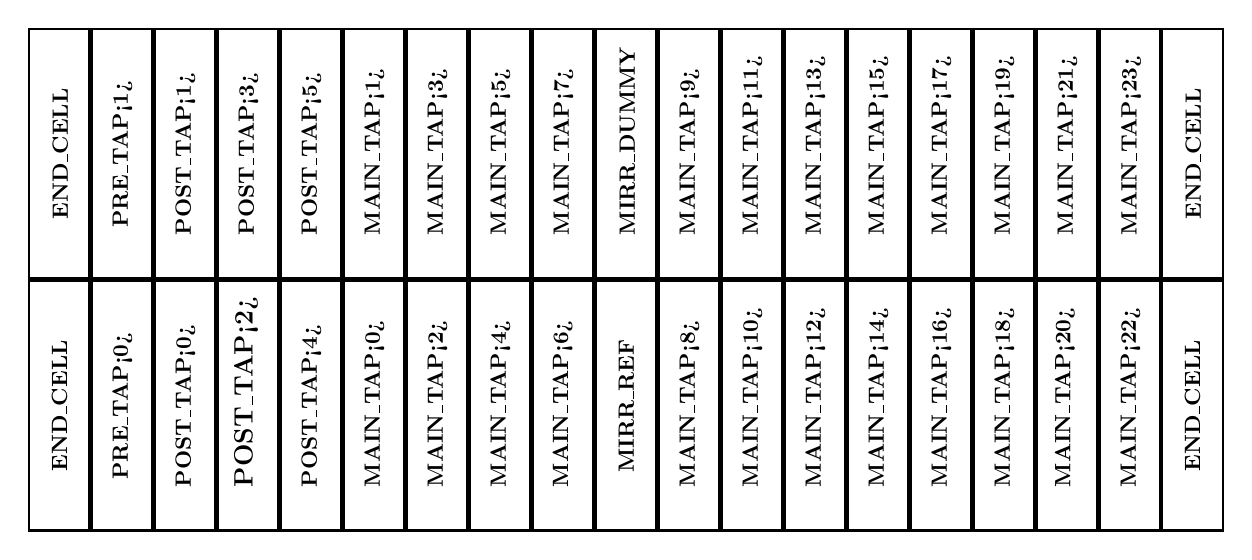
\begin{tikzpicture}[scale=0.8, transform shape]
		% Paths, nodes and wires:
		\node[shape=rectangle, draw, line width=1pt, minimum width=0.965cm, minimum height=3.965cm] at (1.5, 6){};
		\node[shape=rectangle, draw, line width=1pt, minimum width=0.965cm, minimum height=3.965cm] at (1.5, 2){};
		\node[shape=rectangle, rotate=90, minimum width=2.965cm, minimum height=0.715cm] at (1.5, 2){} node[anchor=center, align=center, text width=2.577cm, inner sep=6pt, rotate=90] at (1.5, 2){\textbf{PRE\_TAP<0>}};
		\node[shape=rectangle, rotate=90, minimum width=2.965cm, minimum height=0.715cm] at (1.5, 6){} node[anchor=center, align=center, text width=2.577cm, inner sep=6pt, rotate=90] at (1.5, 6){\textbf{PRE\_TAP<1>}};
		\node[shape=rectangle, draw, line width=1pt, minimum width=0.965cm, minimum height=3.965cm] at (2.5, 6){};
		\node[shape=rectangle, draw, line width=1pt, minimum width=0.965cm, minimum height=3.965cm] at (2.5, 2){};
		\node[shape=rectangle, rotate=90, minimum width=2.965cm, minimum height=0.715cm] at (2.5, 2){} node[anchor=center, align=center, text width=2.577cm, inner sep=6pt, rotate=90] at (2.5, 2){\textbf{POST\_TAP<0>}};
		\node[shape=rectangle, rotate=90, minimum width=2.965cm, minimum height=0.715cm] at (2.5, 6){} node[anchor=center, align=center, text width=2.577cm, inner sep=6pt, rotate=90] at (2.5, 6){\textbf{POST\_TAP<1>}};
		\node[shape=rectangle, draw, line width=1pt, minimum width=0.965cm, minimum height=3.965cm] at (3.5, 6){};
		\node[shape=rectangle, draw, line width=1pt, minimum width=0.965cm, minimum height=3.965cm] at (3.5, 2){};
		\node[shape=rectangle, rotate=90, minimum width=2.965cm, minimum height=0.715cm] at (3.462, 2){} node[anchor=center, align=center, text width=2.577cm, inner sep=6pt, rotate=90] at (3.462, 2){\large \textbf{POST\_TAP<2>}};
		\node[shape=rectangle, rotate=90, minimum width=2.965cm, minimum height=0.715cm] at (3.5, 6){} node[anchor=center, align=center, text width=2.577cm, inner sep=6pt, rotate=90] at (3.5, 6){\textbf{POST\_TAP<3>}};
		\node[shape=rectangle, draw, line width=1pt, minimum width=0.965cm, minimum height=3.965cm] at (4.5, 6){};
		\node[shape=rectangle, draw, line width=1pt, minimum width=0.965cm, minimum height=3.965cm] at (4.5, 2){};
		\node[shape=rectangle, rotate=90, minimum width=2.965cm, minimum height=0.715cm] at (4.5, 2){} node[anchor=center, align=center, text width=2.577cm, inner sep=6pt, rotate=90] at (4.5, 2){\textbf{POST\_TAP<4>}};
		\node[shape=rectangle, rotate=90, minimum width=2.965cm, minimum height=0.715cm] at (4.5, 6){} node[anchor=center, align=center, text width=2.577cm, inner sep=6pt, rotate=90] at (4.5, 6){\textbf{POST\_TAP<5>}};
		\node[shape=rectangle, draw, line width=1pt, minimum width=0.965cm, minimum height=3.965cm] at (5.5, 6){};
		\node[shape=rectangle, draw, line width=1pt, minimum width=0.965cm, minimum height=3.965cm] at (5.5, 2){};
		\node[shape=rectangle, rotate=90, minimum width=2.965cm, minimum height=0.715cm] at (5.5, 2){} node[anchor=center, align=center, text width=2.577cm, inner sep=6pt, rotate=90] at (5.5, 2){\textbf{MAIN\_TAP<0>}};
		\node[shape=rectangle, rotate=90, minimum width=2.965cm, minimum height=0.715cm] at (5.5, 6){} node[anchor=center, align=center, text width=2.577cm, inner sep=6pt, rotate=90] at (5.5, 6){\textbf{MAIN\_TAP<1>}};
		\node[shape=rectangle, draw, line width=1pt, minimum width=0.965cm, minimum height=3.965cm] at (6.5, 6){};
		\node[shape=rectangle, draw, line width=1pt, minimum width=0.965cm, minimum height=3.965cm] at (6.5, 2){};
		\node[shape=rectangle, rotate=90, minimum width=2.965cm, minimum height=0.715cm] at (6.5, 2){} node[anchor=center, align=center, text width=2.577cm, inner sep=6pt, rotate=90] at (6.5, 2){\textbf{MAIN\_TAP<2>}};
		\node[shape=rectangle, rotate=90, minimum width=2.965cm, minimum height=0.715cm] at (6.5, 6){} node[anchor=center, align=center, text width=2.577cm, inner sep=6pt, rotate=90] at (6.5, 6){\textbf{MAIN\_TAP<3>}};
		\node[shape=rectangle, draw, line width=1pt, minimum width=0.965cm, minimum height=3.965cm] at (7.5, 6){};
		\node[shape=rectangle, draw, line width=1pt, minimum width=0.965cm, minimum height=3.965cm] at (7.5, 2){};
		\node[shape=rectangle, rotate=90, minimum width=2.965cm, minimum height=0.715cm] at (7.5, 2){} node[anchor=center, align=center, text width=2.577cm, inner sep=6pt, rotate=90] at (7.5, 2){\textbf{MAIN\_TAP<4>}};
		\node[shape=rectangle, rotate=90, minimum width=2.965cm, minimum height=0.715cm] at (7.5, 6){} node[anchor=center, align=center, text width=2.577cm, inner sep=6pt, rotate=90] at (7.5, 6){\textbf{MAIN\_TAP<5>}};
		\node[shape=rectangle, draw, line width=1pt, minimum width=0.965cm, minimum height=3.965cm] at (8.5, 6){};
		\node[shape=rectangle, draw, line width=1pt, minimum width=0.965cm, minimum height=3.965cm] at (8.5, 2){};
		\node[shape=rectangle, rotate=90, minimum width=2.965cm, minimum height=0.715cm] at (8.487, 2){} node[anchor=center, align=center, text width=2.577cm, inner sep=6pt, rotate=90] at (8.487, 2){\textbf{MAIN\_TAP<6>}};
		\node[shape=rectangle, rotate=90, minimum width=2.965cm, minimum height=0.715cm] at (8.5, 6){} node[anchor=center, align=center, text width=2.577cm, inner sep=6pt, rotate=90] at (8.5, 6){\textbf{MAIN\_TAP<7>}};
		\node[shape=rectangle, draw, line width=1pt, minimum width=0.965cm, minimum height=3.965cm] at (10.5, 6){};
		\node[shape=rectangle, draw, line width=1pt, minimum width=0.965cm, minimum height=3.965cm] at (10.5, 2){};
		\node[shape=rectangle, rotate=90, minimum width=2.965cm, minimum height=0.715cm] at (10.5, 2){} node[anchor=center, align=center, text width=2.577cm, inner sep=6pt, rotate=90] at (10.5, 2){\textbf{MAIN\_TAP<8>}};
		\node[shape=rectangle, rotate=90, minimum width=2.965cm, minimum height=0.715cm] at (10.5, 6){} node[anchor=center, align=center, text width=2.577cm, inner sep=6pt, rotate=90] at (10.5, 6){\textbf{MAIN\_TAP<9>}};
		\node[shape=rectangle, draw, line width=1pt, minimum width=0.965cm, minimum height=3.965cm] at (11.5, 6){};
		\node[shape=rectangle, draw, line width=1pt, minimum width=0.965cm, minimum height=3.965cm] at (11.5, 2){};
		\node[shape=rectangle, rotate=90, minimum width=2.965cm, minimum height=0.715cm] at (11.5, 2){} node[anchor=center, align=center, text width=2.577cm, inner sep=6pt, rotate=90] at (11.5, 2){\textbf{MAIN\_TAP<10>}};
		\node[shape=rectangle, rotate=90, minimum width=2.965cm, minimum height=0.715cm] at (11.5, 6){} node[anchor=center, align=center, text width=2.577cm, inner sep=6pt, rotate=90] at (11.5, 6){\textbf{MAIN\_TAP<11>}};
		\node[shape=rectangle, draw, line width=1pt, minimum width=0.965cm, minimum height=3.965cm] at (12.5, 6){};
		\node[shape=rectangle, draw, line width=1pt, minimum width=0.965cm, minimum height=3.965cm] at (12.5, 2){};
		\node[shape=rectangle, rotate=90, minimum width=2.965cm, minimum height=0.715cm] at (12.5, 2){} node[anchor=center, align=center, text width=2.577cm, inner sep=6pt, rotate=90] at (12.5, 2){\textbf{MAIN\_TAP<12>}};
		\node[shape=rectangle, rotate=90, minimum width=2.965cm, minimum height=0.715cm] at (12.5, 6){} node[anchor=center, align=center, text width=2.577cm, inner sep=6pt, rotate=90] at (12.5, 6){\textbf{MAIN\_TAP<13>}};
		\node[shape=rectangle, draw, line width=1pt, minimum width=0.965cm, minimum height=3.965cm] at (13.5, 6){};
		\node[shape=rectangle, draw, line width=1pt, minimum width=0.965cm, minimum height=3.965cm] at (13.5, 2){};
		\node[shape=rectangle, rotate=90, minimum width=2.965cm, minimum height=0.715cm] at (13.5, 2){} node[anchor=center, align=center, text width=2.577cm, inner sep=6pt, rotate=90] at (13.5, 2){\textbf{MAIN\_TAP<14>}};
		\node[shape=rectangle, rotate=90, minimum width=2.965cm, minimum height=0.715cm] at (13.5, 6){} node[anchor=center, align=center, text width=2.577cm, inner sep=6pt, rotate=90] at (13.5, 6){\textbf{MAIN\_TAP<15>}};
		\node[shape=rectangle, draw, line width=1pt, minimum width=0.965cm, minimum height=3.965cm] at (14.5, 6){};
		\node[shape=rectangle, draw, line width=1pt, minimum width=0.965cm, minimum height=3.965cm] at (14.5, 2){};
		\node[shape=rectangle, rotate=90, minimum width=2.965cm, minimum height=0.715cm] at (14.5, 2){} node[anchor=center, align=center, text width=2.577cm, inner sep=6pt, rotate=90] at (14.5, 2){\textbf{MAIN\_TAP<16>}};
		\node[shape=rectangle, rotate=90, minimum width=2.965cm, minimum height=0.715cm] at (14.5, 6){} node[anchor=center, align=center, text width=2.577cm, inner sep=6pt, rotate=90] at (14.5, 6){\textbf{MAIN\_TAP<17>}};
		\node[shape=rectangle, draw, line width=1pt, minimum width=0.965cm, minimum height=3.965cm] at (15.5, 6){};
		\node[shape=rectangle, draw, line width=1pt, minimum width=0.965cm, minimum height=3.965cm] at (15.5, 2){};
		\node[shape=rectangle, rotate=90, minimum width=2.965cm, minimum height=0.715cm] at (15.5, 2){} node[anchor=center, align=center, text width=2.577cm, inner sep=6pt, rotate=90] at (15.5, 2){\textbf{MAIN\_TAP<18>}};
		\node[shape=rectangle, rotate=90, minimum width=2.965cm, minimum height=0.715cm] at (15.5, 6){} node[anchor=center, align=center, text width=2.577cm, inner sep=6pt, rotate=90] at (15.5, 6){\textbf{MAIN\_TAP<19>}};
		\node[shape=rectangle, draw, line width=1pt, minimum width=0.965cm, minimum height=3.965cm] at (16.5, 6){};
		\node[shape=rectangle, draw, line width=1pt, minimum width=0.965cm, minimum height=3.965cm] at (16.5, 2){};
		\node[shape=rectangle, rotate=90, minimum width=2.965cm, minimum height=0.715cm] at (16.462, 2){} node[anchor=center, align=center, text width=2.577cm, inner sep=6pt, rotate=90] at (16.462, 2){\textbf{MAIN\_TAP<20>}};
		\node[shape=rectangle, rotate=90, minimum width=2.965cm, minimum height=0.715cm] at (16.5, 6){} node[anchor=center, align=center, text width=2.577cm, inner sep=6pt, rotate=90] at (16.5, 6){\textbf{MAIN\_TAP<21>}};
		\node[shape=rectangle, draw, line width=1pt, minimum width=0.965cm, minimum height=3.965cm] at (17.5, 6){};
		\node[shape=rectangle, draw, line width=1pt, minimum width=0.965cm, minimum height=3.965cm] at (17.5, 2){};
		\node[shape=rectangle, rotate=90, minimum width=2.965cm, minimum height=0.715cm] at (17.5, 2){} node[anchor=center, align=center, text width=2.577cm, inner sep=6pt, rotate=90] at (17.5, 2){\textbf{MAIN\_TAP<22>}};
		\node[shape=rectangle, rotate=90, minimum width=2.965cm, minimum height=0.715cm] at (17.513, 6){} node[anchor=center, align=center, text width=2.577cm, inner sep=6pt, rotate=90] at (17.513, 6){\textbf{MAIN\_TAP<23>}};
		\node[shape=rectangle, draw, line width=1pt, minimum width=0.965cm, minimum height=3.965cm] at (18.487, 6){};
		\node[shape=rectangle, draw, line width=1pt, minimum width=0.965cm, minimum height=3.965cm] at (18.487, 2){};
		\node[shape=rectangle, rotate=90, minimum width=2.965cm, minimum height=0.715cm] at (18.487, 2){} node[anchor=center, align=center, text width=2.577cm, inner sep=6pt, rotate=90] at (18.487, 2){\textbf{END\_CELL}};
		\node[shape=rectangle, rotate=90, minimum width=2.965cm, minimum height=0.715cm] at (18.5, 6){} node[anchor=center, align=center, text width=2.577cm, inner sep=6pt, rotate=90] at (18.5, 6){\textbf{END\_CELL}};
		\node[shape=rectangle, draw, line width=1pt, minimum width=0.965cm, minimum height=3.965cm] at (0.5, 6){};
		\node[shape=rectangle, draw, line width=1pt, minimum width=0.965cm, minimum height=3.965cm] at (0.5, 2){};
		\node[shape=rectangle, rotate=90, minimum width=2.965cm, minimum height=0.715cm] at (0.5, 2){} node[anchor=center, align=center, text width=2.577cm, inner sep=6pt, rotate=90] at (0.5, 2){\textbf{END\_CELL}};
		\node[shape=rectangle, rotate=90, minimum width=2.965cm, minimum height=0.715cm] at (0.513, 6){} node[anchor=center, align=center, text width=2.577cm, inner sep=6pt, rotate=90] at (0.513, 6){\textbf{END\_CELL}};
		\node[shape=rectangle, draw, line width=1pt, minimum width=0.965cm, minimum height=3.965cm] at (9.5, 6){};
		\node[shape=rectangle, draw, line width=1pt, minimum width=0.965cm, minimum height=3.965cm] at (9.5, 2){};
		\node[shape=rectangle, rotate=90, minimum width=2.965cm, minimum height=0.715cm] at (9.5, 2){} node[anchor=center, align=center, text width=2.577cm, inner sep=6pt, rotate=90] at (9.5, 2){\textbf{MIRR\_REF}};
		\node[shape=rectangle, rotate=90, minimum width=2.965cm, minimum height=0.715cm] at (9.513, 6){} node[anchor=center, align=center, text width=2.577cm, inner sep=6pt, rotate=90] at (9.513, 6){\textbf{MIRR\_DUMMY}};
	\end{tikzpicture}
\caption{Driver layout floorplan}
\label{fig:driver_layout_floorplan}
\end{figure}

Establishing this boundary early in the design process had two important consequences for the remainder of the layout work:

\begin{enumerate}
	\item It allowed considerably more freedom in how the internal layout of each standard cell was arranged, since the usable area of the cell was clearly and unambiguously defined from the outset; routing and device placement within the cell could be optimized freely, provided the result remained consistent with the fixed boundary and edge connections.
	\item Defining the boundary in this way meant that the connection points between adjacent cells had to be given careful consideration from the earliest stages of the layout design, rather than being treated as an afterthought once individual cells were already complete. Since these edge connections directly determine whether cells can be abutted correctly, ensuring their placement and geometry were consistent across all tap unit instances was essential to the success of the modular approach.
\end{enumerate}

\begin{figure}[h]
	\begin{subfigure}[b]{0.49\textwidth}
		\resizebox{1.1\linewidth}{!}{
		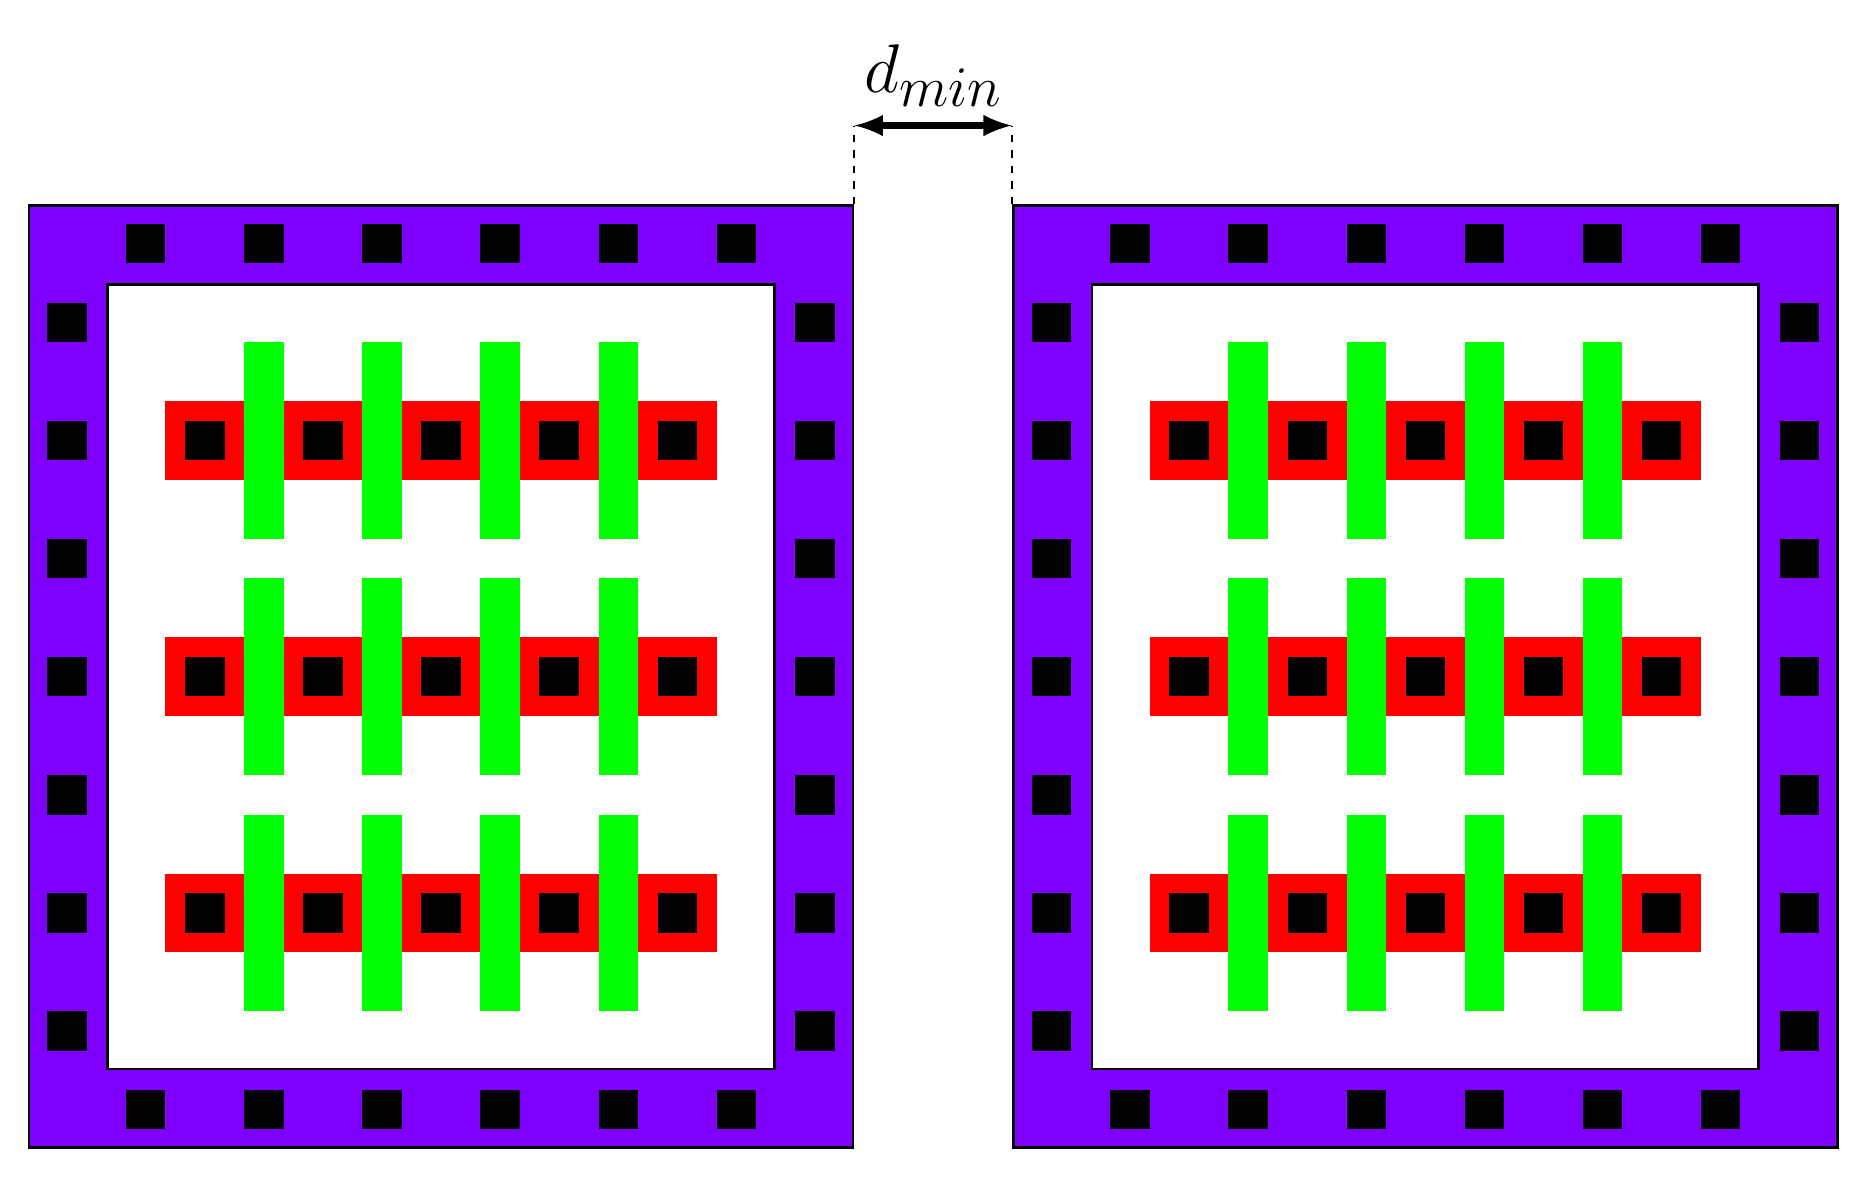
\begin{tikzpicture}[transform shape]
			% Paths, nodes and wires:
			\node[shape=rectangle, fill={rgb,255:red,128;green,0;blue,255}, draw, line width=1pt, minimum width=10.465cm, minimum height=11.965cm] at (5.25, 6){};
			\node[shape=rectangle, fill={rgb,255:red,255;green,255;blue,255}, draw, line width=1pt, minimum width=8.465cm, minimum height=9.965cm] at (5.25, 6){};
			\node[shape=rectangle, fill={rgb,255:red,0;green,0;blue,0}, draw, line width=1pt, minimum width=0.465cm, minimum height=0.465cm] at (0.5, 7.5){};
			\node[shape=rectangle, fill={rgb,255:red,0;green,0;blue,0}, draw, line width=1pt, minimum width=0.465cm, minimum height=0.465cm] at (0.5, 10.5){};
			\node[shape=rectangle, fill={rgb,255:red,0;green,0;blue,0}, draw, line width=1pt, minimum width=0.465cm, minimum height=0.465cm] at (0.5, 9){};
			\node[shape=rectangle, fill={rgb,255:red,0;green,0;blue,0}, draw, line width=1pt, minimum width=0.465cm, minimum height=0.465cm] at (0.5, 6){};
			\node[shape=rectangle, fill={rgb,255:red,0;green,0;blue,0}, draw, line width=1pt, minimum width=0.465cm, minimum height=0.465cm] at (0.5, 4.5){};
			\node[shape=rectangle, fill={rgb,255:red,0;green,0;blue,0}, draw, line width=1pt, minimum width=0.465cm, minimum height=0.465cm] at (0.5, 3){};
			\node[shape=rectangle, fill={rgb,255:red,255;green,0;blue,0}, draw={rgb,255:red,255;green,0;blue,0}, line width=1pt, minimum width=6.965cm, minimum height=0.965cm] at (5.25, 9){};
			\node[shape=rectangle, fill={rgb,255:red,0;green,0;blue,0}, draw, line width=1pt, minimum width=0.465cm, minimum height=0.465cm] at (2.25, 9){};
			\node[shape=rectangle, fill={rgb,255:red,0;green,255;blue,0}, draw={rgb,255:red,0;green,255;blue,0}, line width=1pt, minimum width=0.465cm, minimum height=2.465cm] at (3, 9){};
			\node[shape=rectangle, fill={rgb,255:red,0;green,0;blue,0}, draw, line width=1pt, minimum width=0.465cm, minimum height=0.465cm] at (3.75, 9){};
			\node[shape=rectangle, fill={rgb,255:red,0;green,255;blue,0}, draw={rgb,255:red,0;green,255;blue,0}, line width=1pt, minimum width=0.465cm, minimum height=2.465cm] at (4.5, 9){};
			\node[shape=rectangle, fill={rgb,255:red,0;green,0;blue,0}, draw, line width=1pt, minimum width=0.465cm, minimum height=0.465cm] at (5.25, 9){};
			\node[shape=rectangle, fill={rgb,255:red,0;green,255;blue,0}, draw={rgb,255:red,0;green,255;blue,0}, line width=1pt, minimum width=0.465cm, minimum height=2.465cm] at (6, 9){};
			\node[shape=rectangle, fill={rgb,255:red,0;green,0;blue,0}, draw, line width=1pt, minimum width=0.465cm, minimum height=0.465cm] at (6.75, 9){};
			\node[shape=rectangle, fill={rgb,255:red,0;green,255;blue,0}, draw={rgb,255:red,0;green,255;blue,0}, line width=1pt, minimum width=0.465cm, minimum height=2.465cm] at (7.5, 9){};
			\node[shape=rectangle, fill={rgb,255:red,0;green,0;blue,0}, draw, line width=1pt, minimum width=0.465cm, minimum height=0.465cm] at (8.25, 9){};
			\node[shape=rectangle, fill={rgb,255:red,255;green,0;blue,0}, draw={rgb,255:red,255;green,0;blue,0}, line width=1pt, minimum width=6.965cm, minimum height=0.965cm] at (5.25, 6){};
			\node[shape=rectangle, fill={rgb,255:red,0;green,0;blue,0}, draw, line width=1pt, minimum width=0.465cm, minimum height=0.465cm] at (2.25, 6){};
			\node[shape=rectangle, fill={rgb,255:red,0;green,255;blue,0}, draw={rgb,255:red,0;green,255;blue,0}, line width=1pt, minimum width=0.465cm, minimum height=2.465cm] at (3, 6){};
			\node[shape=rectangle, fill={rgb,255:red,0;green,0;blue,0}, draw, line width=1pt, minimum width=0.465cm, minimum height=0.465cm] at (3.75, 6){};
			\node[shape=rectangle, fill={rgb,255:red,0;green,255;blue,0}, draw={rgb,255:red,0;green,255;blue,0}, line width=1pt, minimum width=0.465cm, minimum height=2.465cm] at (4.5, 6){};
			\node[shape=rectangle, fill={rgb,255:red,0;green,0;blue,0}, draw, line width=1pt, minimum width=0.465cm, minimum height=0.465cm] at (5.25, 6){};
			\node[shape=rectangle, fill={rgb,255:red,0;green,255;blue,0}, draw={rgb,255:red,0;green,255;blue,0}, line width=1pt, minimum width=0.465cm, minimum height=2.465cm] at (6, 6){};
			\node[shape=rectangle, fill={rgb,255:red,0;green,0;blue,0}, draw, line width=1pt, minimum width=0.465cm, minimum height=0.465cm] at (6.75, 6){};
			\node[shape=rectangle, fill={rgb,255:red,0;green,255;blue,0}, draw={rgb,255:red,0;green,255;blue,0}, line width=1pt, minimum width=0.465cm, minimum height=2.465cm] at (7.5, 6){};
			\node[shape=rectangle, fill={rgb,255:red,0;green,0;blue,0}, draw, line width=1pt, minimum width=0.465cm, minimum height=0.465cm] at (8.25, 6){};
			\node[shape=rectangle, fill={rgb,255:red,255;green,0;blue,0}, draw={rgb,255:red,255;green,0;blue,0}, line width=1pt, minimum width=6.965cm, minimum height=0.965cm] at (5.25, 3){};
			\node[shape=rectangle, fill={rgb,255:red,0;green,0;blue,0}, draw, line width=1pt, minimum width=0.465cm, minimum height=0.465cm] at (2.25, 3){};
			\node[shape=rectangle, fill={rgb,255:red,0;green,255;blue,0}, draw={rgb,255:red,0;green,255;blue,0}, line width=1pt, minimum width=0.465cm, minimum height=2.465cm] at (3, 3){};
			\node[shape=rectangle, fill={rgb,255:red,0;green,0;blue,0}, draw, line width=1pt, minimum width=0.465cm, minimum height=0.465cm] at (3.75, 3){};
			\node[shape=rectangle, fill={rgb,255:red,0;green,255;blue,0}, draw={rgb,255:red,0;green,255;blue,0}, line width=1pt, minimum width=0.465cm, minimum height=2.465cm] at (4.5, 3){};
			\node[shape=rectangle, fill={rgb,255:red,0;green,0;blue,0}, draw, line width=1pt, minimum width=0.465cm, minimum height=0.465cm] at (5.25, 3){};
			\node[shape=rectangle, fill={rgb,255:red,0;green,255;blue,0}, draw={rgb,255:red,0;green,255;blue,0}, line width=1pt, minimum width=0.465cm, minimum height=2.465cm] at (6, 3){};
			\node[shape=rectangle, fill={rgb,255:red,0;green,0;blue,0}, draw, line width=1pt, minimum width=0.465cm, minimum height=0.465cm] at (6.75, 3){};
			\node[shape=rectangle, fill={rgb,255:red,0;green,255;blue,0}, draw={rgb,255:red,0;green,255;blue,0}, line width=1pt, minimum width=0.465cm, minimum height=2.465cm] at (7.5, 3){};
			\node[shape=rectangle, fill={rgb,255:red,0;green,0;blue,0}, draw, line width=1pt, minimum width=0.465cm, minimum height=0.465cm] at (8.25, 3){};
			\node[shape=rectangle, fill={rgb,255:red,0;green,0;blue,0}, draw, line width=1pt, minimum width=0.465cm, minimum height=0.465cm] at (10, 7.5){};
			\node[shape=rectangle, fill={rgb,255:red,0;green,0;blue,0}, draw, line width=1pt, minimum width=0.465cm, minimum height=0.465cm] at (10, 10.5){};
			\node[shape=rectangle, fill={rgb,255:red,0;green,0;blue,0}, draw, line width=1pt, minimum width=0.465cm, minimum height=0.465cm] at (10, 9){};
			\node[shape=rectangle, fill={rgb,255:red,0;green,0;blue,0}, draw, line width=1pt, minimum width=0.465cm, minimum height=0.465cm] at (10, 6){};
			\node[shape=rectangle, fill={rgb,255:red,0;green,0;blue,0}, draw, line width=1pt, minimum width=0.465cm, minimum height=0.465cm] at (10, 4.5){};
			\node[shape=rectangle, fill={rgb,255:red,0;green,0;blue,0}, draw, line width=1pt, minimum width=0.465cm, minimum height=0.465cm] at (10, 3){};
			\node[shape=rectangle, fill={rgb,255:red,0;green,0;blue,0}, draw, line width=1pt, minimum width=0.465cm, minimum height=0.465cm] at (0.5, 1.5){};
			\node[shape=rectangle, fill={rgb,255:red,0;green,0;blue,0}, draw, line width=1pt, minimum width=0.465cm, minimum height=0.465cm] at (10, 1.5){};
			\node[shape=rectangle, fill={rgb,255:red,0;green,0;blue,0}, draw, line width=1pt, minimum width=0.465cm, minimum height=0.465cm] at (1.5, 11.5){};
			\node[shape=rectangle, fill={rgb,255:red,0;green,0;blue,0}, draw, line width=1pt, minimum width=0.465cm, minimum height=0.465cm] at (3, 11.5){};
			\node[shape=rectangle, fill={rgb,255:red,0;green,0;blue,0}, draw, line width=1pt, minimum width=0.465cm, minimum height=0.465cm] at (4.5, 11.5){};
			\node[shape=rectangle, fill={rgb,255:red,0;green,0;blue,0}, draw, line width=1pt, minimum width=0.465cm, minimum height=0.465cm] at (6, 11.5){};
			\node[shape=rectangle, fill={rgb,255:red,0;green,0;blue,0}, draw, line width=1pt, minimum width=0.465cm, minimum height=0.465cm] at (7.5, 11.5){};
			\node[shape=rectangle, fill={rgb,255:red,0;green,0;blue,0}, draw, line width=1pt, minimum width=0.465cm, minimum height=0.465cm] at (9, 11.5){};
			\node[shape=rectangle, fill={rgb,255:red,0;green,0;blue,0}, draw, line width=1pt, minimum width=0.465cm, minimum height=0.465cm] at (1.5, 0.5){};
			\node[shape=rectangle, fill={rgb,255:red,0;green,0;blue,0}, draw, line width=1pt, minimum width=0.465cm, minimum height=0.465cm] at (3, 0.5){};
			\node[shape=rectangle, fill={rgb,255:red,0;green,0;blue,0}, draw, line width=1pt, minimum width=0.465cm, minimum height=0.465cm] at (4.5, 0.5){};
			\node[shape=rectangle, fill={rgb,255:red,0;green,0;blue,0}, draw, line width=1pt, minimum width=0.465cm, minimum height=0.465cm] at (6, 0.5){};
			\node[shape=rectangle, fill={rgb,255:red,0;green,0;blue,0}, draw, line width=1pt, minimum width=0.465cm, minimum height=0.465cm] at (7.5, 0.5){};
			\node[shape=rectangle, fill={rgb,255:red,0;green,0;blue,0}, draw, line width=1pt, minimum width=0.465cm, minimum height=0.465cm] at (9, 0.5){};
			\node[shape=rectangle, fill={rgb,255:red,128;green,0;blue,255}, draw, line width=1pt, minimum width=10.465cm, minimum height=11.965cm] at (17.75, 6){};
			\node[shape=rectangle, fill={rgb,255:red,255;green,255;blue,255}, draw, line width=1pt, minimum width=8.465cm, minimum height=9.965cm] at (17.75, 6){};
			\node[shape=rectangle, fill={rgb,255:red,0;green,0;blue,0}, draw, line width=1pt, minimum width=0.465cm, minimum height=0.465cm] at (13, 7.5){};
			\node[shape=rectangle, fill={rgb,255:red,0;green,0;blue,0}, draw, line width=1pt, minimum width=0.465cm, minimum height=0.465cm] at (13, 10.5){};
			\node[shape=rectangle, fill={rgb,255:red,0;green,0;blue,0}, draw, line width=1pt, minimum width=0.465cm, minimum height=0.465cm] at (13, 9){};
			\node[shape=rectangle, fill={rgb,255:red,0;green,0;blue,0}, draw, line width=1pt, minimum width=0.465cm, minimum height=0.465cm] at (13, 6){};
			\node[shape=rectangle, fill={rgb,255:red,0;green,0;blue,0}, draw, line width=1pt, minimum width=0.465cm, minimum height=0.465cm] at (13, 4.5){};
			\node[shape=rectangle, fill={rgb,255:red,0;green,0;blue,0}, draw, line width=1pt, minimum width=0.465cm, minimum height=0.465cm] at (13, 3){};
			\node[shape=rectangle, fill={rgb,255:red,255;green,0;blue,0}, draw={rgb,255:red,255;green,0;blue,0}, line width=1pt, minimum width=6.965cm, minimum height=0.965cm] at (17.75, 9){};
			\node[shape=rectangle, fill={rgb,255:red,0;green,0;blue,0}, draw, line width=1pt, minimum width=0.465cm, minimum height=0.465cm] at (14.75, 9){};
			\node[shape=rectangle, fill={rgb,255:red,0;green,255;blue,0}, draw={rgb,255:red,0;green,255;blue,0}, line width=1pt, minimum width=0.465cm, minimum height=2.465cm] at (15.5, 9){};
			\node[shape=rectangle, fill={rgb,255:red,0;green,0;blue,0}, draw, line width=1pt, minimum width=0.465cm, minimum height=0.465cm] at (16.25, 9){};
			\node[shape=rectangle, fill={rgb,255:red,0;green,255;blue,0}, draw={rgb,255:red,0;green,255;blue,0}, line width=1pt, minimum width=0.465cm, minimum height=2.465cm] at (17, 9){};
			\node[shape=rectangle, fill={rgb,255:red,0;green,0;blue,0}, draw, line width=1pt, minimum width=0.465cm, minimum height=0.465cm] at (17.75, 9){};
			\node[shape=rectangle, fill={rgb,255:red,0;green,255;blue,0}, draw={rgb,255:red,0;green,255;blue,0}, line width=1pt, minimum width=0.465cm, minimum height=2.465cm] at (18.5, 9){};
			\node[shape=rectangle, fill={rgb,255:red,0;green,0;blue,0}, draw, line width=1pt, minimum width=0.465cm, minimum height=0.465cm] at (19.25, 9){};
			\node[shape=rectangle, fill={rgb,255:red,0;green,255;blue,0}, draw={rgb,255:red,0;green,255;blue,0}, line width=1pt, minimum width=0.465cm, minimum height=2.465cm] at (20, 9){};
			\node[shape=rectangle, fill={rgb,255:red,0;green,0;blue,0}, draw, line width=1pt, minimum width=0.465cm, minimum height=0.465cm] at (20.75, 9){};
			\node[shape=rectangle, fill={rgb,255:red,255;green,0;blue,0}, draw={rgb,255:red,255;green,0;blue,0}, line width=1pt, minimum width=6.965cm, minimum height=0.965cm] at (17.75, 6){};
			\node[shape=rectangle, fill={rgb,255:red,0;green,0;blue,0}, draw, line width=1pt, minimum width=0.465cm, minimum height=0.465cm] at (14.75, 6){};
			\node[shape=rectangle, fill={rgb,255:red,0;green,255;blue,0}, draw={rgb,255:red,0;green,255;blue,0}, line width=1pt, minimum width=0.465cm, minimum height=2.465cm] at (15.5, 6){};
			\node[shape=rectangle, fill={rgb,255:red,0;green,0;blue,0}, draw, line width=1pt, minimum width=0.465cm, minimum height=0.465cm] at (16.25, 6){};
			\node[shape=rectangle, fill={rgb,255:red,0;green,255;blue,0}, draw={rgb,255:red,0;green,255;blue,0}, line width=1pt, minimum width=0.465cm, minimum height=2.465cm] at (17, 6){};
			\node[shape=rectangle, fill={rgb,255:red,0;green,0;blue,0}, draw, line width=1pt, minimum width=0.465cm, minimum height=0.465cm] at (17.75, 6){};
			\node[shape=rectangle, fill={rgb,255:red,0;green,255;blue,0}, draw={rgb,255:red,0;green,255;blue,0}, line width=1pt, minimum width=0.465cm, minimum height=2.465cm] at (18.5, 6){};
			\node[shape=rectangle, fill={rgb,255:red,0;green,0;blue,0}, draw, line width=1pt, minimum width=0.465cm, minimum height=0.465cm] at (19.25, 6){};
			\node[shape=rectangle, fill={rgb,255:red,0;green,255;blue,0}, draw={rgb,255:red,0;green,255;blue,0}, line width=1pt, minimum width=0.465cm, minimum height=2.465cm] at (20, 6){};
			\node[shape=rectangle, fill={rgb,255:red,0;green,0;blue,0}, draw, line width=1pt, minimum width=0.465cm, minimum height=0.465cm] at (20.75, 6){};
			\node[shape=rectangle, fill={rgb,255:red,255;green,0;blue,0}, draw={rgb,255:red,255;green,0;blue,0}, line width=1pt, minimum width=6.965cm, minimum height=0.965cm] at (17.75, 3){};
			\node[shape=rectangle, fill={rgb,255:red,0;green,0;blue,0}, draw, line width=1pt, minimum width=0.465cm, minimum height=0.465cm] at (14.75, 3){};
			\node[shape=rectangle, fill={rgb,255:red,0;green,255;blue,0}, draw={rgb,255:red,0;green,255;blue,0}, line width=1pt, minimum width=0.465cm, minimum height=2.465cm] at (15.5, 3){};
			\node[shape=rectangle, fill={rgb,255:red,0;green,0;blue,0}, draw, line width=1pt, minimum width=0.465cm, minimum height=0.465cm] at (16.25, 3){};
			\node[shape=rectangle, fill={rgb,255:red,0;green,255;blue,0}, draw={rgb,255:red,0;green,255;blue,0}, line width=1pt, minimum width=0.465cm, minimum height=2.465cm] at (17, 3){};
			\node[shape=rectangle, fill={rgb,255:red,0;green,0;blue,0}, draw, line width=1pt, minimum width=0.465cm, minimum height=0.465cm] at (17.75, 3){};
			\node[shape=rectangle, fill={rgb,255:red,0;green,255;blue,0}, draw={rgb,255:red,0;green,255;blue,0}, line width=1pt, minimum width=0.465cm, minimum height=2.465cm] at (18.5, 3){};
			\node[shape=rectangle, fill={rgb,255:red,0;green,0;blue,0}, draw, line width=1pt, minimum width=0.465cm, minimum height=0.465cm] at (19.25, 3){};
			\node[shape=rectangle, fill={rgb,255:red,0;green,255;blue,0}, draw={rgb,255:red,0;green,255;blue,0}, line width=1pt, minimum width=0.465cm, minimum height=2.465cm] at (20, 3){};
			\node[shape=rectangle, fill={rgb,255:red,0;green,0;blue,0}, draw, line width=1pt, minimum width=0.465cm, minimum height=0.465cm] at (20.75, 3){};
			\node[shape=rectangle, fill={rgb,255:red,0;green,0;blue,0}, draw, line width=1pt, minimum width=0.465cm, minimum height=0.465cm] at (22.5, 7.5){};
			\node[shape=rectangle, fill={rgb,255:red,0;green,0;blue,0}, draw, line width=1pt, minimum width=0.465cm, minimum height=0.465cm] at (22.5, 10.5){};
			\node[shape=rectangle, fill={rgb,255:red,0;green,0;blue,0}, draw, line width=1pt, minimum width=0.465cm, minimum height=0.465cm] at (22.5, 9){};
			\node[shape=rectangle, fill={rgb,255:red,0;green,0;blue,0}, draw, line width=1pt, minimum width=0.465cm, minimum height=0.465cm] at (22.5, 6){};
			\node[shape=rectangle, fill={rgb,255:red,0;green,0;blue,0}, draw, line width=1pt, minimum width=0.465cm, minimum height=0.465cm] at (22.5, 4.5){};
			\node[shape=rectangle, fill={rgb,255:red,0;green,0;blue,0}, draw, line width=1pt, minimum width=0.465cm, minimum height=0.465cm] at (22.5, 3){};
			\node[shape=rectangle, fill={rgb,255:red,0;green,0;blue,0}, draw, line width=1pt, minimum width=0.465cm, minimum height=0.465cm] at (13, 1.5){};
			\node[shape=rectangle, fill={rgb,255:red,0;green,0;blue,0}, draw, line width=1pt, minimum width=0.465cm, minimum height=0.465cm] at (22.5, 1.5){};
			\node[shape=rectangle, fill={rgb,255:red,0;green,0;blue,0}, draw, line width=1pt, minimum width=0.465cm, minimum height=0.465cm] at (14, 11.5){};
			\node[shape=rectangle, fill={rgb,255:red,0;green,0;blue,0}, draw, line width=1pt, minimum width=0.465cm, minimum height=0.465cm] at (15.5, 11.5){};
			\node[shape=rectangle, fill={rgb,255:red,0;green,0;blue,0}, draw, line width=1pt, minimum width=0.465cm, minimum height=0.465cm] at (17, 11.5){};
			\node[shape=rectangle, fill={rgb,255:red,0;green,0;blue,0}, draw, line width=1pt, minimum width=0.465cm, minimum height=0.465cm] at (18.5, 11.5){};
			\node[shape=rectangle, fill={rgb,255:red,0;green,0;blue,0}, draw, line width=1pt, minimum width=0.465cm, minimum height=0.465cm] at (20, 11.5){};
			\node[shape=rectangle, fill={rgb,255:red,0;green,0;blue,0}, draw, line width=1pt, minimum width=0.465cm, minimum height=0.465cm] at (21.5, 11.5){};
			\node[shape=rectangle, fill={rgb,255:red,0;green,0;blue,0}, draw, line width=1pt, minimum width=0.465cm, minimum height=0.465cm] at (14, 0.5){};
			\node[shape=rectangle, fill={rgb,255:red,0;green,0;blue,0}, draw, line width=1pt, minimum width=0.465cm, minimum height=0.465cm] at (15.5, 0.5){};
			\node[shape=rectangle, fill={rgb,255:red,0;green,0;blue,0}, draw, line width=1pt, minimum width=0.465cm, minimum height=0.465cm] at (17, 0.5){};
			\node[shape=rectangle, fill={rgb,255:red,0;green,0;blue,0}, draw, line width=1pt, minimum width=0.465cm, minimum height=0.465cm] at (18.5, 0.5){};
			\node[shape=rectangle, fill={rgb,255:red,0;green,0;blue,0}, draw, line width=1pt, minimum width=0.465cm, minimum height=0.465cm] at (20, 0.5){};
			\node[shape=rectangle, fill={rgb,255:red,0;green,0;blue,0}, draw, line width=1pt, minimum width=0.465cm, minimum height=0.465cm] at (21.5, 0.5){};
			\draw[line width=2.5pt, latex-latex] (12.5, 13) -- (10.5, 13);
			\draw[line width=0.7pt, dash pattern={on 2.8pt off 2.8pt}] (10.5, 12) -- (10.5, 13);
			\draw[line width=0.7pt, dash pattern={on 2.8pt off 2.8pt}] (12.5, 12) -- (12.5, 13);
			\node[shape=rectangle, minimum width=2.465cm, minimum height=1.715cm] at (11.5, 13.375){} node[anchor=north, align=center, text width=2.077cm, inner sep=6pt] at (11.5, 14.25){\Huge $d_{min}$};
		\end{tikzpicture}
		}
		\caption{Non-abutted layout with separate guard rings}\label{fig:non_abutted}
	\end{subfigure}
	\begin{subfigure}[b]{0.49\textwidth}
		\centering
		\resizebox{0.8\textwidth}{!}{
		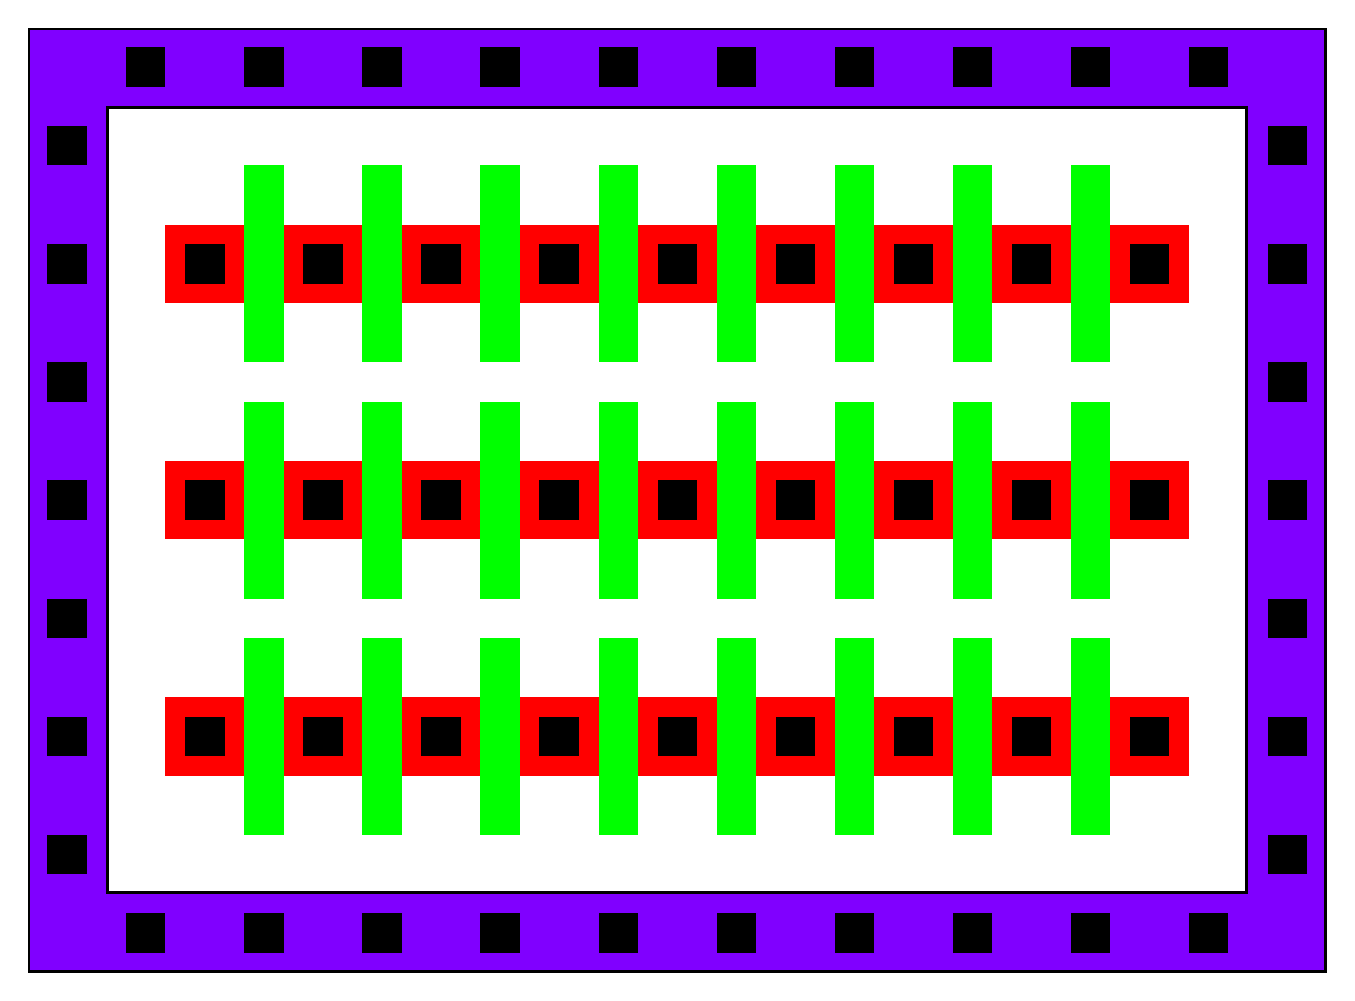
\begin{tikzpicture}[transform shape]
			% Paths, nodes and wires:
			\node[shape=rectangle, fill={rgb,255:red,128;green,0;blue,255}, draw, line width=1pt, minimum width=16.465cm, minimum height=11.965cm] at (8.25, 6){};
			\node[shape=rectangle, fill={rgb,255:red,255;green,255;blue,255}, draw, line width=1pt, minimum width=14.465cm, minimum height=9.965cm] at (8.25, 6){};
			\node[shape=rectangle, fill={rgb,255:red,0;green,0;blue,0}, draw, line width=1pt, minimum width=0.465cm, minimum height=0.465cm] at (0.5, 7.5){};
			\node[shape=rectangle, fill={rgb,255:red,0;green,0;blue,0}, draw, line width=1pt, minimum width=0.465cm, minimum height=0.465cm] at (0.5, 10.5){};
			\node[shape=rectangle, fill={rgb,255:red,0;green,0;blue,0}, draw, line width=1pt, minimum width=0.465cm, minimum height=0.465cm] at (0.5, 9){};
			\node[shape=rectangle, fill={rgb,255:red,0;green,0;blue,0}, draw, line width=1pt, minimum width=0.465cm, minimum height=0.465cm] at (0.5, 6){};
			\node[shape=rectangle, fill={rgb,255:red,0;green,0;blue,0}, draw, line width=1pt, minimum width=0.465cm, minimum height=0.465cm] at (0.5, 4.5){};
			\node[shape=rectangle, fill={rgb,255:red,0;green,0;blue,0}, draw, line width=1pt, minimum width=0.465cm, minimum height=0.465cm] at (0.5, 3){};
			\node[shape=rectangle, fill={rgb,255:red,255;green,0;blue,0}, draw={rgb,255:red,255;green,0;blue,0}, line width=1pt, minimum width=12.965cm, minimum height=0.965cm] at (8.25, 9){};
			\node[shape=rectangle, fill={rgb,255:red,0;green,0;blue,0}, draw, line width=1pt, minimum width=0.465cm, minimum height=0.465cm] at (2.25, 9){};
			\node[shape=rectangle, fill={rgb,255:red,0;green,255;blue,0}, draw={rgb,255:red,0;green,255;blue,0}, line width=1pt, minimum width=0.465cm, minimum height=2.465cm] at (3, 9){};
			\node[shape=rectangle, fill={rgb,255:red,0;green,0;blue,0}, draw, line width=1pt, minimum width=0.465cm, minimum height=0.465cm] at (3.75, 9){};
			\node[shape=rectangle, fill={rgb,255:red,0;green,255;blue,0}, draw={rgb,255:red,0;green,255;blue,0}, line width=1pt, minimum width=0.465cm, minimum height=2.465cm] at (4.5, 9){};
			\node[shape=rectangle, fill={rgb,255:red,0;green,0;blue,0}, draw, line width=1pt, minimum width=0.465cm, minimum height=0.465cm] at (5.25, 9){};
			\node[shape=rectangle, fill={rgb,255:red,0;green,255;blue,0}, draw={rgb,255:red,0;green,255;blue,0}, line width=1pt, minimum width=0.465cm, minimum height=2.465cm] at (6, 9){};
			\node[shape=rectangle, fill={rgb,255:red,0;green,0;blue,0}, draw, line width=1pt, minimum width=0.465cm, minimum height=0.465cm] at (6.75, 9){};
			\node[shape=rectangle, fill={rgb,255:red,0;green,255;blue,0}, draw={rgb,255:red,0;green,255;blue,0}, line width=1pt, minimum width=0.465cm, minimum height=2.465cm] at (7.5, 9){};
			\node[shape=rectangle, fill={rgb,255:red,255;green,0;blue,0}, draw={rgb,255:red,255;green,0;blue,0}, line width=1pt, minimum width=12.965cm, minimum height=0.965cm] at (8.25, 6){};
			\node[shape=rectangle, fill={rgb,255:red,0;green,0;blue,0}, draw, line width=1pt, minimum width=0.465cm, minimum height=0.465cm] at (2.25, 6){};
			\node[shape=rectangle, fill={rgb,255:red,0;green,255;blue,0}, draw={rgb,255:red,0;green,255;blue,0}, line width=1pt, minimum width=0.465cm, minimum height=2.465cm] at (3, 6){};
			\node[shape=rectangle, fill={rgb,255:red,0;green,0;blue,0}, draw, line width=1pt, minimum width=0.465cm, minimum height=0.465cm] at (3.75, 6){};
			\node[shape=rectangle, fill={rgb,255:red,0;green,255;blue,0}, draw={rgb,255:red,0;green,255;blue,0}, line width=1pt, minimum width=0.465cm, minimum height=2.465cm] at (4.5, 6){};
			\node[shape=rectangle, fill={rgb,255:red,0;green,0;blue,0}, draw, line width=1pt, minimum width=0.465cm, minimum height=0.465cm] at (5.25, 6){};
			\node[shape=rectangle, fill={rgb,255:red,0;green,255;blue,0}, draw={rgb,255:red,0;green,255;blue,0}, line width=1pt, minimum width=0.465cm, minimum height=2.465cm] at (6, 6){};
			\node[shape=rectangle, fill={rgb,255:red,0;green,0;blue,0}, draw, line width=1pt, minimum width=0.465cm, minimum height=0.465cm] at (6.75, 6){};
			\node[shape=rectangle, fill={rgb,255:red,0;green,255;blue,0}, draw={rgb,255:red,0;green,255;blue,0}, line width=1pt, minimum width=0.465cm, minimum height=2.465cm] at (7.5, 6){};
			\node[shape=rectangle, fill={rgb,255:red,255;green,0;blue,0}, draw={rgb,255:red,255;green,0;blue,0}, line width=1pt, minimum width=12.965cm, minimum height=0.965cm] at (8.25, 3){};
			\node[shape=rectangle, fill={rgb,255:red,0;green,0;blue,0}, draw, line width=1pt, minimum width=0.465cm, minimum height=0.465cm] at (2.25, 3){};
			\node[shape=rectangle, fill={rgb,255:red,0;green,255;blue,0}, draw={rgb,255:red,0;green,255;blue,0}, line width=1pt, minimum width=0.465cm, minimum height=2.465cm] at (3, 3){};
			\node[shape=rectangle, fill={rgb,255:red,0;green,0;blue,0}, draw, line width=1pt, minimum width=0.465cm, minimum height=0.465cm] at (3.75, 3){};
			\node[shape=rectangle, fill={rgb,255:red,0;green,255;blue,0}, draw={rgb,255:red,0;green,255;blue,0}, line width=1pt, minimum width=0.465cm, minimum height=2.465cm] at (4.5, 3){};
			\node[shape=rectangle, fill={rgb,255:red,0;green,0;blue,0}, draw, line width=1pt, minimum width=0.465cm, minimum height=0.465cm] at (5.25, 3){};
			\node[shape=rectangle, fill={rgb,255:red,0;green,255;blue,0}, draw={rgb,255:red,0;green,255;blue,0}, line width=1pt, minimum width=0.465cm, minimum height=2.465cm] at (6, 3){};
			\node[shape=rectangle, fill={rgb,255:red,0;green,0;blue,0}, draw, line width=1pt, minimum width=0.465cm, minimum height=0.465cm] at (6.75, 3){};
			\node[shape=rectangle, fill={rgb,255:red,0;green,255;blue,0}, draw={rgb,255:red,0;green,255;blue,0}, line width=1pt, minimum width=0.465cm, minimum height=2.465cm] at (7.5, 3){};
			\node[shape=rectangle, fill={rgb,255:red,0;green,0;blue,0}, draw, line width=1pt, minimum width=0.465cm, minimum height=0.465cm] at (16, 7.5){};
			\node[shape=rectangle, fill={rgb,255:red,0;green,0;blue,0}, draw, line width=1pt, minimum width=0.465cm, minimum height=0.465cm] at (16, 10.5){};
			\node[shape=rectangle, fill={rgb,255:red,0;green,0;blue,0}, draw, line width=1pt, minimum width=0.465cm, minimum height=0.465cm] at (16, 9){};
			\node[shape=rectangle, fill={rgb,255:red,0;green,0;blue,0}, draw, line width=1pt, minimum width=0.465cm, minimum height=0.465cm] at (16, 6){};
			\node[shape=rectangle, fill={rgb,255:red,0;green,0;blue,0}, draw, line width=1pt, minimum width=0.465cm, minimum height=0.465cm] at (16, 4.5){};
			\node[shape=rectangle, fill={rgb,255:red,0;green,0;blue,0}, draw, line width=1pt, minimum width=0.465cm, minimum height=0.465cm] at (16, 3){};
			\node[shape=rectangle, fill={rgb,255:red,0;green,0;blue,0}, draw, line width=1pt, minimum width=0.465cm, minimum height=0.465cm] at (0.5, 1.5){};
			\node[shape=rectangle, fill={rgb,255:red,0;green,0;blue,0}, draw, line width=1pt, minimum width=0.465cm, minimum height=0.465cm] at (16, 1.5){};
			\node[shape=rectangle, fill={rgb,255:red,0;green,0;blue,0}, draw, line width=1pt, minimum width=0.465cm, minimum height=0.465cm] at (1.5, 11.5){};
			\node[shape=rectangle, fill={rgb,255:red,0;green,0;blue,0}, draw, line width=1pt, minimum width=0.465cm, minimum height=0.465cm] at (3, 11.5){};
			\node[shape=rectangle, fill={rgb,255:red,0;green,0;blue,0}, draw, line width=1pt, minimum width=0.465cm, minimum height=0.465cm] at (4.5, 11.5){};
			\node[shape=rectangle, fill={rgb,255:red,0;green,0;blue,0}, draw, line width=1pt, minimum width=0.465cm, minimum height=0.465cm] at (6, 11.5){};
			\node[shape=rectangle, fill={rgb,255:red,0;green,0;blue,0}, draw, line width=1pt, minimum width=0.465cm, minimum height=0.465cm] at (7.5, 11.5){};
			\node[shape=rectangle, fill={rgb,255:red,0;green,0;blue,0}, draw, line width=1pt, minimum width=0.465cm, minimum height=0.465cm] at (9, 11.5){};
			\node[shape=rectangle, fill={rgb,255:red,0;green,0;blue,0}, draw, line width=1pt, minimum width=0.465cm, minimum height=0.465cm] at (1.5, 0.5){};
			\node[shape=rectangle, fill={rgb,255:red,0;green,0;blue,0}, draw, line width=1pt, minimum width=0.465cm, minimum height=0.465cm] at (3, 0.5){};
			\node[shape=rectangle, fill={rgb,255:red,0;green,0;blue,0}, draw, line width=1pt, minimum width=0.465cm, minimum height=0.465cm] at (4.5, 0.5){};
			\node[shape=rectangle, fill={rgb,255:red,0;green,0;blue,0}, draw, line width=1pt, minimum width=0.465cm, minimum height=0.465cm] at (6, 0.5){};
			\node[shape=rectangle, fill={rgb,255:red,0;green,0;blue,0}, draw, line width=1pt, minimum width=0.465cm, minimum height=0.465cm] at (7.5, 0.5){};
			\node[shape=rectangle, fill={rgb,255:red,0;green,0;blue,0}, draw, line width=1pt, minimum width=0.465cm, minimum height=0.465cm] at (9, 0.5){};
			\node[shape=rectangle, fill={rgb,255:red,0;green,0;blue,0}, draw, line width=1pt, minimum width=0.465cm, minimum height=0.465cm] at (8.25, 9){};
			\node[shape=rectangle, fill={rgb,255:red,0;green,255;blue,0}, draw={rgb,255:red,0;green,255;blue,0}, line width=1pt, minimum width=0.465cm, minimum height=2.465cm] at (9, 9){};
			\node[shape=rectangle, fill={rgb,255:red,0;green,0;blue,0}, draw, line width=1pt, minimum width=0.465cm, minimum height=0.465cm] at (9.75, 9){};
			\node[shape=rectangle, fill={rgb,255:red,0;green,255;blue,0}, draw={rgb,255:red,0;green,255;blue,0}, line width=1pt, minimum width=0.465cm, minimum height=2.465cm] at (10.5, 9){};
			\node[shape=rectangle, fill={rgb,255:red,0;green,0;blue,0}, draw, line width=1pt, minimum width=0.465cm, minimum height=0.465cm] at (11.25, 9){};
			\node[shape=rectangle, fill={rgb,255:red,0;green,255;blue,0}, draw={rgb,255:red,0;green,255;blue,0}, line width=1pt, minimum width=0.465cm, minimum height=2.465cm] at (12, 9){};
			\node[shape=rectangle, fill={rgb,255:red,0;green,0;blue,0}, draw, line width=1pt, minimum width=0.465cm, minimum height=0.465cm] at (12.75, 9){};
			\node[shape=rectangle, fill={rgb,255:red,0;green,255;blue,0}, draw={rgb,255:red,0;green,255;blue,0}, line width=1pt, minimum width=0.465cm, minimum height=2.465cm] at (13.5, 9){};
			\node[shape=rectangle, fill={rgb,255:red,0;green,0;blue,0}, draw, line width=1pt, minimum width=0.465cm, minimum height=0.465cm] at (14.25, 9){};
			\node[shape=rectangle, fill={rgb,255:red,0;green,0;blue,0}, draw, line width=1pt, minimum width=0.465cm, minimum height=0.465cm] at (8.25, 6){};
			\node[shape=rectangle, fill={rgb,255:red,0;green,255;blue,0}, draw={rgb,255:red,0;green,255;blue,0}, line width=1pt, minimum width=0.465cm, minimum height=2.465cm] at (9, 6){};
			\node[shape=rectangle, fill={rgb,255:red,0;green,0;blue,0}, draw, line width=1pt, minimum width=0.465cm, minimum height=0.465cm] at (9.75, 6){};
			\node[shape=rectangle, fill={rgb,255:red,0;green,255;blue,0}, draw={rgb,255:red,0;green,255;blue,0}, line width=1pt, minimum width=0.465cm, minimum height=2.465cm] at (10.5, 6){};
			\node[shape=rectangle, fill={rgb,255:red,0;green,0;blue,0}, draw, line width=1pt, minimum width=0.465cm, minimum height=0.465cm] at (11.25, 6){};
			\node[shape=rectangle, fill={rgb,255:red,0;green,255;blue,0}, draw={rgb,255:red,0;green,255;blue,0}, line width=1pt, minimum width=0.465cm, minimum height=2.465cm] at (12, 6){};
			\node[shape=rectangle, fill={rgb,255:red,0;green,0;blue,0}, draw, line width=1pt, minimum width=0.465cm, minimum height=0.465cm] at (12.75, 6){};
			\node[shape=rectangle, fill={rgb,255:red,0;green,255;blue,0}, draw={rgb,255:red,0;green,255;blue,0}, line width=1pt, minimum width=0.465cm, minimum height=2.465cm] at (13.5, 6){};
			\node[shape=rectangle, fill={rgb,255:red,0;green,0;blue,0}, draw, line width=1pt, minimum width=0.465cm, minimum height=0.465cm] at (14.25, 6){};
			\node[shape=rectangle, fill={rgb,255:red,0;green,0;blue,0}, draw, line width=1pt, minimum width=0.465cm, minimum height=0.465cm] at (8.25, 3){};
			\node[shape=rectangle, fill={rgb,255:red,0;green,255;blue,0}, draw={rgb,255:red,0;green,255;blue,0}, line width=1pt, minimum width=0.465cm, minimum height=2.465cm] at (9, 3){};
			\node[shape=rectangle, fill={rgb,255:red,0;green,0;blue,0}, draw, line width=1pt, minimum width=0.465cm, minimum height=0.465cm] at (9.75, 3){};
			\node[shape=rectangle, fill={rgb,255:red,0;green,255;blue,0}, draw={rgb,255:red,0;green,255;blue,0}, line width=1pt, minimum width=0.465cm, minimum height=2.465cm] at (10.5, 3){};
			\node[shape=rectangle, fill={rgb,255:red,0;green,0;blue,0}, draw, line width=1pt, minimum width=0.465cm, minimum height=0.465cm] at (11.25, 3){};
			\node[shape=rectangle, fill={rgb,255:red,0;green,255;blue,0}, draw={rgb,255:red,0;green,255;blue,0}, line width=1pt, minimum width=0.465cm, minimum height=2.465cm] at (12, 3){};
			\node[shape=rectangle, fill={rgb,255:red,0;green,0;blue,0}, draw, line width=1pt, minimum width=0.465cm, minimum height=0.465cm] at (12.75, 3){};
			\node[shape=rectangle, fill={rgb,255:red,0;green,255;blue,0}, draw={rgb,255:red,0;green,255;blue,0}, line width=1pt, minimum width=0.465cm, minimum height=2.465cm] at (13.5, 3){};
			\node[shape=rectangle, fill={rgb,255:red,0;green,0;blue,0}, draw, line width=1pt, minimum width=0.465cm, minimum height=0.465cm] at (14.25, 3){};
			\node[shape=rectangle, fill={rgb,255:red,0;green,0;blue,0}, draw, line width=1pt, minimum width=0.465cm, minimum height=0.465cm] at (10.5, 11.5){};
			\node[shape=rectangle, fill={rgb,255:red,0;green,0;blue,0}, draw, line width=1pt, minimum width=0.465cm, minimum height=0.465cm] at (12, 11.5){};
			\node[shape=rectangle, fill={rgb,255:red,0;green,0;blue,0}, draw, line width=1pt, minimum width=0.465cm, minimum height=0.465cm] at (13.5, 11.5){};
			\node[shape=rectangle, fill={rgb,255:red,0;green,0;blue,0}, draw, line width=1pt, minimum width=0.465cm, minimum height=0.465cm] at (15, 11.5){};
			\node[shape=rectangle, fill={rgb,255:red,0;green,0;blue,0}, draw, line width=1pt, minimum width=0.465cm, minimum height=0.465cm] at (10.5, 0.5){};
			\node[shape=rectangle, fill={rgb,255:red,0;green,0;blue,0}, draw, line width=1pt, minimum width=0.465cm, minimum height=0.465cm] at (12, 0.5){};
			\node[shape=rectangle, fill={rgb,255:red,0;green,0;blue,0}, draw, line width=1pt, minimum width=0.465cm, minimum height=0.465cm] at (13.5, 0.5){};
			\node[shape=rectangle, fill={rgb,255:red,0;green,0;blue,0}, draw, line width=1pt, minimum width=0.465cm, minimum height=0.465cm] at (15, 0.5){};
		\end{tikzpicture}
		}
		\caption{Abutted layout with shared guard ring}\label{fig:abutted}
	\end{subfigure}
	\caption{Example of a non-abutted and abutted layout}\label{fig:abut_example}
\end{figure}

%First, it allowed considerably more freedom in how the internal layout of each standard cell was arranged, since the usable area of the cell was clearly and unambiguously defined from the outset; routing and device placement within the cell could be optimized freely, provided the result remained consistent with the fixed boundary and edge connections. 
%Second, defining the boundary in this way meant that the connection points between adjacent cells had to be, and were, given careful consideration from the earliest stages of the layout design, rather than being treated as an afterthought once individual cells were already complete. Since these edge connections directly determine whether cells can be abutted correctly, ensuring their placement and geometry were consistent across all tap unit instances was essential to the success of the modular approach.

This layout design methodology allowed for optimized area usage while preserving the modularity of both the layout and the underlying design. In particular, the combination of abuttable cells with shared guard rings between adjacent cells struck a good balance between area efficiency and modularity: because the guard ring of one cell could be shared with its neighbour rather than duplicated, as examplified in Figure~\ref{fig:abut_example}, the continuity of the devices along the abutment edge meant that no unused space was left between adjacent standard cells. This is in contrast to a non-abuttable, more loosely floor-planned approach, where each cell would typically require its own isolated guard ring and margin, $d_{\min}$, leading to wasted area between instances. The result is a layout in which the driver can be scaled or reconfigured, in terms of the number of tap units, current mirror segments, or termination resistors instantiated, by tiling additional copies of the same standard cell, with minimal area penalty and without compromising the electrical isolation and robustness provided by the guard ring structure.

\subsection{Tap Unit Cell Layout}\label{sec:tap_unit_layout}

The final tap unit is composed of two device flavors, \ac{RVT} and \ac{SLVT}, as well as two types, NMOS and PMOS. The use of both types brings up the need for two guard rings, one connected to VDD for the PMOS devices and another connected to VSS for the NMOS devices, while the use of two different flavors means that, even with both flavors being of the same type, the \ac{DRM} does not allow for substrate sharing within the same guard ring. The need for isolating these different flavors, and the fact that they have different lenghts, make it impossible to create a single floorplan that matches all different devices together, therefore making the split into three different floorplans, one for each device type and flavor, the logical design approach. The complete tap-unit schematic, from which these device groups are partitioned, is presented in Figure~\ref{fig:final_tap_unit_schematic}. 

\begin{figure}[h]
    \centering
	\begin{tikzpicture}[scale=0.8, transform shape]
		% Paths, nodes and wires:
		\node[nmos] at (9.5, 5.813){};
		\node[nmos, xscale=-1, yscale=-1] at (10.5, 5.813){};
		\draw (8.52, 5.813) -- (8.02, 5.813);
		\draw (9.5, 5.043) -| (9.5, 4.813) -- (10.5, 4.813) -- (10.5, 5.063);
		\node[nmos] at (2.167, 3.147){};
		\node[nmos] at (2.167, 1.147){};
		\node[shape=rectangle, minimum width=0.965cm, minimum height=0.631cm] at (0.583, 3.317){} node[anchor=center, align=center, text width=0.577cm, inner sep=6pt] at (0.583, 3.317){\small en<0>};
		\node[shape=rectangle, minimum width=0.965cm, minimum height=0.631cm] at (0.647, 1.21){} node[anchor=center, align=center, text width=0.577cm, inner sep=6pt] at (0.647, 1.21){\small $\mathrm{V_{REF}}$};
		\node[nmos] at (4.5, 3.147){};
		\node[nmos] at (4.5, 1.147){};
		\node[shape=rectangle, minimum width=0.965cm, minimum height=0.631cm] at (2.833, 3.25){} node[anchor=center, align=center, text width=0.577cm, inner sep=6pt] at (2.833, 3.25){\small en<1>};
		\node[nmos] at (6.833, 3.147){};
		\node[nmos] at (6.833, 1.147){};
		\node[shape=rectangle, minimum width=0.965cm, minimum height=0.631cm] at (5.167, 3.25){} node[anchor=center, align=center, text width=0.577cm, inner sep=6pt] at (5.167, 3.25){\small en<2>};
		\node[nmos] at (9.167, 3.147){};
		\node[nmos] at (9.167, 1.147){};
		\node[shape=rectangle, minimum width=0.965cm, minimum height=0.631cm] at (7.5, 3.25){} node[anchor=center, align=center, text width=0.577cm, inner sep=6pt] at (7.5, 3.25){\small en<3>};
		\node[vee] at (2.167, 0.377){};
		\node[vee] at (4.5, 0.377){};
		\node[vee] at (6.833, 0.377){};
		\node[vee] at (9.167, 0.377){};
		\node[circ] at (8.02, 5.813){};
		\draw (9.5, 8.627) to[american resistor, /tikz/circuitikz/bipoles/length=0.980cm] (9.5, 7.127);
		\draw (10.5, 8.627) to[american resistor, /tikz/circuitikz/bipoles/length=0.980cm] (10.5, 7.127);
		\node[pmos] at (9.5, 9.397){};
		\node[pmos, xscale=-1, yscale=-1] at (10.5, 9.397){};
		\node[vcc] at (9.5, 10.167){};
		\node[vcc] at (10.5, 10.167){};
		\draw (10.5, 7.127) -| (10.5, 6.583);
		\draw (9.5, 7.127) -| (9.5, 6.583);
		\node[circ] at (1.187, 3.147){};
		\node[circ] at (3.457, 3.143){};
		\node[circ] at (5.853, 3.147){};
		\node[circ] at (8.207, 3.143){};
		\node[circ] at (1.187, 1.147){};
		\draw (8.52, 9.397) -- (8.02, 9.397);
		\node[circ] at (8.02, 9.397){};
		\node[shape=rectangle, minimum width=1.631cm, minimum height=0.631cm] at (7.187, 9.397){} node[anchor=center, align=center, text width=1.243cm, inner sep=6pt] at (7.187, 9.397){\small en\_termn};
		\node[shape=rectangle, minimum width=1.631cm, minimum height=0.631cm] at (12.813, 9.397){} node[anchor=center, align=center, text width=1.243cm, inner sep=6pt] at (12.813, 9.397){\small en\_termp};
		\node[shape=rectangle, minimum width=0.798cm, minimum height=0.631cm] at (7.583, 5.813){} node[anchor=center, align=center, text width=0.41cm, inner sep=6pt] at (7.583, 5.813){\small $\mathrm{D_p}$};
		\node[shape=rectangle, minimum width=0.798cm, minimum height=0.631cm] at (12.397, 5.813){} node[anchor=center, align=center, text width=0.41cm, inner sep=6pt] at (12.397, 5.813){\small $\mathrm{D_n}$};
		\draw (9.5, 6.98) to[short, *-*] (12.5, 6.98);
		\draw (10.5, 6.48) to[short, *-*] (12.5, 6.48);
		\node[shape=rectangle, minimum width=0.798cm, minimum height=0.631cm] at (12.917, 6.98){} node[anchor=center, align=center, text width=0.41cm, inner sep=6pt] at (12.917, 6.98){\small $\mathrm{TX_n}$};
		\node[shape=rectangle, minimum width=0.798cm, minimum height=0.631cm] at (12.917, 6.48){} node[anchor=center, align=center, text width=0.41cm, inner sep=6pt] at (12.917, 6.48){\small $\mathrm{TX_p}$};
		\draw (11.48, 9.397) -- (11.98, 9.397);
		\node[circ, xscale=-1, yscale=-1] at (11.98, 9.397){};
		\draw (11.48, 5.813) -- (11.98, 5.813);
		\node[circ, xscale=-1, yscale=-1] at (11.98, 5.813){};
		\node[shape=rectangle, minimum width=1.131cm, minimum height=0.631cm] at (8.833, 8.73){} node[anchor=center, align=center, text width=0.743cm, inner sep=6pt] at (8.833, 8.73){\small TSWN};
		\node[shape=rectangle, minimum width=1.131cm, minimum height=0.631cm] at (11.167, 8.73){} node[anchor=center, align=center, text width=0.743cm, inner sep=6pt] at (11.167, 8.73){\small TSWP};
		\node[shape=rectangle, minimum width=1.131cm, minimum height=0.631cm] at (8.75, 5.063){} node[anchor=center, align=center, text width=0.743cm, inner sep=6pt] at (8.75, 5.063){\small MNN};
		\node[shape=rectangle, minimum width=1.131cm, minimum height=0.631cm] at (11.167, 5.063){} node[anchor=center, align=center, text width=0.743cm, inner sep=6pt] at (11.167, 5.063){\small MNP};
		\node[shape=rectangle, minimum width=1.131cm, minimum height=0.631cm] at (1.397, 2.42){} node[anchor=center, align=center, text width=0.743cm, inner sep=6pt] at (1.397, 2.42){\small MSW0};
		\node[shape=rectangle, minimum width=1.131cm, minimum height=0.631cm] at (1.397, 0.46){} node[anchor=center, align=center, text width=0.743cm, inner sep=6pt] at (1.397, 0.46){\small MIR0};
		\node[shape=rectangle, minimum width=1.131cm, minimum height=0.631cm] at (3.833, 2.417){} node[anchor=center, align=center, text width=0.743cm, inner sep=6pt] at (3.833, 2.417){\small MSW1};
		\node[shape=rectangle, minimum width=1.131cm, minimum height=0.631cm] at (3.813, 0.46){} node[anchor=center, align=center, text width=0.743cm, inner sep=6pt] at (3.813, 0.46){\small MIR1};
		\node[shape=rectangle, minimum width=1.131cm, minimum height=0.631cm] at (6.063, 2.42){} node[anchor=center, align=center, text width=0.743cm, inner sep=6pt] at (6.063, 2.42){\small MSW2};
		\node[shape=rectangle, minimum width=1.131cm, minimum height=0.631cm] at (6.063, 0.46){} node[anchor=center, align=center, text width=0.743cm, inner sep=6pt] at (6.063, 0.46){\small MIR2};
		\node[shape=rectangle, minimum width=1.131cm, minimum height=0.631cm] at (8.5, 2.417){} node[anchor=center, align=center, text width=0.743cm, inner sep=6pt] at (8.5, 2.417){\small MSW3};
		\node[shape=rectangle, minimum width=1.131cm, minimum height=0.631cm] at (8.48, 0.46){} node[anchor=center, align=center, text width=0.743cm, inner sep=6pt] at (8.48, 0.46){\small MIR3};
		\node[nmos] at (16, 3.147){};
		\node[nmos] at (17, 1.147){};
		\node[nmos] at (18.167, 3.147){};
		\node[vee] at (17, 0.377){};
		\node[shape=rectangle, minimum width=1.131cm, minimum height=0.631cm] at (15, 2.5){} node[anchor=center, align=center, text width=0.743cm, inner sep=6pt] at (15, 2.5){\small MSW5A};
		\node[shape=rectangle, minimum width=1.131cm, minimum height=0.631cm] at (16.417, 0.543){} node[anchor=center, align=center, text width=0.743cm, inner sep=6pt] at (16.417, 0.543){\small MIR5};
		\node[shape=rectangle, minimum width=1.131cm, minimum height=0.631cm] at (17.25, 2.5){} node[anchor=center, align=center, text width=0.743cm, inner sep=6pt] at (17.25, 2.5){\small MSW5B};
		\node[shape=rectangle, minimum width=0.965cm, minimum height=0.631cm] at (14.333, 3.25){} node[anchor=center, align=center, text width=0.577cm, inner sep=6pt] at (14.333, 3.25){\small en<5>};
		\node[circ] at (15.02, 3.147){};
		\draw (15, 3.147) -- (17.187, 3.147);
		\draw (16, 2.377) -- (16, 2.043) -- (18.167, 2.043) -- (18.167, 2.377);
		\draw (17, 2.043) to[short, *-] (17, 1.877);
		\node[nmos] at (11.5, 3.147){};
		\node[nmos] at (12.5, 1.147){};
		\node[nmos] at (13.667, 3.147){};
		\node[vee] at (12.5, 0.377){};
		\node[shape=rectangle, minimum width=1.131cm, minimum height=0.631cm] at (10.417, 2.5){} node[anchor=center, align=center, text width=0.743cm, inner sep=6pt] at (10.417, 2.5){\small MSW4A};
		\node[shape=rectangle, minimum width=1.131cm, minimum height=0.631cm] at (11.917, 0.543){} node[anchor=center, align=center, text width=0.743cm, inner sep=6pt] at (11.917, 0.543){\small MIR4};
		\node[shape=rectangle, minimum width=1.131cm, minimum height=0.631cm] at (12.75, 2.5){} node[anchor=center, align=center, text width=0.743cm, inner sep=6pt] at (12.75, 2.5){\small MSW4B};
		\node[shape=rectangle, minimum width=0.965cm, minimum height=0.631cm] at (9.833, 3.25){} node[anchor=center, align=center, text width=0.577cm, inner sep=6pt] at (9.833, 3.25){\small en<4>};
		\node[circ] at (10.52, 3.147){};
		\draw (10.5, 3.147) -- (12.687, 3.147);
		\draw (11.5, 2.377) -- (11.5, 2.043) -- (13.667, 2.043) -- (13.667, 2.377);
		\draw (12.5, 2.043) to[short, *-] (12.5, 1.877);
		\draw (9.167, 2.377) -| (9.167, 1.917);
		\draw (6.833, 2.377) -| (6.833, 1.917);
		\draw (4.5, 1.917) -- (4.5, 2.417);
		\draw (2.167, 1.917) -| (2.167, 2.417);
		\draw (2.167, 3.917) -| (2.167, 4.313) -| (18.167, 3.98) -| (18.167, 3.813) -| (18.167, 3.647);
		\draw (16.02, 1.147) -- (1.187, 1.147);
		\draw (4.5, 3.917) to[short, -*] (4.5, 4.313);
		\draw (6.833, 3.917) to[short, -*] (6.833, 4.313);
		\draw (9.167, 3.917) to[short, -*] (9.167, 4.313);
		\draw (11.5, 3.917) to[short, -*] (11.5, 4.313);
		\draw (13.667, 3.917) to[short, -*] (13.667, 4.313);
		\draw (16, 3.917) to[short, -*] (16, 4.313);
		\draw (10, 4.813) to[short, *-*] (10, 4.313);
	\end{tikzpicture}
\caption{Final tap unit schematic}\label{fig:final_tap_unit_schematic}
\end{figure}

\subsubsection{Standard Cell Floorplan Design}\label{sec:tap_unit_floorplan}

The floorplan of each basic tap unit was designed starting from the differential pair, since it constitutes the most critical device group within the driver: together with the differential input and output nodes, it forms the most timing- and matching-critical signal path of the entire circuit. Given this criticality, the differential pair devices were arranged in a common-centroid configuration rather than a simpler interdigitated arrangement, since common-centroid placement accounts for two-dimensional process gradient effects across the layout, providing better compensation for process variation than interdigitation alone, as discussed in Section~\ref{sec:device_matching}. 

\begin{table}[htbp]
 \centering
 \caption{Tap unit device parameters}\label{tab:tap_unit_device_parameters}
 \begin{tabular}{cccccccc}
		\hline \hline	
		\textbf{ID} & \textbf{Type} & \textbf{W} & \textbf{L} & \textbf{nf} & \textbf{m} & \textbf{Flavor} & \textbf{Description} \\
		\hline
		TSWP & PMOS & $\mathrm{W_{min}}$ & $\mathrm{L_{min}}$ & 16 & 5 & RVT & Termination Switch\\
		TSWN & PMOS & $\mathrm{W_{min}}$ & $\mathrm{L_{min}}$ & 16 & 5 & RVT & Termination Switch\\
		MNP & NMOS & $\mathrm{W_{min}}$ & $\mathrm{L_{min}}$ & 10 & 4 & RVT & Differential Pair\\
		MNN & NMOS & $\mathrm{W_{min}}$ & $\mathrm{L_{min}}$ & 10 & 4 & RVT & Differential Pair\\
		MSW0 & NMOS & $\mathrm{W_{min}}$ & $\mathrm{L_{min}}$ & 6 & 4 & RVT & Mirror 0 Switch\\
		MSW1 & NMOS & $\mathrm{W_{min}}$ & $\mathrm{L_{min}}$ & 6 & 4 & RVT & Mirror 1 Switch\\
		MSW2 & NMOS & $\mathrm{W_{min}}$ & $\mathrm{L_{min}}$ & 6 & 4 & RVT & Mirror 2 Switch\\
		MSW3 & NMOS & $\mathrm{W_{min}}$ & $\mathrm{L_{min}}$ & 6 & 4 & RVT & Mirror 3 Switch\\
		MSW4A & NMOS & $\mathrm{W_{min}}$ & $\mathrm{L_{min}}$ & 2 & 4 & RVT & Mirror 4 Switch\\
		MSW4B & NMOS & $\mathrm{W_{min}}$ & $\mathrm{L_{min}}$ & 4 & 4 & RVT & Mirror 4 Switch\\
		MSW5A & NMOS & $\mathrm{W_{min}}$ & $\mathrm{L_{min}}$ & 2 & 4 & RVT & Mirror 5 Switch\\
		MSW5B & NMOS & $\mathrm{W_{min}}$ & $\mathrm{L_{min}}$ & 4 & 4 & RVT & Mirror 5 Switch\\
		MIRR0 & NMOS & $\mathrm{W_{min}}$ & $3 \times \mathrm{L_{min}}$ & 2 & 30 & SLVT & Mirror 0\\
		MIRR1 & NMOS & $\mathrm{W_{min}}$ & $3 \times \mathrm{L_{min}}$ & 2 & 30 & SLVT & Mirror 1\\
		MIRR2 & NMOS & $\mathrm{W_{min}}$ & $3 \times \mathrm{L_{min}}$ & 2 & 30 & SLVT & Mirror 2\\
		MIRR3 & NMOS & $\mathrm{W_{min}}$ & $3 \times \mathrm{L_{min}}$ & 2 & 30 & SLVT & Mirror 3\\
		MIRR4 & NMOS & $\mathrm{W_{min}}$ & $3 \times \mathrm{L_{min}}$ & 2 & 30 & SLVT & Mirror 4\\
		MIRR5 & NMOS & $\mathrm{W_{min}}$ & $3 \times \mathrm{L_{min}}$ & 2 & 30 & SLVT & Mirror 5\\
		\hline \hline
	\end{tabular}
\end{table}

For a common-centroid arrangement, both steering devices, MNP and MNN, need to be split into two halves each, and positioned around a central symmetry point, accounting for horizontal and vertical axis. A final fingers count of 40 for both steering devices made it logical to split into two halves of 20 each. Taking in consideration the geometry of the layout, and that the differential pair floorplan will dictate the area headroom for all other device groups, the decision was made to split each 20 finger half into two quarters of 10 fingers, leading to a multiplicity of 4 for both MNP and MNN. 

With the differential pair matching defined, the remaining \ac{RVT} NMOS devices of same length, namely the current mirror switches, were added to the floorplan. These devices act as switches, operating in cutoff or triode, making their biasing point less critical. This operating condition makes these devices considerably less sensitive to matching, and therefore can be arranged by only taking the layout geometry into account. 

Another benefit that these switches provide is that they can also be used to shield the differential pair from effects such as \ac{WPE} and \ac{LOD}, instead of having to use purely dummy devices. Using the switches as dummies drastically decreased the area of this floorplan, making it needed to only add pure, deactivated dummy devices on the far side edges and top of floorplan boundary. The switches were positioned at the bottom so it does not interfere with the differential routing planned to be postioned at the very center of the floorplan, since the current mirror devices were to be positioned at the bottom end of the standard cell floorplan.

\begin{figure}[h]
    \centering
	\resizebox{1\textwidth}{!}{
	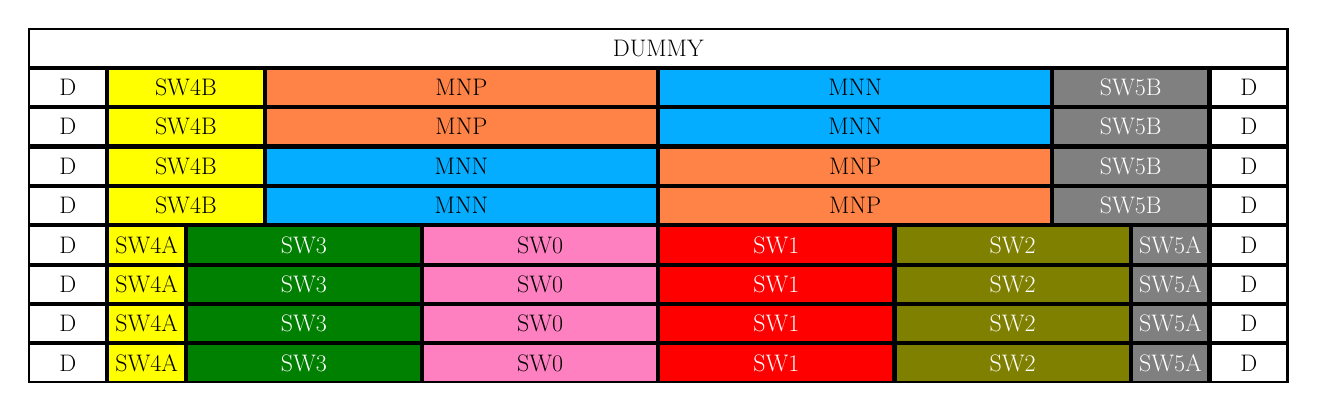
\begin{tikzpicture}[scale=0.5, transform shape]
		% Paths, nodes and wires:
		\node[shape=rectangle, fill={rgb,255:red,255;green,131;blue,70}, draw, line width=1pt, minimum width=9.965cm, minimum height=0.965cm] at (-5, 7.5){} node[anchor=center, align=center, text width=9.577cm, inner sep=6pt] at (-5, 7.5){\LARGE MNP};
		\node[shape=rectangle, fill={rgb,255:red,4;green,173;blue,255}, draw, line width=1pt, minimum width=9.965cm, minimum height=0.965cm] at (5, 7.5){} node[anchor=center, align=center, text width=9.577cm, inner sep=6pt] at (5, 7.5){\LARGE MNN};
		\node[shape=rectangle, fill={rgb,255:red,255;green,131;blue,70}, draw, line width=1pt, minimum width=9.965cm, minimum height=0.965cm] at (-5, 6.5){} node[anchor=center, align=center, text width=9.577cm, inner sep=6pt] at (-5, 6.5){\LARGE MNP};
		\node[shape=rectangle, fill={rgb,255:red,255;green,131;blue,70}, draw, line width=1pt, minimum width=9.965cm, minimum height=0.965cm] at (5, 5.5){} node[anchor=center, align=center, text width=9.577cm, inner sep=6pt] at (5, 5.5){\LARGE MNP};
		\node[shape=rectangle, fill={rgb,255:red,255;green,131;blue,70}, draw, line width=1pt, minimum width=9.965cm, minimum height=0.965cm] at (5, 4.5){} node[anchor=center, align=center, text width=9.577cm, inner sep=6pt] at (5, 4.5){\LARGE MNP};
		\node[shape=rectangle, fill={rgb,255:red,4;green,173;blue,255}, draw, line width=1pt, minimum width=9.965cm, minimum height=0.965cm] at (5, 6.5){} node[anchor=center, align=center, text width=9.577cm, inner sep=6pt] at (5, 6.5){\LARGE MNN};
		\node[shape=rectangle, fill={rgb,255:red,4;green,173;blue,255}, draw, line width=1pt, minimum width=9.965cm, minimum height=0.965cm] at (-5, 5.5){} node[anchor=center, align=center, text width=9.577cm, inner sep=6pt] at (-5, 5.5){\LARGE MNN};
		\node[shape=rectangle, fill={rgb,255:red,4;green,173;blue,255}, draw, line width=1pt, minimum width=9.965cm, minimum height=0.965cm] at (-5, 4.5){} node[anchor=center, align=center, text width=9.577cm, inner sep=6pt] at (-5, 4.5){\LARGE MNN};
		\node[shape=rectangle, fill={rgb,255:red,255;green,255;blue,0}, draw, line width=1pt, minimum width=3.965cm, minimum height=0.965cm] at (-12, 7.5){} node[anchor=center, align=center, text width=3.577cm, inner sep=6pt] at (-12, 7.5){\LARGE SW4B};
		\node[shape=rectangle, fill={rgb,255:red,255;green,255;blue,0}, draw, line width=1pt, minimum width=1.965cm, minimum height=0.965cm] at (-13, 3.5){} node[anchor=center, align=center, text width=1.577cm, inner sep=6pt] at (-13, 3.5){\LARGE SW4A};
		\node[shape=rectangle, fill={rgb,255:red,255;green,255;blue,0}, draw, line width=1pt, minimum width=1.965cm, minimum height=0.965cm] at (-13, 2.5){} node[anchor=center, align=center, text width=1.577cm, inner sep=6pt] at (-13, 2.5){\LARGE SW4A};
		\node[shape=rectangle, fill={rgb,255:red,255;green,255;blue,0}, draw, line width=1pt, minimum width=1.965cm, minimum height=0.965cm] at (-13, 1.5){} node[anchor=center, align=center, text width=1.577cm, inner sep=6pt] at (-13, 1.5){\LARGE SW4A};
		\node[shape=rectangle, fill={rgb,255:red,255;green,255;blue,0}, draw, line width=1pt, minimum width=1.965cm, minimum height=0.965cm] at (-13, 0.5){} node[anchor=center, align=center, text width=1.577cm, inner sep=6pt] at (-13, 0.5){\LARGE SW4A};
		\node[shape=rectangle, fill={rgb,255:red,255;green,255;blue,0}, draw, line width=1pt, minimum width=3.965cm, minimum height=0.965cm] at (-12, 6.5){} node[anchor=center, align=center, text width=3.577cm, inner sep=6pt] at (-12, 6.5){\LARGE SW4B};
		\node[shape=rectangle, fill={rgb,255:red,255;green,255;blue,0}, draw, line width=1pt, minimum width=3.965cm, minimum height=0.965cm] at (-12, 5.5){} node[anchor=center, align=center, text width=3.577cm, inner sep=6pt] at (-12, 5.5){\LARGE SW4B};
		\node[shape=rectangle, fill={rgb,255:red,255;green,255;blue,0}, draw, line width=1pt, minimum width=3.965cm, minimum height=0.965cm] at (-12, 4.5){} node[anchor=center, align=center, text width=3.577cm, inner sep=6pt] at (-12, 4.5){\LARGE SW4B};
		\node[shape=rectangle, fill={rgb,255:red,0;green,128;blue,0}, draw, line width=1pt, minimum width=5.965cm, minimum height=0.965cm] at (-9, 2.5){} node[anchor=center, align=center, text width=5.577cm, inner sep=6pt] at (-9, 2.5){\textcolor{rgb,255:red,255;green,255;blue,255}{\LARGE SW3\\}};
		\node[shape=rectangle, fill={rgb,255:red,0;green,128;blue,0}, draw, line width=1pt, minimum width=5.965cm, minimum height=0.965cm] at (-9, 3.5){} node[anchor=center, align=center, text width=5.577cm, inner sep=6pt] at (-9, 3.5){\textcolor{rgb,255:red,255;green,255;blue,255}{\LARGE SW3\\}};
		\node[shape=rectangle, fill={rgb,255:red,0;green,128;blue,0}, draw, line width=1pt, minimum width=5.965cm, minimum height=0.965cm] at (-9, 0.5){} node[anchor=center, align=center, text width=5.577cm, inner sep=6pt] at (-9, 0.5){\textcolor{rgb,255:red,255;green,255;blue,255}{\LARGE SW3\\}};
		\node[shape=rectangle, fill={rgb,255:red,0;green,128;blue,0}, draw, line width=1pt, minimum width=5.965cm, minimum height=0.965cm] at (-9, 1.5){} node[anchor=center, align=center, text width=5.577cm, inner sep=6pt] at (-9, 1.5){\textcolor{rgb,255:red,255;green,255;blue,255}{\LARGE SW3\\}};
		\node[shape=rectangle, fill={rgb,255:red,255;green,128;blue,192}, draw, line width=1pt, minimum width=5.965cm, minimum height=0.965cm] at (-3, 3.5){} node[anchor=center, align=center, text width=5.577cm, inner sep=6pt] at (-3, 3.5){\LARGE SW0\\};
		\node[shape=rectangle, fill={rgb,255:red,255;green,128;blue,192}, draw, line width=1pt, minimum width=5.965cm, minimum height=0.965cm] at (-3, 2.5){} node[anchor=center, align=center, text width=5.577cm, inner sep=6pt] at (-3, 2.5){\LARGE SW0\\};
		\node[shape=rectangle, fill={rgb,255:red,255;green,128;blue,192}, draw, line width=1pt, minimum width=5.965cm, minimum height=0.965cm] at (-3, 1.5){} node[anchor=center, align=center, text width=5.577cm, inner sep=6pt] at (-3, 1.5){\LARGE SW0\\};
		\node[shape=rectangle, fill={rgb,255:red,255;green,128;blue,192}, draw, line width=1pt, minimum width=5.965cm, minimum height=0.965cm] at (-3, 0.5){} node[anchor=center, align=center, text width=5.577cm, inner sep=6pt] at (-3, 0.5){\LARGE SW0\\};
		\node[shape=rectangle, fill={rgb,255:red,255;green,0;blue,0}, draw, line width=1pt, minimum width=5.965cm, minimum height=0.965cm] at (3, 3.5){} node[anchor=center, align=center, text width=5.577cm, inner sep=6pt] at (3, 3.5){\textcolor{rgb,255:red,255;green,255;blue,255}{\LARGE SW1\\}};
		\node[shape=rectangle, fill={rgb,255:red,255;green,0;blue,0}, draw, line width=1pt, minimum width=5.965cm, minimum height=0.965cm] at (3, 2.5){} node[anchor=center, align=center, text width=5.577cm, inner sep=6pt] at (3, 2.5){\textcolor{rgb,255:red,255;green,255;blue,255}{\LARGE SW1\\}};
		\node[shape=rectangle, fill={rgb,255:red,255;green,0;blue,0}, draw, line width=1pt, minimum width=5.965cm, minimum height=0.965cm] at (3, 1.5){} node[anchor=center, align=center, text width=5.577cm, inner sep=6pt] at (3, 1.5){\textcolor{rgb,255:red,255;green,255;blue,255}{\LARGE SW1\\}};
		\node[shape=rectangle, fill={rgb,255:red,255;green,0;blue,0}, draw, line width=1pt, minimum width=5.965cm, minimum height=0.965cm] at (3, 0.5){} node[anchor=center, align=center, text width=5.577cm, inner sep=6pt] at (3, 0.5){\textcolor{rgb,255:red,255;green,255;blue,255}{\LARGE SW1\\}};
		\node[shape=rectangle, fill={rgb,255:red,128;green,128;blue,0}, draw, line width=1pt, minimum width=5.965cm, minimum height=0.965cm] at (9, 3.5){} node[anchor=center, align=center, text width=5.577cm, inner sep=6pt] at (9, 3.5){\textcolor{rgb,255:red,255;green,255;blue,255}{\LARGE SW2\\}};
		\node[shape=rectangle, fill={rgb,255:red,128;green,128;blue,0}, draw, line width=1pt, minimum width=5.965cm, minimum height=0.965cm] at (9, 2.5){} node[anchor=center, align=center, text width=5.577cm, inner sep=6pt] at (9, 2.5){\textcolor{rgb,255:red,255;green,255;blue,255}{\LARGE SW2\\}};
		\node[shape=rectangle, fill={rgb,255:red,128;green,128;blue,0}, draw, line width=1pt, minimum width=5.965cm, minimum height=0.965cm] at (9, 1.5){} node[anchor=center, align=center, text width=5.577cm, inner sep=6pt] at (9, 1.5){\textcolor{rgb,255:red,255;green,255;blue,255}{\LARGE SW2\\}};
		\node[shape=rectangle, fill={rgb,255:red,128;green,128;blue,0}, draw, line width=1pt, minimum width=5.965cm, minimum height=0.965cm] at (9, 0.5){} node[anchor=center, align=center, text width=5.577cm, inner sep=6pt] at (9, 0.5){\textcolor{rgb,255:red,255;green,255;blue,255}{\LARGE SW2\\}};
		\node[shape=rectangle, fill={rgb,255:red,128;green,128;blue,128}, draw, line width=1pt, minimum width=3.965cm, minimum height=0.965cm] at (12, 4.5){} node[anchor=center, align=center, text width=3.577cm, inner sep=6pt] at (12, 4.5){\textcolor{rgb,255:red,255;green,255;blue,255}{\LARGE SW5B}};
		\node[shape=rectangle, fill={rgb,255:red,128;green,128;blue,128}, draw, line width=1pt, minimum width=1.965cm, minimum height=0.965cm] at (13, 3.5){} node[anchor=center, align=center, text width=1.577cm, inner sep=6pt] at (13, 3.5){\textcolor{rgb,255:red,255;green,255;blue,255}{\LARGE SW5A}};
		\node[shape=rectangle, fill={rgb,255:red,128;green,128;blue,128}, draw, line width=1pt, minimum width=3.965cm, minimum height=0.965cm] at (12, 5.5){} node[anchor=center, align=center, text width=3.577cm, inner sep=6pt] at (12, 5.5){\textcolor{rgb,255:red,255;green,255;blue,255}{\LARGE SW5B}};
		\node[shape=rectangle, fill={rgb,255:red,128;green,128;blue,128}, draw, line width=1pt, minimum width=3.965cm, minimum height=0.965cm] at (12, 6.5){} node[anchor=center, align=center, text width=3.577cm, inner sep=6pt] at (12, 6.5){\textcolor{rgb,255:red,255;green,255;blue,255}{\LARGE SW5B}};
		\node[shape=rectangle, fill={rgb,255:red,128;green,128;blue,128}, draw, line width=1pt, minimum width=3.965cm, minimum height=0.965cm] at (12, 7.5){} node[anchor=center, align=center, text width=3.577cm, inner sep=6pt] at (12, 7.5){\textcolor{rgb,255:red,255;green,255;blue,255}{\LARGE SW5B}};
		\node[shape=rectangle, fill={rgb,255:red,128;green,128;blue,128}, draw, line width=1pt, minimum width=1.965cm, minimum height=0.965cm] at (13, 2.5){} node[anchor=center, align=center, text width=1.577cm, inner sep=6pt] at (13, 2.5){\textcolor{rgb,255:red,255;green,255;blue,255}{\LARGE SW5A}};
		\node[shape=rectangle, fill={rgb,255:red,128;green,128;blue,128}, draw, line width=1pt, minimum width=1.965cm, minimum height=0.965cm] at (13, 1.5){} node[anchor=center, align=center, text width=1.577cm, inner sep=6pt] at (13, 1.5){\textcolor{rgb,255:red,255;green,255;blue,255}{\LARGE SW5A}};
		\node[shape=rectangle, fill={rgb,255:red,128;green,128;blue,128}, draw, line width=1pt, minimum width=1.965cm, minimum height=0.965cm] at (13, 0.5){} node[anchor=center, align=center, text width=1.577cm, inner sep=6pt] at (13, 0.5){\textcolor{rgb,255:red,255;green,255;blue,255}{\LARGE SW5A}};
		\node[shape=rectangle, fill={rgb,255:red,255;green,255;blue,255}, draw, line width=1pt, minimum width=1.965cm, minimum height=0.965cm] at (-15, 7.5){} node[anchor=center, align=center, text width=1.577cm, inner sep=6pt] at (-15, 7.5){\LARGE D};
		\node[shape=rectangle, fill={rgb,255:red,255;green,255;blue,255}, draw, line width=1pt, minimum width=1.965cm, minimum height=0.965cm] at (-15, 6.5){} node[anchor=center, align=center, text width=1.577cm, inner sep=6pt] at (-15, 6.5){\LARGE D};
		\node[shape=rectangle, fill={rgb,255:red,255;green,255;blue,255}, draw, line width=1pt, minimum width=1.965cm, minimum height=0.965cm] at (-15, 5.5){} node[anchor=center, align=center, text width=1.577cm, inner sep=6pt] at (-15, 5.5){\LARGE D};
		\node[shape=rectangle, fill={rgb,255:red,255;green,255;blue,255}, draw, line width=1pt, minimum width=1.965cm, minimum height=0.965cm] at (-15, 4.5){} node[anchor=center, align=center, text width=1.577cm, inner sep=6pt] at (-15, 4.5){\LARGE D};
		\node[shape=rectangle, fill={rgb,255:red,255;green,255;blue,255}, draw, line width=1pt, minimum width=1.965cm, minimum height=0.965cm] at (-15, 3.5){} node[anchor=center, align=center, text width=1.577cm, inner sep=6pt] at (-15, 3.5){\LARGE D};
		\node[shape=rectangle, fill={rgb,255:red,255;green,255;blue,255}, draw, line width=1pt, minimum width=1.965cm, minimum height=0.965cm] at (-15, 2.5){} node[anchor=center, align=center, text width=1.577cm, inner sep=6pt] at (-15, 2.5){\LARGE D};
		\node[shape=rectangle, fill={rgb,255:red,255;green,255;blue,255}, draw, line width=1pt, minimum width=1.965cm, minimum height=0.965cm] at (-15, 1.5){} node[anchor=center, align=center, text width=1.577cm, inner sep=6pt] at (-15, 1.5){\LARGE D};
		\node[shape=rectangle, fill={rgb,255:red,255;green,255;blue,255}, draw, line width=1pt, minimum width=1.965cm, minimum height=0.965cm] at (-15, 0.5){} node[anchor=center, align=center, text width=1.577cm, inner sep=6pt] at (-15, 0.5){\LARGE D};
		\node[shape=rectangle, fill={rgb,255:red,255;green,255;blue,255}, draw, line width=1pt, minimum width=1.965cm, minimum height=0.965cm] at (15, 7.5){} node[anchor=center, align=center, text width=1.577cm, inner sep=6pt] at (15, 7.5){\LARGE D};
		\node[shape=rectangle, fill={rgb,255:red,255;green,255;blue,255}, draw, line width=1pt, minimum width=1.965cm, minimum height=0.965cm] at (15, 6.5){} node[anchor=center, align=center, text width=1.577cm, inner sep=6pt] at (15, 6.5){\LARGE D};
		\node[shape=rectangle, fill={rgb,255:red,255;green,255;blue,255}, draw, line width=1pt, minimum width=1.965cm, minimum height=0.965cm] at (15, 5.5){} node[anchor=center, align=center, text width=1.577cm, inner sep=6pt] at (15, 5.5){\LARGE D};
		\node[shape=rectangle, fill={rgb,255:red,255;green,255;blue,255}, draw, line width=1pt, minimum width=1.965cm, minimum height=0.965cm] at (15, 4.5){} node[anchor=center, align=center, text width=1.577cm, inner sep=6pt] at (15, 4.5){\LARGE D};
		\node[shape=rectangle, fill={rgb,255:red,255;green,255;blue,255}, draw, line width=1pt, minimum width=1.965cm, minimum height=0.965cm] at (15, 3.5){} node[anchor=center, align=center, text width=1.577cm, inner sep=6pt] at (15, 3.5){\LARGE D};
		\node[shape=rectangle, fill={rgb,255:red,255;green,255;blue,255}, draw, line width=1pt, minimum width=1.965cm, minimum height=0.965cm] at (15, 2.5){} node[anchor=center, align=center, text width=1.577cm, inner sep=6pt] at (15, 2.5){\LARGE D};
		\node[shape=rectangle, fill={rgb,255:red,255;green,255;blue,255}, draw, line width=1pt, minimum width=1.965cm, minimum height=0.965cm] at (15, 1.5){} node[anchor=center, align=center, text width=1.577cm, inner sep=6pt] at (15, 1.5){\LARGE D};
		\node[shape=rectangle, fill={rgb,255:red,255;green,255;blue,255}, draw, line width=1pt, minimum width=1.965cm, minimum height=0.965cm] at (15, 0.5){} node[anchor=center, align=center, text width=1.577cm, inner sep=6pt] at (15, 0.5){\LARGE D};
		\node[shape=rectangle, fill={rgb,255:red,255;green,255;blue,255}, draw, line width=1pt, minimum width=31.965cm, minimum height=0.965cm] at (0, 8.5){} node[anchor=center, align=center, text width=31.577cm, inner sep=6pt] at (0, 8.5){\LARGE DUMMY};
	\end{tikzpicture}
	}
	\caption{\ac{RVT} devices floorplan}\label{fig:RVT_floorplan}
\end{figure}

As mentioned above, the addition of the switches to the floorplan was done with a focus on layout geometry and area. To this end, measuring the floorplan width with finger counts instead of physical dimensions makes it easier to find the most optimal arrangement that results in a balanced tradeoff between area and geometry. The following considerations were taken into account when deciding how to position the current mirror switches:

\begin{enumerate}
	\item The even number of switching devices makes it possible to split them into equal groups and mirror them across the vertical symmetry axis of the differential pair, resulting in a symmetrical arrangement of all active devices.
	\item There is still a need for dummy devices to be added to the side edges of the floorplan to keep the standard cell abuttable, examplified in Figure~\ref{fig:abut_cells_example}. These dummy devices will be used to connect adjacent cells to VSS, and isolate the terminal of the active switching devices, which is only possible if these dummy devices have at least two fingers.
	\item Each switch has 24 fingers, which makes it reasonable to split in even multiples of 6 or 4 
	\item The considerably longer width of the current mirror devices has to be accounted for when deciding how the switches will be split, since the driver is floorplanned to have the tap units horizontally abuttable. If the differential pair floorplan is to narrow, this will be amplified by the current mirror bank and result in a narrow standard cell, making local cell routing and matching of the mirror devices more difficult.
\end{enumerate}
 
The final floorplan of the \ac{RVT} devices, shown in Figure~\ref{fig:RVT_floorplan}, has a width of 32 fingers. Devices SW0, SW1, SW2 and SW3 have 6 fingers each, with multiplicity of 4. In order to occupy the lowest area possible, devices SW4 and SW5 are split into two sub devices, SW4A and SW5A, with 2 fingers and multiplicity of 4, and SW4B and SW5B, with 4 fingers and multiplicity of 4. This arrangement allowed for the minimum width of 32 fingers to be realized, which is just enough width for the current mirror \ac{SLVT} floorplan to be designed without leaving too much unused area.

\begin{figure}[h]
	\resizebox{0.75\textwidth}{!}{
	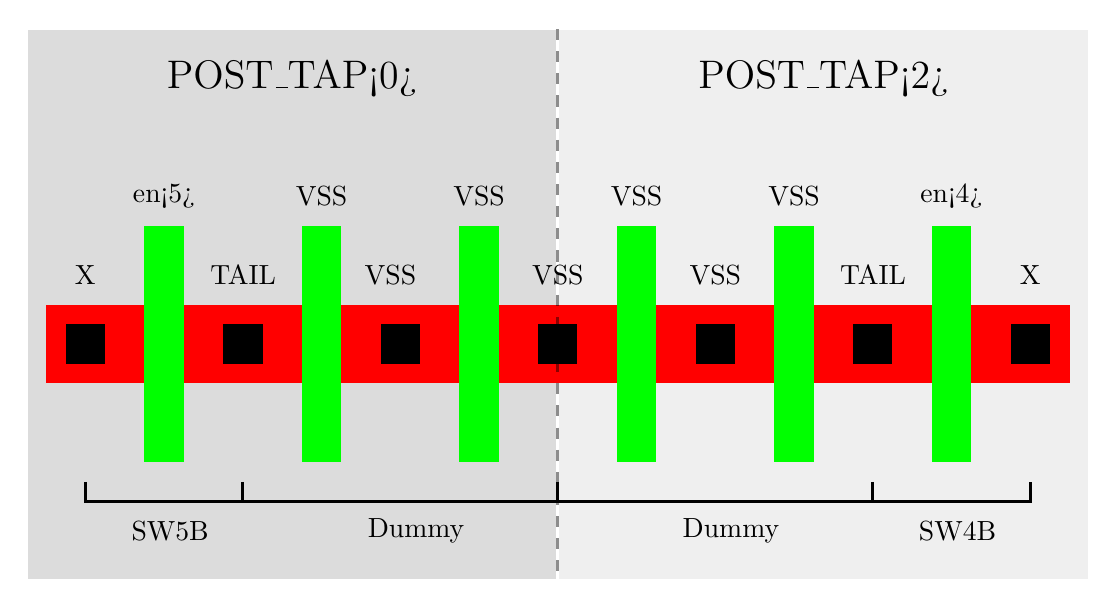
\begin{tikzpicture}[transform shape]
		% Paths, nodes and wires:
		\node[shape=rectangle, fill={rgb,255:red,128;green,128;blue,128}, fill opacity=0.13, minimum width=6.715cm, minimum height=6.965cm] at (10.125, 3.5){};
		\node[shape=rectangle, fill={rgb,255:red,128;green,128;blue,128}, fill opacity=0.28, minimum width=6.715cm, minimum height=6.965cm] at (3.375, 3.5){};
		\node[shape=rectangle, fill={rgb,255:red,255;green,0;blue,0}, draw={rgb,255:red,255;green,0;blue,0}, line width=1pt, minimum width=12.965cm, minimum height=0.965cm] at (6.75, 3){};
		\node[shape=rectangle, fill={rgb,255:red,0;green,0;blue,0}, draw, line width=1pt, minimum width=0.465cm, minimum height=0.465cm] at (6.75, 3){};
		\node[shape=rectangle, fill={rgb,255:red,0;green,0;blue,0}, draw, line width=1pt, minimum width=0.465cm, minimum height=0.465cm] at (8.75, 3){};
		\node[shape=rectangle, fill={rgb,255:red,0;green,255;blue,0}, draw={rgb,255:red,0;green,255;blue,0}, line width=1pt, minimum width=0.465cm, minimum height=2.965cm] at (7.75, 3){};
		\node[shape=rectangle, fill={rgb,255:red,0;green,255;blue,0}, draw={rgb,255:red,0;green,255;blue,0}, line width=1pt, minimum width=0.465cm, minimum height=2.965cm] at (9.75, 3){};
		\node[shape=rectangle, fill={rgb,255:red,0;green,0;blue,0}, draw, line width=1pt, minimum width=0.465cm, minimum height=0.465cm] at (10.75, 3){};
		\node[shape=rectangle, minimum width=1.215cm, minimum height=0.715cm] at (7.75, 4.875){} node[anchor=center, align=center, text width=0.827cm, inner sep=6pt] at (7.75, 4.875){VSS};
		\node[shape=rectangle, minimum width=1.215cm, minimum height=0.715cm] at (9.75, 4.875){} node[anchor=center, align=center, text width=0.827cm, inner sep=6pt] at (9.75, 4.875){VSS};
		\node[shape=rectangle, fill={rgb,255:red,0;green,255;blue,0}, draw={rgb,255:red,0;green,255;blue,0}, line width=1pt, minimum width=0.465cm, minimum height=2.965cm] at (11.75, 3){};
		\node[shape=rectangle, fill={rgb,255:red,0;green,0;blue,0}, draw, line width=1pt, minimum width=0.465cm, minimum height=0.465cm] at (12.75, 3){};
		\node[shape=rectangle, fill={rgb,255:red,0;green,255;blue,0}, draw={rgb,255:red,0;green,255;blue,0}, line width=1pt, minimum width=0.465cm, minimum height=2.965cm] at (5.75, 3){};
		\node[shape=rectangle, fill={rgb,255:red,0;green,0;blue,0}, draw, line width=1pt, minimum width=0.465cm, minimum height=0.465cm] at (4.75, 3){};
		\node[shape=rectangle, minimum width=1.215cm, minimum height=0.715cm] at (8.75, 3.875){} node[anchor=center, align=center, text width=0.827cm, inner sep=6pt] at (8.75, 3.875){VSS};
		\node[shape=rectangle, minimum width=1.215cm, minimum height=0.715cm] at (10.75, 3.875){} node[anchor=center, align=center, text width=0.827cm, inner sep=6pt] at (10.75, 3.875){TAIL};
		\node[shape=rectangle, minimum width=1.215cm, minimum height=0.715cm] at (11.75, 4.875){} node[anchor=center, align=center, text width=0.827cm, inner sep=6pt] at (11.75, 4.875){en<4>};
		\node[shape=rectangle, minimum width=1.215cm, minimum height=0.715cm] at (12.75, 3.875){} node[anchor=center, align=center, text width=0.827cm, inner sep=6pt] at (12.75, 3.875){X};
		\draw[draw opacity=0.45, line width=1pt, dash pattern={on 4pt off 4pt}] (6.75, 7) -- (6.75, 0);
		\node[shape=rectangle, minimum width=1.215cm, minimum height=0.715cm] at (5.75, 4.875){} node[anchor=center, align=center, text width=0.827cm, inner sep=6pt] at (5.75, 4.875){VSS};
		\node[shape=rectangle, fill={rgb,255:red,0;green,255;blue,0}, draw={rgb,255:red,0;green,255;blue,0}, line width=1pt, minimum width=0.465cm, minimum height=2.965cm] at (3.75, 3){};
		\node[shape=rectangle, minimum width=1.215cm, minimum height=0.715cm] at (3.75, 4.875){} node[anchor=center, align=center, text width=0.827cm, inner sep=6pt] at (3.75, 4.875){VSS};
		\node[shape=rectangle, fill={rgb,255:red,0;green,0;blue,0}, draw, line width=1pt, minimum width=0.465cm, minimum height=0.465cm] at (2.75, 3){};
		\node[shape=rectangle, minimum width=1.215cm, minimum height=0.715cm] at (4.625, 3.875){} node[anchor=center, align=center, text width=0.827cm, inner sep=6pt] at (4.625, 3.875){VSS};
		\node[shape=rectangle, minimum width=1.215cm, minimum height=0.715cm] at (2.75, 3.875){} node[anchor=center, align=center, text width=0.827cm, inner sep=6pt] at (2.75, 3.875){TAIL};
		\node[shape=rectangle, fill={rgb,255:red,0;green,0;blue,0}, draw, line width=1pt, minimum width=0.465cm, minimum height=0.465cm] at (0.75, 3){};
		\node[shape=rectangle, fill={rgb,255:red,0;green,255;blue,0}, draw={rgb,255:red,0;green,255;blue,0}, line width=1pt, minimum width=0.465cm, minimum height=2.965cm] at (1.75, 3){};
		\node[shape=rectangle, minimum width=1.215cm, minimum height=0.715cm] at (1.75, 4.875){} node[anchor=center, align=center, text width=0.827cm, inner sep=6pt] at (1.75, 4.875){en<5>};
		\node[shape=rectangle, minimum width=1.215cm, minimum height=0.715cm] at (0.75, 3.875){} node[anchor=center, align=center, text width=0.827cm, inner sep=6pt] at (0.75, 3.875){X};
		\node[shape=rectangle, minimum width=1.215cm, minimum height=0.715cm] at (6.75, 3.875){} node[anchor=center, align=center, text width=0.827cm, inner sep=6pt] at (6.75, 3.875){VSS};
		\draw[line width=1pt] (2.75, 1.25) -- (2.75, 1) -- (6.75, 1) -| (6.75, 1.25);
		\node[shape=rectangle, minimum width=1.215cm, minimum height=0.715cm] at (4.75, 0.625){} node[anchor=center, align=center, text width=0.827cm, inner sep=6pt] at (4.75, 0.625){Dummy};
		\draw[line width=1pt] (6.75, 1.25) -- (6.75, 1) -| (10.75, 1) -| (10.75, 1.25);
		\node[shape=rectangle, minimum width=1.215cm, minimum height=0.715cm] at (8.75, 0.625){} node[anchor=center, align=center, text width=0.827cm, inner sep=6pt] at (8.75, 0.625){Dummy};
		\draw[line width=1pt] (0.75, 1.25) -- (0.75, 1) -| (2.75, 1) -| (2.75, 1.25);
		\node[shape=rectangle, minimum width=1.215cm, minimum height=0.715cm] at (1.75, 0.625){} node[anchor=center, align=center, text width=0.827cm, inner sep=6pt] at (1.75, 0.625){SW5B};
		\draw[line width=1pt] (10.75, 1.25) -- (10.75, 1) -- (12.75, 1) -| (12.75, 1.25);
		\node[shape=rectangle, minimum width=1.215cm, minimum height=0.715cm] at (11.75, 0.625){} node[anchor=center, align=center, text width=0.827cm, inner sep=6pt] at (11.75, 0.625){SW4B};
		\node[shape=rectangle, minimum width=4.215cm, minimum height=0.715cm] at (3.375, 6.375){} node[anchor=center, align=center, text width=3.827cm, inner sep=6pt] at (3.375, 6.375){\Large POST\_TAP<0>};
		\node[shape=rectangle, minimum width=4.215cm, minimum height=0.715cm] at (10.125, 6.375){} node[anchor=center, align=center, text width=3.827cm, inner sep=6pt] at (10.125, 6.375){\Large POST\_TAP<2>};
	\end{tikzpicture}
	}
	\caption{Example of adjacent cell abutting using dummies}\label{fig:abut_cells_example}
\end{figure}

%The current mirror bank floorplan was designed only after the differential pair floorplan had been established, reflecting the relative criticality of the two device groups: since the differential pair is the most sensitive part of the tap unit to matching, its floorplan was prioritized, while the current mirror bank, being comparatively less sensitive to matching, was fit around the constraints already imposed by the differential pair.

The current-mirror devices were likewise arranged in a common-centroid configuration. Unlike the differential pair, however, this choice was not driven primarily by the need to compensate for process gradients, but rather by the geometric constraints imposed by the width of the \ac{RVT} floorplan. Within the available cell width, a conventional interdigitated arrangement would have resulted in an impractical aspect ratio and insufficient routing space. The common-centroid arrangement therefore provided a compact solution while preserving symmetry and adequate matching between the current-mirror devices.

Each logical current-mirror device is implemented using 30 identical two-finger sub-devices, corresponding to the $\mathrm{n_f=2}$ and $\mathrm{m=30}$ configuration listed in Table~\ref{tab:tap_unit_device_parameters}. These sub-devices are distributed symmetrically throughout the \ac{SLVT} floorplan, shown in Figure~\ref{fig:SLVT_floorplan}. Dummy devices were inserted between groups of active mirror devices to provide additional routing space for the connections between the enable switches and their corresponding current mirrors. Additional dummy devices were placed along the outer edges of the floorplan to maintain a uniform device environment, reduce edge-dependent effects, and preserve symmetry. Since all active current-mirror devices must remain in saturation and are biased by the common replica-based reference generator, maintaining similar physical surroundings and operating conditions among the mirror devices is important for limiting systematic current mismatch.

With the \ac{RVT} and \ac{SLVT} device floorplans defined, the PMOS termination-switch devices were then arranged. These devices perform a switching function analogous to that of the \ac{RVT} NMOS current-mirror switches, but are used to enable or disable the 1~\unit{\kilo\ohm} resistor branches that form the configurable on-die termination network. Each PMOS switch is implemented with 16 fingers and a multiplicity of five, resulting in a total effective finger count of 80. Because these devices operate primarily as switches for passive termination elements, their matching requirements are less stringent than those of the differential pair or current-mirror devices. The PMOS floorplan was therefore optimized primarily for area efficiency and compatibility with the standard-cell geometry. Since the PMOS devices use the same channel length as the \ac{RVT} NMOS switches, their arrangement could be designed to match the width of the \ac{RVT} floorplan, avoiding unused lateral area and maintaining a uniform cell boundary for abutment.

\begin{figure}[h]
    \centering
	\resizebox{0.6\textwidth}{!}{
	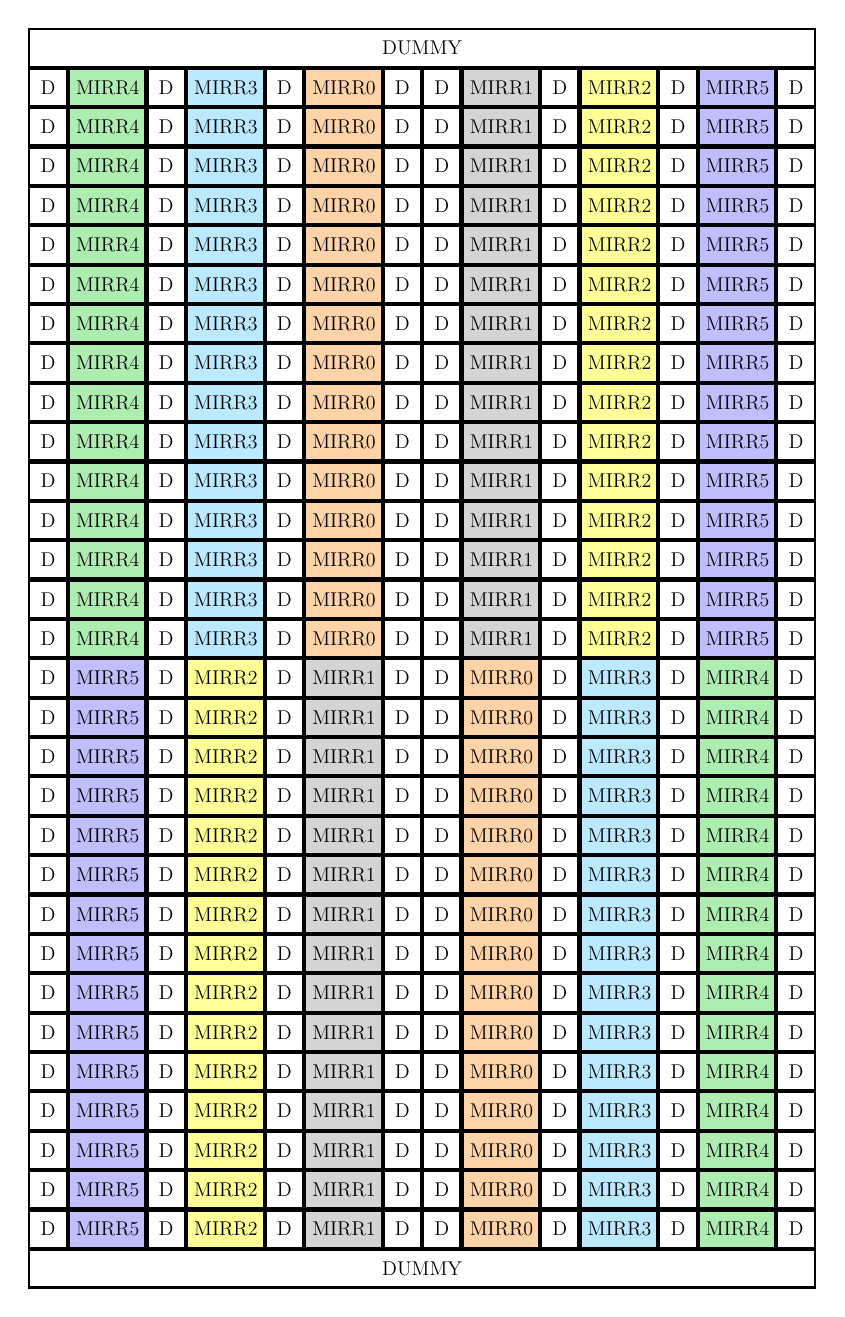
\begin{tikzpicture}[scale=0.5, transform shape]
		% Paths, nodes and wires:
		\node[shape=rectangle, fill={rgb,255:red,255;green,211;blue,168}, draw, line width=1pt, minimum width=1.965cm, minimum height=0.965cm] at (-2, 30.5){} node[anchor=center, align=center, text width=1.577cm, inner sep=6pt] at (-2, 30.5){\Large MIRR0};
		\node[shape=rectangle, fill={rgb,255:red,212;green,212;blue,212}, draw, line width=1pt, minimum width=1.965cm, minimum height=0.965cm] at (2, 30.5){} node[anchor=center, align=center, text width=1.577cm, inner sep=6pt] at (2, 30.5){\Large MIRR1};
		\node[shape=rectangle, fill={rgb,255:red,255;green,255;blue,151}, draw, line width=1pt, minimum width=1.965cm, minimum height=0.965cm] at (5, 30.5){} node[anchor=center, align=center, text width=1.577cm, inner sep=6pt] at (5, 30.5){\Large MIRR2};
		\node[shape=rectangle, fill={rgb,255:red,187;green,233;blue,255}, draw, line width=1pt, minimum width=1.965cm, minimum height=0.965cm] at (-5, 30.5){} node[anchor=center, align=center, text width=1.577cm, inner sep=6pt] at (-5, 30.5){\Large MIRR3};
		\node[shape=rectangle, fill={rgb,255:red,173;green,237;blue,176}, draw, line width=1pt, minimum width=1.965cm, minimum height=0.965cm] at (-8, 27.5){} node[anchor=center, align=center, text width=1.577cm, inner sep=6pt] at (-8, 27.5){\Large MIRR4};
		\node[shape=rectangle, fill={rgb,255:red,191;green,191;blue,255}, draw, line width=1pt, minimum width=1.965cm, minimum height=0.965cm] at (8, 30.5){} node[anchor=center, align=center, text width=1.577cm, inner sep=6pt] at (8, 30.5){\Large MIRR5};
		\node[shape=rectangle, fill={rgb,255:red,173;green,237;blue,176}, draw, line width=1pt, minimum width=1.965cm, minimum height=0.965cm] at (-8, 26.5){} node[anchor=center, align=center, text width=1.577cm, inner sep=6pt] at (-8, 26.5){\Large MIRR4};
		\node[shape=rectangle, fill={rgb,255:red,173;green,237;blue,176}, draw, line width=1pt, minimum width=1.965cm, minimum height=0.965cm] at (-8, 25.5){} node[anchor=center, align=center, text width=1.577cm, inner sep=6pt] at (-8, 25.5){\Large MIRR4};
		\node[shape=rectangle, fill={rgb,255:red,173;green,237;blue,176}, draw, line width=1pt, minimum width=1.965cm, minimum height=0.965cm] at (-8, 24.5){} node[anchor=center, align=center, text width=1.577cm, inner sep=6pt] at (-8, 24.5){\Large MIRR4};
		\node[shape=rectangle, fill={rgb,255:red,173;green,237;blue,176}, draw, line width=1pt, minimum width=1.965cm, minimum height=0.965cm] at (-8, 23.5){} node[anchor=center, align=center, text width=1.577cm, inner sep=6pt] at (-8, 23.5){\Large MIRR4};
		\node[shape=rectangle, fill={rgb,255:red,173;green,237;blue,176}, draw, line width=1pt, minimum width=1.965cm, minimum height=0.965cm] at (-8, 22.5){} node[anchor=center, align=center, text width=1.577cm, inner sep=6pt] at (-8, 22.5){\Large MIRR4};
		\node[shape=rectangle, fill={rgb,255:red,173;green,237;blue,176}, draw, line width=1pt, minimum width=1.965cm, minimum height=0.965cm] at (-8, 21.5){} node[anchor=center, align=center, text width=1.577cm, inner sep=6pt] at (-8, 21.5){\Large MIRR4};
		\node[shape=rectangle, fill={rgb,255:red,173;green,237;blue,176}, draw, line width=1pt, minimum width=1.965cm, minimum height=0.965cm] at (-8, 20.5){} node[anchor=center, align=center, text width=1.577cm, inner sep=6pt] at (-8, 20.5){\Large MIRR4};
		\node[shape=rectangle, fill={rgb,255:red,173;green,237;blue,176}, draw, line width=1pt, minimum width=1.965cm, minimum height=0.965cm] at (-8, 19.5){} node[anchor=center, align=center, text width=1.577cm, inner sep=6pt] at (-8, 19.5){\Large MIRR4};
		\node[shape=rectangle, fill={rgb,255:red,173;green,237;blue,176}, draw, line width=1pt, minimum width=1.965cm, minimum height=0.965cm] at (-8, 18.5){} node[anchor=center, align=center, text width=1.577cm, inner sep=6pt] at (-8, 18.5){\Large MIRR4};
		\node[shape=rectangle, fill={rgb,255:red,173;green,237;blue,176}, draw, line width=1pt, minimum width=1.965cm, minimum height=0.965cm] at (-8, 17.5){} node[anchor=center, align=center, text width=1.577cm, inner sep=6pt] at (-8, 17.5){\Large MIRR4};
		\node[shape=rectangle, fill={rgb,255:red,173;green,237;blue,176}, draw, line width=1pt, minimum width=1.965cm, minimum height=0.965cm] at (-8, 16.5){} node[anchor=center, align=center, text width=1.577cm, inner sep=6pt] at (-8, 16.5){\Large MIRR4};
		\node[shape=rectangle, fill={rgb,255:red,173;green,237;blue,176}, draw, line width=1pt, minimum width=1.965cm, minimum height=0.965cm] at (-8, 30.5){} node[anchor=center, align=center, text width=1.577cm, inner sep=6pt] at (-8, 30.5){\Large MIRR4};
		\node[shape=rectangle, fill={rgb,255:red,173;green,237;blue,176}, draw, line width=1pt, minimum width=1.965cm, minimum height=0.965cm] at (-8, 29.5){} node[anchor=center, align=center, text width=1.577cm, inner sep=6pt] at (-8, 29.5){\Large MIRR4};
		\node[shape=rectangle, fill={rgb,255:red,173;green,237;blue,176}, draw, line width=1pt, minimum width=1.965cm, minimum height=0.965cm] at (-8, 28.5){} node[anchor=center, align=center, text width=1.577cm, inner sep=6pt] at (-8, 28.5){\Large MIRR4};
		\node[shape=rectangle, fill={rgb,255:red,187;green,233;blue,255}, draw, line width=1pt, minimum width=1.965cm, minimum height=0.965cm] at (-5, 29.5){} node[anchor=center, align=center, text width=1.577cm, inner sep=6pt] at (-5, 29.5){\Large MIRR3};
		\node[shape=rectangle, fill={rgb,255:red,187;green,233;blue,255}, draw, line width=1pt, minimum width=1.965cm, minimum height=0.965cm] at (-5, 28.5){} node[anchor=center, align=center, text width=1.577cm, inner sep=6pt] at (-5, 28.5){\Large MIRR3};
		\node[shape=rectangle, fill={rgb,255:red,187;green,233;blue,255}, draw, line width=1pt, minimum width=1.965cm, minimum height=0.965cm] at (-5, 27.5){} node[anchor=center, align=center, text width=1.577cm, inner sep=6pt] at (-5, 27.5){\Large MIRR3};
		\node[shape=rectangle, fill={rgb,255:red,187;green,233;blue,255}, draw, line width=1pt, minimum width=1.965cm, minimum height=0.965cm] at (-5, 26.5){} node[anchor=center, align=center, text width=1.577cm, inner sep=6pt] at (-5, 26.5){\Large MIRR3};
		\node[shape=rectangle, fill={rgb,255:red,187;green,233;blue,255}, draw, line width=1pt, minimum width=1.965cm, minimum height=0.965cm] at (-5, 25.5){} node[anchor=center, align=center, text width=1.577cm, inner sep=6pt] at (-5, 25.5){\Large MIRR3};
		\node[shape=rectangle, fill={rgb,255:red,187;green,233;blue,255}, draw, line width=1pt, minimum width=1.965cm, minimum height=0.965cm] at (-5, 24.5){} node[anchor=center, align=center, text width=1.577cm, inner sep=6pt] at (-5, 24.5){\Large MIRR3};
		\node[shape=rectangle, fill={rgb,255:red,187;green,233;blue,255}, draw, line width=1pt, minimum width=1.965cm, minimum height=0.965cm] at (-5, 23.5){} node[anchor=center, align=center, text width=1.577cm, inner sep=6pt] at (-5, 23.5){\Large MIRR3};
		\node[shape=rectangle, fill={rgb,255:red,187;green,233;blue,255}, draw, line width=1pt, minimum width=1.965cm, minimum height=0.965cm] at (-5, 22.5){} node[anchor=center, align=center, text width=1.577cm, inner sep=6pt] at (-5, 22.5){\Large MIRR3};
		\node[shape=rectangle, fill={rgb,255:red,187;green,233;blue,255}, draw, line width=1pt, minimum width=1.965cm, minimum height=0.965cm] at (-5, 21.5){} node[anchor=center, align=center, text width=1.577cm, inner sep=6pt] at (-5, 21.5){\Large MIRR3};
		\node[shape=rectangle, fill={rgb,255:red,187;green,233;blue,255}, draw, line width=1pt, minimum width=1.965cm, minimum height=0.965cm] at (-5, 20.5){} node[anchor=center, align=center, text width=1.577cm, inner sep=6pt] at (-5, 20.5){\Large MIRR3};
		\node[shape=rectangle, fill={rgb,255:red,187;green,233;blue,255}, draw, line width=1pt, minimum width=1.965cm, minimum height=0.965cm] at (-5, 19.5){} node[anchor=center, align=center, text width=1.577cm, inner sep=6pt] at (-5, 19.5){\Large MIRR3};
		\node[shape=rectangle, fill={rgb,255:red,187;green,233;blue,255}, draw, line width=1pt, minimum width=1.965cm, minimum height=0.965cm] at (-5, 18.5){} node[anchor=center, align=center, text width=1.577cm, inner sep=6pt] at (-5, 18.5){\Large MIRR3};
		\node[shape=rectangle, fill={rgb,255:red,187;green,233;blue,255}, draw, line width=1pt, minimum width=1.965cm, minimum height=0.965cm] at (-5, 17.5){} node[anchor=center, align=center, text width=1.577cm, inner sep=6pt] at (-5, 17.5){\Large MIRR3};
		\node[shape=rectangle, fill={rgb,255:red,187;green,233;blue,255}, draw, line width=1pt, minimum width=1.965cm, minimum height=0.965cm] at (-5, 16.5){} node[anchor=center, align=center, text width=1.577cm, inner sep=6pt] at (-5, 16.5){\Large MIRR3};
		\node[shape=rectangle, fill={rgb,255:red,255;green,211;blue,168}, draw, line width=1pt, minimum width=1.965cm, minimum height=0.965cm] at (-2, 29.5){} node[anchor=center, align=center, text width=1.577cm, inner sep=6pt] at (-2, 29.5){\Large MIRR0};
		\node[shape=rectangle, fill={rgb,255:red,255;green,211;blue,168}, draw, line width=1pt, minimum width=1.965cm, minimum height=0.965cm] at (-2, 28.5){} node[anchor=center, align=center, text width=1.577cm, inner sep=6pt] at (-2, 28.5){\Large MIRR0};
		\node[shape=rectangle, fill={rgb,255:red,255;green,211;blue,168}, draw, line width=1pt, minimum width=1.965cm, minimum height=0.965cm] at (-2, 27.5){} node[anchor=center, align=center, text width=1.577cm, inner sep=6pt] at (-2, 27.5){\Large MIRR0};
		\node[shape=rectangle, fill={rgb,255:red,255;green,211;blue,168}, draw, line width=1pt, minimum width=1.965cm, minimum height=0.965cm] at (-2, 26.5){} node[anchor=center, align=center, text width=1.577cm, inner sep=6pt] at (-2, 26.5){\Large MIRR0};
		\node[shape=rectangle, fill={rgb,255:red,255;green,211;blue,168}, draw, line width=1pt, minimum width=1.965cm, minimum height=0.965cm] at (-2, 25.5){} node[anchor=center, align=center, text width=1.577cm, inner sep=6pt] at (-2, 25.5){\Large MIRR0};
		\node[shape=rectangle, fill={rgb,255:red,255;green,211;blue,168}, draw, line width=1pt, minimum width=1.965cm, minimum height=0.965cm] at (-2, 24.5){} node[anchor=center, align=center, text width=1.577cm, inner sep=6pt] at (-2, 24.5){\Large MIRR0};
		\node[shape=rectangle, fill={rgb,255:red,255;green,211;blue,168}, draw, line width=1pt, minimum width=1.965cm, minimum height=0.965cm] at (-2, 23.5){} node[anchor=center, align=center, text width=1.577cm, inner sep=6pt] at (-2, 23.5){\Large MIRR0};
		\node[shape=rectangle, fill={rgb,255:red,255;green,211;blue,168}, draw, line width=1pt, minimum width=1.965cm, minimum height=0.965cm] at (-2, 22.5){} node[anchor=center, align=center, text width=1.577cm, inner sep=6pt] at (-2, 22.5){\Large MIRR0};
		\node[shape=rectangle, fill={rgb,255:red,255;green,211;blue,168}, draw, line width=1pt, minimum width=1.965cm, minimum height=0.965cm] at (-2, 21.5){} node[anchor=center, align=center, text width=1.577cm, inner sep=6pt] at (-2, 21.5){\Large MIRR0};
		\node[shape=rectangle, fill={rgb,255:red,255;green,211;blue,168}, draw, line width=1pt, minimum width=1.965cm, minimum height=0.965cm] at (-2, 20.5){} node[anchor=center, align=center, text width=1.577cm, inner sep=6pt] at (-2, 20.5){\Large MIRR0};
		\node[shape=rectangle, fill={rgb,255:red,255;green,211;blue,168}, draw, line width=1pt, minimum width=1.965cm, minimum height=0.965cm] at (-2, 19.5){} node[anchor=center, align=center, text width=1.577cm, inner sep=6pt] at (-2, 19.5){\Large MIRR0};
		\node[shape=rectangle, fill={rgb,255:red,255;green,211;blue,168}, draw, line width=1pt, minimum width=1.965cm, minimum height=0.965cm] at (-2, 18.5){} node[anchor=center, align=center, text width=1.577cm, inner sep=6pt] at (-2, 18.5){\Large MIRR0};
		\node[shape=rectangle, fill={rgb,255:red,255;green,211;blue,168}, draw, line width=1pt, minimum width=1.965cm, minimum height=0.965cm] at (-2, 17.5){} node[anchor=center, align=center, text width=1.577cm, inner sep=6pt] at (-2, 17.5){\Large MIRR0};
		\node[shape=rectangle, fill={rgb,255:red,255;green,211;blue,168}, draw, line width=1pt, minimum width=1.965cm, minimum height=0.965cm] at (-2, 16.5){} node[anchor=center, align=center, text width=1.577cm, inner sep=6pt] at (-2, 16.5){\Large MIRR0};
		\node[shape=rectangle, fill={rgb,255:red,212;green,212;blue,212}, draw, line width=1pt, minimum width=1.965cm, minimum height=0.965cm] at (2, 29.5){} node[anchor=center, align=center, text width=1.577cm, inner sep=6pt] at (2, 29.5){\Large MIRR1};
		\node[shape=rectangle, fill={rgb,255:red,212;green,212;blue,212}, draw, line width=1pt, minimum width=1.965cm, minimum height=0.965cm] at (2, 28.5){} node[anchor=center, align=center, text width=1.577cm, inner sep=6pt] at (2, 28.5){\Large MIRR1};
		\node[shape=rectangle, fill={rgb,255:red,212;green,212;blue,212}, draw, line width=1pt, minimum width=1.965cm, minimum height=0.965cm] at (2, 27.5){} node[anchor=center, align=center, text width=1.577cm, inner sep=6pt] at (2, 27.5){\Large MIRR1};
		\node[shape=rectangle, fill={rgb,255:red,212;green,212;blue,212}, draw, line width=1pt, minimum width=1.965cm, minimum height=0.965cm] at (2, 26.5){} node[anchor=center, align=center, text width=1.577cm, inner sep=6pt] at (2, 26.5){\Large MIRR1};
		\node[shape=rectangle, fill={rgb,255:red,212;green,212;blue,212}, draw, line width=1pt, minimum width=1.965cm, minimum height=0.965cm] at (2, 25.5){} node[anchor=center, align=center, text width=1.577cm, inner sep=6pt] at (2, 25.5){\Large MIRR1};
		\node[shape=rectangle, fill={rgb,255:red,212;green,212;blue,212}, draw, line width=1pt, minimum width=1.965cm, minimum height=0.965cm] at (2, 24.5){} node[anchor=center, align=center, text width=1.577cm, inner sep=6pt] at (2, 24.5){\Large MIRR1};
		\node[shape=rectangle, fill={rgb,255:red,212;green,212;blue,212}, draw, line width=1pt, minimum width=1.965cm, minimum height=0.965cm] at (2, 23.5){} node[anchor=center, align=center, text width=1.577cm, inner sep=6pt] at (2, 23.5){\Large MIRR1};
		\node[shape=rectangle, fill={rgb,255:red,212;green,212;blue,212}, draw, line width=1pt, minimum width=1.965cm, minimum height=0.965cm] at (2, 22.5){} node[anchor=center, align=center, text width=1.577cm, inner sep=6pt] at (2, 22.5){\Large MIRR1};
		\node[shape=rectangle, fill={rgb,255:red,212;green,212;blue,212}, draw, line width=1pt, minimum width=1.965cm, minimum height=0.965cm] at (2, 21.5){} node[anchor=center, align=center, text width=1.577cm, inner sep=6pt] at (2, 21.5){\Large MIRR1};
		\node[shape=rectangle, fill={rgb,255:red,212;green,212;blue,212}, draw, line width=1pt, minimum width=1.965cm, minimum height=0.965cm] at (2, 20.5){} node[anchor=center, align=center, text width=1.577cm, inner sep=6pt] at (2, 20.5){\Large MIRR1};
		\node[shape=rectangle, fill={rgb,255:red,212;green,212;blue,212}, draw, line width=1pt, minimum width=1.965cm, minimum height=0.965cm] at (2, 19.5){} node[anchor=center, align=center, text width=1.577cm, inner sep=6pt] at (2, 19.5){\Large MIRR1};
		\node[shape=rectangle, fill={rgb,255:red,212;green,212;blue,212}, draw, line width=1pt, minimum width=1.965cm, minimum height=0.965cm] at (2, 18.5){} node[anchor=center, align=center, text width=1.577cm, inner sep=6pt] at (2, 18.5){\Large MIRR1};
		\node[shape=rectangle, fill={rgb,255:red,212;green,212;blue,212}, draw, line width=1pt, minimum width=1.965cm, minimum height=0.965cm] at (2, 17.5){} node[anchor=center, align=center, text width=1.577cm, inner sep=6pt] at (2, 17.5){\Large MIRR1};
		\node[shape=rectangle, fill={rgb,255:red,212;green,212;blue,212}, draw, line width=1pt, minimum width=1.965cm, minimum height=0.965cm] at (2, 16.5){} node[anchor=center, align=center, text width=1.577cm, inner sep=6pt] at (2, 16.5){\Large MIRR1};
		\node[shape=rectangle, fill={rgb,255:red,255;green,255;blue,151}, draw, line width=1pt, minimum width=1.965cm, minimum height=0.965cm] at (5, 29.5){} node[anchor=center, align=center, text width=1.577cm, inner sep=6pt] at (5, 29.5){\Large MIRR2};
		\node[shape=rectangle, fill={rgb,255:red,255;green,255;blue,151}, draw, line width=1pt, minimum width=1.965cm, minimum height=0.965cm] at (5, 28.5){} node[anchor=center, align=center, text width=1.577cm, inner sep=6pt] at (5, 28.5){\Large MIRR2};
		\node[shape=rectangle, fill={rgb,255:red,255;green,255;blue,151}, draw, line width=1pt, minimum width=1.965cm, minimum height=0.965cm] at (5, 27.5){} node[anchor=center, align=center, text width=1.577cm, inner sep=6pt] at (5, 27.5){\Large MIRR2};
		\node[shape=rectangle, fill={rgb,255:red,255;green,255;blue,151}, draw, line width=1pt, minimum width=1.965cm, minimum height=0.965cm] at (5, 26.5){} node[anchor=center, align=center, text width=1.577cm, inner sep=6pt] at (5, 26.5){\Large MIRR2};
		\node[shape=rectangle, fill={rgb,255:red,255;green,255;blue,151}, draw, line width=1pt, minimum width=1.965cm, minimum height=0.965cm] at (5, 25.5){} node[anchor=center, align=center, text width=1.577cm, inner sep=6pt] at (5, 25.5){\Large MIRR2};
		\node[shape=rectangle, fill={rgb,255:red,255;green,255;blue,151}, draw, line width=1pt, minimum width=1.965cm, minimum height=0.965cm] at (5, 24.5){} node[anchor=center, align=center, text width=1.577cm, inner sep=6pt] at (5, 24.5){\Large MIRR2};
		\node[shape=rectangle, fill={rgb,255:red,255;green,255;blue,151}, draw, line width=1pt, minimum width=1.965cm, minimum height=0.965cm] at (5, 23.5){} node[anchor=center, align=center, text width=1.577cm, inner sep=6pt] at (5, 23.5){\Large MIRR2};
		\node[shape=rectangle, fill={rgb,255:red,255;green,255;blue,151}, draw, line width=1pt, minimum width=1.965cm, minimum height=0.965cm] at (5, 22.5){} node[anchor=center, align=center, text width=1.577cm, inner sep=6pt] at (5, 22.5){\Large MIRR2};
		\node[shape=rectangle, fill={rgb,255:red,255;green,255;blue,151}, draw, line width=1pt, minimum width=1.965cm, minimum height=0.965cm] at (5, 21.5){} node[anchor=center, align=center, text width=1.577cm, inner sep=6pt] at (5, 21.5){\Large MIRR2};
		\node[shape=rectangle, fill={rgb,255:red,255;green,255;blue,151}, draw, line width=1pt, minimum width=1.965cm, minimum height=0.965cm] at (5, 20.5){} node[anchor=center, align=center, text width=1.577cm, inner sep=6pt] at (5, 20.5){\Large MIRR2};
		\node[shape=rectangle, fill={rgb,255:red,255;green,255;blue,151}, draw, line width=1pt, minimum width=1.965cm, minimum height=0.965cm] at (5, 19.5){} node[anchor=center, align=center, text width=1.577cm, inner sep=6pt] at (5, 19.5){\Large MIRR2};
		\node[shape=rectangle, fill={rgb,255:red,255;green,255;blue,151}, draw, line width=1pt, minimum width=1.965cm, minimum height=0.965cm] at (5, 18.5){} node[anchor=center, align=center, text width=1.577cm, inner sep=6pt] at (5, 18.5){\Large MIRR2};
		\node[shape=rectangle, fill={rgb,255:red,255;green,255;blue,151}, draw, line width=1pt, minimum width=1.965cm, minimum height=0.965cm] at (5, 17.5){} node[anchor=center, align=center, text width=1.577cm, inner sep=6pt] at (5, 17.5){\Large MIRR2};
		\node[shape=rectangle, fill={rgb,255:red,255;green,255;blue,151}, draw, line width=1pt, minimum width=1.965cm, minimum height=0.965cm] at (5, 16.5){} node[anchor=center, align=center, text width=1.577cm, inner sep=6pt] at (5, 16.5){\Large MIRR2};
		\node[shape=rectangle, fill={rgb,255:red,191;green,191;blue,255}, draw, line width=1pt, minimum width=1.965cm, minimum height=0.965cm] at (8, 29.5){} node[anchor=center, align=center, text width=1.577cm, inner sep=6pt] at (8, 29.5){\Large MIRR5};
		\node[shape=rectangle, fill={rgb,255:red,191;green,191;blue,255}, draw, line width=1pt, minimum width=1.965cm, minimum height=0.965cm] at (8, 28.5){} node[anchor=center, align=center, text width=1.577cm, inner sep=6pt] at (8, 28.5){\Large MIRR5};
		\node[shape=rectangle, fill={rgb,255:red,191;green,191;blue,255}, draw, line width=1pt, minimum width=1.965cm, minimum height=0.965cm] at (8, 27.5){} node[anchor=center, align=center, text width=1.577cm, inner sep=6pt] at (8, 27.5){\Large MIRR5};
		\node[shape=rectangle, fill={rgb,255:red,191;green,191;blue,255}, draw, line width=1pt, minimum width=1.965cm, minimum height=0.965cm] at (8, 26.5){} node[anchor=center, align=center, text width=1.577cm, inner sep=6pt] at (8, 26.5){\Large MIRR5};
		\node[shape=rectangle, fill={rgb,255:red,191;green,191;blue,255}, draw, line width=1pt, minimum width=1.965cm, minimum height=0.965cm] at (8, 25.5){} node[anchor=center, align=center, text width=1.577cm, inner sep=6pt] at (8, 25.5){\Large MIRR5};
		\node[shape=rectangle, fill={rgb,255:red,191;green,191;blue,255}, draw, line width=1pt, minimum width=1.965cm, minimum height=0.965cm] at (8, 24.5){} node[anchor=center, align=center, text width=1.577cm, inner sep=6pt] at (8, 24.5){\Large MIRR5};
		\node[shape=rectangle, fill={rgb,255:red,191;green,191;blue,255}, draw, line width=1pt, minimum width=1.965cm, minimum height=0.965cm] at (8, 23.5){} node[anchor=center, align=center, text width=1.577cm, inner sep=6pt] at (8, 23.5){\Large MIRR5};
		\node[shape=rectangle, fill={rgb,255:red,191;green,191;blue,255}, draw, line width=1pt, minimum width=1.965cm, minimum height=0.965cm] at (8, 22.5){} node[anchor=center, align=center, text width=1.577cm, inner sep=6pt] at (8, 22.5){\Large MIRR5};
		\node[shape=rectangle, fill={rgb,255:red,191;green,191;blue,255}, draw, line width=1pt, minimum width=1.965cm, minimum height=0.965cm] at (8, 21.5){} node[anchor=center, align=center, text width=1.577cm, inner sep=6pt] at (8, 21.5){\Large MIRR5};
		\node[shape=rectangle, fill={rgb,255:red,191;green,191;blue,255}, draw, line width=1pt, minimum width=1.965cm, minimum height=0.965cm] at (8, 20.5){} node[anchor=center, align=center, text width=1.577cm, inner sep=6pt] at (8, 20.5){\Large MIRR5};
		\node[shape=rectangle, fill={rgb,255:red,191;green,191;blue,255}, draw, line width=1pt, minimum width=1.965cm, minimum height=0.965cm] at (8, 19.5){} node[anchor=center, align=center, text width=1.577cm, inner sep=6pt] at (8, 19.5){\Large MIRR5};
		\node[shape=rectangle, fill={rgb,255:red,191;green,191;blue,255}, draw, line width=1pt, minimum width=1.965cm, minimum height=0.965cm] at (8, 18.5){} node[anchor=center, align=center, text width=1.577cm, inner sep=6pt] at (8, 18.5){\Large MIRR5};
		\node[shape=rectangle, fill={rgb,255:red,191;green,191;blue,255}, draw, line width=1pt, minimum width=1.965cm, minimum height=0.965cm] at (8, 17.5){} node[anchor=center, align=center, text width=1.577cm, inner sep=6pt] at (8, 17.5){\Large MIRR5};
		\node[shape=rectangle, fill={rgb,255:red,191;green,191;blue,255}, draw, line width=1pt, minimum width=1.965cm, minimum height=0.965cm] at (8, 16.5){} node[anchor=center, align=center, text width=1.577cm, inner sep=6pt] at (8, 16.5){\Large MIRR5};
		\node[shape=rectangle, fill={rgb,255:red,191;green,191;blue,255}, draw, line width=1pt, minimum width=1.965cm, minimum height=0.965cm] at (-8, 15.5){} node[anchor=center, align=center, text width=1.577cm, inner sep=6pt] at (-8, 15.5){\Large MIRR5};
		\node[shape=rectangle, fill={rgb,255:red,191;green,191;blue,255}, draw, line width=1pt, minimum width=1.965cm, minimum height=0.965cm] at (-8, 14.5){} node[anchor=center, align=center, text width=1.577cm, inner sep=6pt] at (-8, 14.5){\Large MIRR5};
		\node[shape=rectangle, fill={rgb,255:red,191;green,191;blue,255}, draw, line width=1pt, minimum width=1.965cm, minimum height=0.965cm] at (-8, 13.5){} node[anchor=center, align=center, text width=1.577cm, inner sep=6pt] at (-8, 13.5){\Large MIRR5};
		\node[shape=rectangle, fill={rgb,255:red,191;green,191;blue,255}, draw, line width=1pt, minimum width=1.965cm, minimum height=0.965cm] at (-8, 12.5){} node[anchor=center, align=center, text width=1.577cm, inner sep=6pt] at (-8, 12.5){\Large MIRR5};
		\node[shape=rectangle, fill={rgb,255:red,191;green,191;blue,255}, draw, line width=1pt, minimum width=1.965cm, minimum height=0.965cm] at (-8, 11.5){} node[anchor=center, align=center, text width=1.577cm, inner sep=6pt] at (-8, 11.5){\Large MIRR5};
		\node[shape=rectangle, fill={rgb,255:red,191;green,191;blue,255}, draw, line width=1pt, minimum width=1.965cm, minimum height=0.965cm] at (-8, 10.5){} node[anchor=center, align=center, text width=1.577cm, inner sep=6pt] at (-8, 10.5){\Large MIRR5};
		\node[shape=rectangle, fill={rgb,255:red,191;green,191;blue,255}, draw, line width=1pt, minimum width=1.965cm, minimum height=0.965cm] at (-8, 9.5){} node[anchor=center, align=center, text width=1.577cm, inner sep=6pt] at (-8, 9.5){\Large MIRR5};
		\node[shape=rectangle, fill={rgb,255:red,191;green,191;blue,255}, draw, line width=1pt, minimum width=1.965cm, minimum height=0.965cm] at (-8, 8.5){} node[anchor=center, align=center, text width=1.577cm, inner sep=6pt] at (-8, 8.5){\Large MIRR5};
		\node[shape=rectangle, fill={rgb,255:red,191;green,191;blue,255}, draw, line width=1pt, minimum width=1.965cm, minimum height=0.965cm] at (-8, 7.5){} node[anchor=center, align=center, text width=1.577cm, inner sep=6pt] at (-8, 7.5){\Large MIRR5};
		\node[shape=rectangle, fill={rgb,255:red,191;green,191;blue,255}, draw, line width=1pt, minimum width=1.965cm, minimum height=0.965cm] at (-8, 6.5){} node[anchor=center, align=center, text width=1.577cm, inner sep=6pt] at (-8, 6.5){\Large MIRR5};
		\node[shape=rectangle, fill={rgb,255:red,191;green,191;blue,255}, draw, line width=1pt, minimum width=1.965cm, minimum height=0.965cm] at (-8, 5.5){} node[anchor=center, align=center, text width=1.577cm, inner sep=6pt] at (-8, 5.5){\Large MIRR5};
		\node[shape=rectangle, fill={rgb,255:red,191;green,191;blue,255}, draw, line width=1pt, minimum width=1.965cm, minimum height=0.965cm] at (-8, 4.5){} node[anchor=center, align=center, text width=1.577cm, inner sep=6pt] at (-8, 4.5){\Large MIRR5};
		\node[shape=rectangle, fill={rgb,255:red,191;green,191;blue,255}, draw, line width=1pt, minimum width=1.965cm, minimum height=0.965cm] at (-8, 3.5){} node[anchor=center, align=center, text width=1.577cm, inner sep=6pt] at (-8, 3.5){\Large MIRR5};
		\node[shape=rectangle, fill={rgb,255:red,191;green,191;blue,255}, draw, line width=1pt, minimum width=1.965cm, minimum height=0.965cm] at (-8, 2.5){} node[anchor=center, align=center, text width=1.577cm, inner sep=6pt] at (-8, 2.5){\Large MIRR5};
		\node[shape=rectangle, fill={rgb,255:red,191;green,191;blue,255}, draw, line width=1pt, minimum width=1.965cm, minimum height=0.965cm] at (-8, 1.5){} node[anchor=center, align=center, text width=1.577cm, inner sep=6pt] at (-8, 1.5){\Large MIRR5};
		\node[shape=rectangle, fill={rgb,255:red,173;green,237;blue,176}, draw, line width=1pt, minimum width=1.965cm, minimum height=0.965cm] at (8, 12.5){} node[anchor=center, align=center, text width=1.577cm, inner sep=6pt] at (8, 12.5){\Large MIRR4};
		\node[shape=rectangle, fill={rgb,255:red,173;green,237;blue,176}, draw, line width=1pt, minimum width=1.965cm, minimum height=0.965cm] at (8, 11.5){} node[anchor=center, align=center, text width=1.577cm, inner sep=6pt] at (8, 11.5){\Large MIRR4};
		\node[shape=rectangle, fill={rgb,255:red,173;green,237;blue,176}, draw, line width=1pt, minimum width=1.965cm, minimum height=0.965cm] at (8, 10.5){} node[anchor=center, align=center, text width=1.577cm, inner sep=6pt] at (8, 10.5){\Large MIRR4};
		\node[shape=rectangle, fill={rgb,255:red,173;green,237;blue,176}, draw, line width=1pt, minimum width=1.965cm, minimum height=0.965cm] at (8, 9.5){} node[anchor=center, align=center, text width=1.577cm, inner sep=6pt] at (8, 9.5){\Large MIRR4};
		\node[shape=rectangle, fill={rgb,255:red,173;green,237;blue,176}, draw, line width=1pt, minimum width=1.965cm, minimum height=0.965cm] at (8, 8.5){} node[anchor=center, align=center, text width=1.577cm, inner sep=6pt] at (8, 8.5){\Large MIRR4};
		\node[shape=rectangle, fill={rgb,255:red,173;green,237;blue,176}, draw, line width=1pt, minimum width=1.965cm, minimum height=0.965cm] at (8, 7.5){} node[anchor=center, align=center, text width=1.577cm, inner sep=6pt] at (8, 7.5){\Large MIRR4};
		\node[shape=rectangle, fill={rgb,255:red,173;green,237;blue,176}, draw, line width=1pt, minimum width=1.965cm, minimum height=0.965cm] at (8, 6.5){} node[anchor=center, align=center, text width=1.577cm, inner sep=6pt] at (8, 6.5){\Large MIRR4};
		\node[shape=rectangle, fill={rgb,255:red,173;green,237;blue,176}, draw, line width=1pt, minimum width=1.965cm, minimum height=0.965cm] at (8, 5.5){} node[anchor=center, align=center, text width=1.577cm, inner sep=6pt] at (8, 5.5){\Large MIRR4};
		\node[shape=rectangle, fill={rgb,255:red,173;green,237;blue,176}, draw, line width=1pt, minimum width=1.965cm, minimum height=0.965cm] at (8, 4.5){} node[anchor=center, align=center, text width=1.577cm, inner sep=6pt] at (8, 4.5){\Large MIRR4};
		\node[shape=rectangle, fill={rgb,255:red,173;green,237;blue,176}, draw, line width=1pt, minimum width=1.965cm, minimum height=0.965cm] at (8, 3.5){} node[anchor=center, align=center, text width=1.577cm, inner sep=6pt] at (8, 3.5){\Large MIRR4};
		\node[shape=rectangle, fill={rgb,255:red,173;green,237;blue,176}, draw, line width=1pt, minimum width=1.965cm, minimum height=0.965cm] at (8, 2.5){} node[anchor=center, align=center, text width=1.577cm, inner sep=6pt] at (8, 2.5){\Large MIRR4};
		\node[shape=rectangle, fill={rgb,255:red,173;green,237;blue,176}, draw, line width=1pt, minimum width=1.965cm, minimum height=0.965cm] at (8, 1.5){} node[anchor=center, align=center, text width=1.577cm, inner sep=6pt] at (8, 1.5){\Large MIRR4};
		\node[shape=rectangle, fill={rgb,255:red,173;green,237;blue,176}, draw, line width=1pt, minimum width=1.965cm, minimum height=0.965cm] at (8, 15.5){} node[anchor=center, align=center, text width=1.577cm, inner sep=6pt] at (8, 15.5){\Large MIRR4};
		\node[shape=rectangle, fill={rgb,255:red,173;green,237;blue,176}, draw, line width=1pt, minimum width=1.965cm, minimum height=0.965cm] at (8, 14.5){} node[anchor=center, align=center, text width=1.577cm, inner sep=6pt] at (8, 14.5){\Large MIRR4};
		\node[shape=rectangle, fill={rgb,255:red,173;green,237;blue,176}, draw, line width=1pt, minimum width=1.965cm, minimum height=0.965cm] at (8, 13.5){} node[anchor=center, align=center, text width=1.577cm, inner sep=6pt] at (8, 13.5){\Large MIRR4};
		\node[shape=rectangle, fill={rgb,255:red,212;green,212;blue,212}, draw, line width=1pt, minimum width=1.965cm, minimum height=0.965cm] at (-2, 15.5){} node[anchor=center, align=center, text width=1.577cm, inner sep=6pt] at (-2, 15.5){\Large MIRR1};
		\node[shape=rectangle, fill={rgb,255:red,212;green,212;blue,212}, draw, line width=1pt, minimum width=1.965cm, minimum height=0.965cm] at (-2, 14.5){} node[anchor=center, align=center, text width=1.577cm, inner sep=6pt] at (-2, 14.5){\Large MIRR1};
		\node[shape=rectangle, fill={rgb,255:red,212;green,212;blue,212}, draw, line width=1pt, minimum width=1.965cm, minimum height=0.965cm] at (-2, 13.5){} node[anchor=center, align=center, text width=1.577cm, inner sep=6pt] at (-2, 13.5){\Large MIRR1};
		\node[shape=rectangle, fill={rgb,255:red,212;green,212;blue,212}, draw, line width=1pt, minimum width=1.965cm, minimum height=0.965cm] at (-2, 12.5){} node[anchor=center, align=center, text width=1.577cm, inner sep=6pt] at (-2, 12.5){\Large MIRR1};
		\node[shape=rectangle, fill={rgb,255:red,212;green,212;blue,212}, draw, line width=1pt, minimum width=1.965cm, minimum height=0.965cm] at (-2, 11.5){} node[anchor=center, align=center, text width=1.577cm, inner sep=6pt] at (-2, 11.5){\Large MIRR1};
		\node[shape=rectangle, fill={rgb,255:red,212;green,212;blue,212}, draw, line width=1pt, minimum width=1.965cm, minimum height=0.965cm] at (-2, 10.5){} node[anchor=center, align=center, text width=1.577cm, inner sep=6pt] at (-2, 10.5){\Large MIRR1};
		\node[shape=rectangle, fill={rgb,255:red,212;green,212;blue,212}, draw, line width=1pt, minimum width=1.965cm, minimum height=0.965cm] at (-2, 9.5){} node[anchor=center, align=center, text width=1.577cm, inner sep=6pt] at (-2, 9.5){\Large MIRR1};
		\node[shape=rectangle, fill={rgb,255:red,212;green,212;blue,212}, draw, line width=1pt, minimum width=1.965cm, minimum height=0.965cm] at (-2, 8.5){} node[anchor=center, align=center, text width=1.577cm, inner sep=6pt] at (-2, 8.5){\Large MIRR1};
		\node[shape=rectangle, fill={rgb,255:red,212;green,212;blue,212}, draw, line width=1pt, minimum width=1.965cm, minimum height=0.965cm] at (-2, 7.5){} node[anchor=center, align=center, text width=1.577cm, inner sep=6pt] at (-2, 7.5){\Large MIRR1};
		\node[shape=rectangle, fill={rgb,255:red,212;green,212;blue,212}, draw, line width=1pt, minimum width=1.965cm, minimum height=0.965cm] at (-2, 6.5){} node[anchor=center, align=center, text width=1.577cm, inner sep=6pt] at (-2, 6.5){\Large MIRR1};
		\node[shape=rectangle, fill={rgb,255:red,212;green,212;blue,212}, draw, line width=1pt, minimum width=1.965cm, minimum height=0.965cm] at (-2, 5.5){} node[anchor=center, align=center, text width=1.577cm, inner sep=6pt] at (-2, 5.5){\Large MIRR1};
		\node[shape=rectangle, fill={rgb,255:red,212;green,212;blue,212}, draw, line width=1pt, minimum width=1.965cm, minimum height=0.965cm] at (-2, 4.5){} node[anchor=center, align=center, text width=1.577cm, inner sep=6pt] at (-2, 4.5){\Large MIRR1};
		\node[shape=rectangle, fill={rgb,255:red,212;green,212;blue,212}, draw, line width=1pt, minimum width=1.965cm, minimum height=0.965cm] at (-2, 3.5){} node[anchor=center, align=center, text width=1.577cm, inner sep=6pt] at (-2, 3.5){\Large MIRR1};
		\node[shape=rectangle, fill={rgb,255:red,212;green,212;blue,212}, draw, line width=1pt, minimum width=1.965cm, minimum height=0.965cm] at (-2, 2.5){} node[anchor=center, align=center, text width=1.577cm, inner sep=6pt] at (-2, 2.5){\Large MIRR1};
		\node[shape=rectangle, fill={rgb,255:red,212;green,212;blue,212}, draw, line width=1pt, minimum width=1.965cm, minimum height=0.965cm] at (-2, 1.5){} node[anchor=center, align=center, text width=1.577cm, inner sep=6pt] at (-2, 1.5){\Large MIRR1};
		\node[shape=rectangle, fill={rgb,255:red,255;green,211;blue,168}, draw, line width=1pt, minimum width=1.965cm, minimum height=0.965cm] at (2, 15.5){} node[anchor=center, align=center, text width=1.577cm, inner sep=6pt] at (2, 15.5){\Large MIRR0};
		\node[shape=rectangle, fill={rgb,255:red,255;green,211;blue,168}, draw, line width=1pt, minimum width=1.965cm, minimum height=0.965cm] at (2, 14.5){} node[anchor=center, align=center, text width=1.577cm, inner sep=6pt] at (2, 14.5){\Large MIRR0};
		\node[shape=rectangle, fill={rgb,255:red,255;green,211;blue,168}, draw, line width=1pt, minimum width=1.965cm, minimum height=0.965cm] at (2, 13.5){} node[anchor=center, align=center, text width=1.577cm, inner sep=6pt] at (2, 13.5){\Large MIRR0};
		\node[shape=rectangle, fill={rgb,255:red,255;green,211;blue,168}, draw, line width=1pt, minimum width=1.965cm, minimum height=0.965cm] at (2, 12.5){} node[anchor=center, align=center, text width=1.577cm, inner sep=6pt] at (2, 12.5){\Large MIRR0};
		\node[shape=rectangle, fill={rgb,255:red,255;green,211;blue,168}, draw, line width=1pt, minimum width=1.965cm, minimum height=0.965cm] at (2, 11.5){} node[anchor=center, align=center, text width=1.577cm, inner sep=6pt] at (2, 11.5){\Large MIRR0};
		\node[shape=rectangle, fill={rgb,255:red,255;green,211;blue,168}, draw, line width=1pt, minimum width=1.965cm, minimum height=0.965cm] at (2, 10.5){} node[anchor=center, align=center, text width=1.577cm, inner sep=6pt] at (2, 10.5){\Large MIRR0};
		\node[shape=rectangle, fill={rgb,255:red,255;green,211;blue,168}, draw, line width=1pt, minimum width=1.965cm, minimum height=0.965cm] at (2, 9.5){} node[anchor=center, align=center, text width=1.577cm, inner sep=6pt] at (2, 9.5){\Large MIRR0};
		\node[shape=rectangle, fill={rgb,255:red,255;green,211;blue,168}, draw, line width=1pt, minimum width=1.965cm, minimum height=0.965cm] at (2, 8.5){} node[anchor=center, align=center, text width=1.577cm, inner sep=6pt] at (2, 8.5){\Large MIRR0};
		\node[shape=rectangle, fill={rgb,255:red,255;green,211;blue,168}, draw, line width=1pt, minimum width=1.965cm, minimum height=0.965cm] at (2, 7.5){} node[anchor=center, align=center, text width=1.577cm, inner sep=6pt] at (2, 7.5){\Large MIRR0};
		\node[shape=rectangle, fill={rgb,255:red,255;green,211;blue,168}, draw, line width=1pt, minimum width=1.965cm, minimum height=0.965cm] at (2, 6.5){} node[anchor=center, align=center, text width=1.577cm, inner sep=6pt] at (2, 6.5){\Large MIRR0};
		\node[shape=rectangle, fill={rgb,255:red,255;green,211;blue,168}, draw, line width=1pt, minimum width=1.965cm, minimum height=0.965cm] at (2, 5.5){} node[anchor=center, align=center, text width=1.577cm, inner sep=6pt] at (2, 5.5){\Large MIRR0};
		\node[shape=rectangle, fill={rgb,255:red,255;green,211;blue,168}, draw, line width=1pt, minimum width=1.965cm, minimum height=0.965cm] at (2, 4.5){} node[anchor=center, align=center, text width=1.577cm, inner sep=6pt] at (2, 4.5){\Large MIRR0};
		\node[shape=rectangle, fill={rgb,255:red,255;green,211;blue,168}, draw, line width=1pt, minimum width=1.965cm, minimum height=0.965cm] at (2, 3.5){} node[anchor=center, align=center, text width=1.577cm, inner sep=6pt] at (2, 3.5){\Large MIRR0};
		\node[shape=rectangle, fill={rgb,255:red,255;green,211;blue,168}, draw, line width=1pt, minimum width=1.965cm, minimum height=0.965cm] at (2, 2.5){} node[anchor=center, align=center, text width=1.577cm, inner sep=6pt] at (2, 2.5){\Large MIRR0};
		\node[shape=rectangle, fill={rgb,255:red,255;green,211;blue,168}, draw, line width=1pt, minimum width=1.965cm, minimum height=0.965cm] at (2, 1.5){} node[anchor=center, align=center, text width=1.577cm, inner sep=6pt] at (2, 1.5){\Large MIRR0};
		\node[shape=rectangle, fill={rgb,255:red,255;green,255;blue,151}, draw, line width=1pt, minimum width=1.965cm, minimum height=0.965cm] at (-5, 15.5){} node[anchor=center, align=center, text width=1.577cm, inner sep=6pt] at (-5, 15.5){\Large MIRR2};
		\node[shape=rectangle, fill={rgb,255:red,255;green,255;blue,151}, draw, line width=1pt, minimum width=1.965cm, minimum height=0.965cm] at (-5, 14.5){} node[anchor=center, align=center, text width=1.577cm, inner sep=6pt] at (-5, 14.5){\Large MIRR2};
		\node[shape=rectangle, fill={rgb,255:red,255;green,255;blue,151}, draw, line width=1pt, minimum width=1.965cm, minimum height=0.965cm] at (-5, 13.5){} node[anchor=center, align=center, text width=1.577cm, inner sep=6pt] at (-5, 13.5){\Large MIRR2};
		\node[shape=rectangle, fill={rgb,255:red,255;green,255;blue,151}, draw, line width=1pt, minimum width=1.965cm, minimum height=0.965cm] at (-5, 12.5){} node[anchor=center, align=center, text width=1.577cm, inner sep=6pt] at (-5, 12.5){\Large MIRR2};
		\node[shape=rectangle, fill={rgb,255:red,255;green,255;blue,151}, draw, line width=1pt, minimum width=1.965cm, minimum height=0.965cm] at (-5, 11.5){} node[anchor=center, align=center, text width=1.577cm, inner sep=6pt] at (-5, 11.5){\Large MIRR2};
		\node[shape=rectangle, fill={rgb,255:red,255;green,255;blue,151}, draw, line width=1pt, minimum width=1.965cm, minimum height=0.965cm] at (-5, 10.5){} node[anchor=center, align=center, text width=1.577cm, inner sep=6pt] at (-5, 10.5){\Large MIRR2};
		\node[shape=rectangle, fill={rgb,255:red,255;green,255;blue,151}, draw, line width=1pt, minimum width=1.965cm, minimum height=0.965cm] at (-5, 9.5){} node[anchor=center, align=center, text width=1.577cm, inner sep=6pt] at (-5, 9.5){\Large MIRR2};
		\node[shape=rectangle, fill={rgb,255:red,255;green,255;blue,151}, draw, line width=1pt, minimum width=1.965cm, minimum height=0.965cm] at (-5, 8.5){} node[anchor=center, align=center, text width=1.577cm, inner sep=6pt] at (-5, 8.5){\Large MIRR2};
		\node[shape=rectangle, fill={rgb,255:red,255;green,255;blue,151}, draw, line width=1pt, minimum width=1.965cm, minimum height=0.965cm] at (-5, 7.5){} node[anchor=center, align=center, text width=1.577cm, inner sep=6pt] at (-5, 7.5){\Large MIRR2};
		\node[shape=rectangle, fill={rgb,255:red,255;green,255;blue,151}, draw, line width=1pt, minimum width=1.965cm, minimum height=0.965cm] at (-5, 6.5){} node[anchor=center, align=center, text width=1.577cm, inner sep=6pt] at (-5, 6.5){\Large MIRR2};
		\node[shape=rectangle, fill={rgb,255:red,255;green,255;blue,151}, draw, line width=1pt, minimum width=1.965cm, minimum height=0.965cm] at (-5, 5.5){} node[anchor=center, align=center, text width=1.577cm, inner sep=6pt] at (-5, 5.5){\Large MIRR2};
		\node[shape=rectangle, fill={rgb,255:red,255;green,255;blue,151}, draw, line width=1pt, minimum width=1.965cm, minimum height=0.965cm] at (-5, 4.5){} node[anchor=center, align=center, text width=1.577cm, inner sep=6pt] at (-5, 4.5){\Large MIRR2};
		\node[shape=rectangle, fill={rgb,255:red,255;green,255;blue,151}, draw, line width=1pt, minimum width=1.965cm, minimum height=0.965cm] at (-5, 3.5){} node[anchor=center, align=center, text width=1.577cm, inner sep=6pt] at (-5, 3.5){\Large MIRR2};
		\node[shape=rectangle, fill={rgb,255:red,255;green,255;blue,151}, draw, line width=1pt, minimum width=1.965cm, minimum height=0.965cm] at (-5, 2.5){} node[anchor=center, align=center, text width=1.577cm, inner sep=6pt] at (-5, 2.5){\Large MIRR2};
		\node[shape=rectangle, fill={rgb,255:red,255;green,255;blue,151}, draw, line width=1pt, minimum width=1.965cm, minimum height=0.965cm] at (-5, 1.5){} node[anchor=center, align=center, text width=1.577cm, inner sep=6pt] at (-5, 1.5){\Large MIRR2};
		\node[shape=rectangle, fill={rgb,255:red,187;green,233;blue,255}, draw, line width=1pt, minimum width=1.965cm, minimum height=0.965cm] at (5, 15.5){} node[anchor=center, align=center, text width=1.577cm, inner sep=6pt] at (5, 15.5){\Large MIRR3};
		\node[shape=rectangle, fill={rgb,255:red,187;green,233;blue,255}, draw, line width=1pt, minimum width=1.965cm, minimum height=0.965cm] at (5, 14.5){} node[anchor=center, align=center, text width=1.577cm, inner sep=6pt] at (5, 14.5){\Large MIRR3};
		\node[shape=rectangle, fill={rgb,255:red,187;green,233;blue,255}, draw, line width=1pt, minimum width=1.965cm, minimum height=0.965cm] at (5, 13.5){} node[anchor=center, align=center, text width=1.577cm, inner sep=6pt] at (5, 13.5){\Large MIRR3};
		\node[shape=rectangle, fill={rgb,255:red,187;green,233;blue,255}, draw, line width=1pt, minimum width=1.965cm, minimum height=0.965cm] at (5, 12.5){} node[anchor=center, align=center, text width=1.577cm, inner sep=6pt] at (5, 12.5){\Large MIRR3};
		\node[shape=rectangle, fill={rgb,255:red,187;green,233;blue,255}, draw, line width=1pt, minimum width=1.965cm, minimum height=0.965cm] at (5, 11.5){} node[anchor=center, align=center, text width=1.577cm, inner sep=6pt] at (5, 11.5){\Large MIRR3};
		\node[shape=rectangle, fill={rgb,255:red,187;green,233;blue,255}, draw, line width=1pt, minimum width=1.965cm, minimum height=0.965cm] at (5, 10.5){} node[anchor=center, align=center, text width=1.577cm, inner sep=6pt] at (5, 10.5){\Large MIRR3};
		\node[shape=rectangle, fill={rgb,255:red,187;green,233;blue,255}, draw, line width=1pt, minimum width=1.965cm, minimum height=0.965cm] at (5, 9.5){} node[anchor=center, align=center, text width=1.577cm, inner sep=6pt] at (5, 9.5){\Large MIRR3};
		\node[shape=rectangle, fill={rgb,255:red,187;green,233;blue,255}, draw, line width=1pt, minimum width=1.965cm, minimum height=0.965cm] at (5, 8.5){} node[anchor=center, align=center, text width=1.577cm, inner sep=6pt] at (5, 8.5){\Large MIRR3};
		\node[shape=rectangle, fill={rgb,255:red,187;green,233;blue,255}, draw, line width=1pt, minimum width=1.965cm, minimum height=0.965cm] at (5, 7.5){} node[anchor=center, align=center, text width=1.577cm, inner sep=6pt] at (5, 7.5){\Large MIRR3};
		\node[shape=rectangle, fill={rgb,255:red,187;green,233;blue,255}, draw, line width=1pt, minimum width=1.965cm, minimum height=0.965cm] at (5, 6.5){} node[anchor=center, align=center, text width=1.577cm, inner sep=6pt] at (5, 6.5){\Large MIRR3};
		\node[shape=rectangle, fill={rgb,255:red,187;green,233;blue,255}, draw, line width=1pt, minimum width=1.965cm, minimum height=0.965cm] at (5, 5.5){} node[anchor=center, align=center, text width=1.577cm, inner sep=6pt] at (5, 5.5){\Large MIRR3};
		\node[shape=rectangle, fill={rgb,255:red,187;green,233;blue,255}, draw, line width=1pt, minimum width=1.965cm, minimum height=0.965cm] at (5, 4.5){} node[anchor=center, align=center, text width=1.577cm, inner sep=6pt] at (5, 4.5){\Large MIRR3};
		\node[shape=rectangle, fill={rgb,255:red,187;green,233;blue,255}, draw, line width=1pt, minimum width=1.965cm, minimum height=0.965cm] at (5, 3.5){} node[anchor=center, align=center, text width=1.577cm, inner sep=6pt] at (5, 3.5){\Large MIRR3};
		\node[shape=rectangle, fill={rgb,255:red,187;green,233;blue,255}, draw, line width=1pt, minimum width=1.965cm, minimum height=0.965cm] at (5, 2.5){} node[anchor=center, align=center, text width=1.577cm, inner sep=6pt] at (5, 2.5){\Large MIRR3};
		\node[shape=rectangle, fill={rgb,255:red,187;green,233;blue,255}, draw, line width=1pt, minimum width=1.965cm, minimum height=0.965cm] at (5, 1.5){} node[anchor=center, align=center, text width=1.577cm, inner sep=6pt] at (5, 1.5){\Large MIRR3};
		\node[shape=rectangle, draw, line width=1pt, minimum width=0.965cm, minimum height=0.965cm] at (9.5, 30.5){} node[anchor=center, align=center, text width=0.577cm, inner sep=6pt] at (9.5, 30.5){\Large D};
		\node[shape=rectangle, draw, line width=1pt, minimum width=0.965cm, minimum height=0.965cm] at (9.5, 29.5){} node[anchor=center, align=center, text width=0.577cm, inner sep=6pt] at (9.5, 29.5){\Large D};
		\node[shape=rectangle, draw, line width=1pt, minimum width=0.965cm, minimum height=0.965cm] at (9.5, 28.5){} node[anchor=center, align=center, text width=0.577cm, inner sep=6pt] at (9.5, 28.5){\Large D};
		\node[shape=rectangle, draw, line width=1pt, minimum width=0.965cm, minimum height=0.965cm] at (9.5, 27.5){} node[anchor=center, align=center, text width=0.577cm, inner sep=6pt] at (9.5, 27.5){\Large D};
		\node[shape=rectangle, draw, line width=1pt, minimum width=0.965cm, minimum height=0.965cm] at (9.5, 26.5){} node[anchor=center, align=center, text width=0.577cm, inner sep=6pt] at (9.5, 26.5){\Large D};
		\node[shape=rectangle, draw, line width=1pt, minimum width=0.965cm, minimum height=0.965cm] at (9.5, 25.5){} node[anchor=center, align=center, text width=0.577cm, inner sep=6pt] at (9.5, 25.5){\Large D};
		\node[shape=rectangle, draw, line width=1pt, minimum width=0.965cm, minimum height=0.965cm] at (9.5, 24.5){} node[anchor=center, align=center, text width=0.577cm, inner sep=6pt] at (9.5, 24.5){\Large D};
		\node[shape=rectangle, draw, line width=1pt, minimum width=0.965cm, minimum height=0.965cm] at (9.5, 23.5){} node[anchor=center, align=center, text width=0.577cm, inner sep=6pt] at (9.5, 23.5){\Large D};
		\node[shape=rectangle, draw, line width=1pt, minimum width=0.965cm, minimum height=0.965cm] at (9.5, 22.5){} node[anchor=center, align=center, text width=0.577cm, inner sep=6pt] at (9.5, 22.5){\Large D};
		\node[shape=rectangle, draw, line width=1pt, minimum width=0.965cm, minimum height=0.965cm] at (9.5, 21.5){} node[anchor=center, align=center, text width=0.577cm, inner sep=6pt] at (9.5, 21.5){\Large D};
		\node[shape=rectangle, draw, line width=1pt, minimum width=0.965cm, minimum height=0.965cm] at (9.5, 20.5){} node[anchor=center, align=center, text width=0.577cm, inner sep=6pt] at (9.5, 20.5){\Large D};
		\node[shape=rectangle, draw, line width=1pt, minimum width=0.965cm, minimum height=0.965cm] at (9.5, 19.5){} node[anchor=center, align=center, text width=0.577cm, inner sep=6pt] at (9.5, 19.5){\Large D};
		\node[shape=rectangle, draw, line width=1pt, minimum width=0.965cm, minimum height=0.965cm] at (9.5, 18.5){} node[anchor=center, align=center, text width=0.577cm, inner sep=6pt] at (9.5, 18.5){\Large D};
		\node[shape=rectangle, draw, line width=1pt, minimum width=0.965cm, minimum height=0.965cm] at (9.5, 17.5){} node[anchor=center, align=center, text width=0.577cm, inner sep=6pt] at (9.5, 17.5){\Large D};
		\node[shape=rectangle, draw, line width=1pt, minimum width=0.965cm, minimum height=0.965cm] at (9.5, 16.5){} node[anchor=center, align=center, text width=0.577cm, inner sep=6pt] at (9.5, 16.5){\Large D};
		\node[shape=rectangle, draw, line width=1pt, minimum width=0.965cm, minimum height=0.965cm] at (9.5, 15.5){} node[anchor=center, align=center, text width=0.577cm, inner sep=6pt] at (9.5, 15.5){\Large D};
		\node[shape=rectangle, draw, line width=1pt, minimum width=0.965cm, minimum height=0.965cm] at (9.5, 14.5){} node[anchor=center, align=center, text width=0.577cm, inner sep=6pt] at (9.5, 14.5){\Large D};
		\node[shape=rectangle, draw, line width=1pt, minimum width=0.965cm, minimum height=0.965cm] at (9.5, 13.5){} node[anchor=center, align=center, text width=0.577cm, inner sep=6pt] at (9.5, 13.5){\Large D};
		\node[shape=rectangle, draw, line width=1pt, minimum width=0.965cm, minimum height=0.965cm] at (9.5, 12.5){} node[anchor=center, align=center, text width=0.577cm, inner sep=6pt] at (9.5, 12.5){\Large D};
		\node[shape=rectangle, draw, line width=1pt, minimum width=0.965cm, minimum height=0.965cm] at (9.5, 11.5){} node[anchor=center, align=center, text width=0.577cm, inner sep=6pt] at (9.5, 11.5){\Large D};
		\node[shape=rectangle, draw, line width=1pt, minimum width=0.965cm, minimum height=0.965cm] at (9.5, 10.5){} node[anchor=center, align=center, text width=0.577cm, inner sep=6pt] at (9.5, 10.5){\Large D};
		\node[shape=rectangle, draw, line width=1pt, minimum width=0.965cm, minimum height=0.965cm] at (9.5, 9.5){} node[anchor=center, align=center, text width=0.577cm, inner sep=6pt] at (9.5, 9.5){\Large D};
		\node[shape=rectangle, draw, line width=1pt, minimum width=0.965cm, minimum height=0.965cm] at (9.5, 8.5){} node[anchor=center, align=center, text width=0.577cm, inner sep=6pt] at (9.5, 8.5){\Large D};
		\node[shape=rectangle, draw, line width=1pt, minimum width=0.965cm, minimum height=0.965cm] at (9.5, 7.5){} node[anchor=center, align=center, text width=0.577cm, inner sep=6pt] at (9.5, 7.5){\Large D};
		\node[shape=rectangle, draw, line width=1pt, minimum width=0.965cm, minimum height=0.965cm] at (9.5, 6.5){} node[anchor=center, align=center, text width=0.577cm, inner sep=6pt] at (9.5, 6.5){\Large D};
		\node[shape=rectangle, draw, line width=1pt, minimum width=0.965cm, minimum height=0.965cm] at (9.5, 5.5){} node[anchor=center, align=center, text width=0.577cm, inner sep=6pt] at (9.5, 5.5){\Large D};
		\node[shape=rectangle, draw, line width=1pt, minimum width=0.965cm, minimum height=0.965cm] at (9.5, 4.5){} node[anchor=center, align=center, text width=0.577cm, inner sep=6pt] at (9.5, 4.5){\Large D};
		\node[shape=rectangle, draw, line width=1pt, minimum width=0.965cm, minimum height=0.965cm] at (9.5, 3.5){} node[anchor=center, align=center, text width=0.577cm, inner sep=6pt] at (9.5, 3.5){\Large D};
		\node[shape=rectangle, draw, line width=1pt, minimum width=0.965cm, minimum height=0.965cm] at (9.5, 2.5){} node[anchor=center, align=center, text width=0.577cm, inner sep=6pt] at (9.5, 2.5){\Large D};
		\node[shape=rectangle, draw, line width=1pt, minimum width=0.965cm, minimum height=0.965cm] at (9.5, 1.5){} node[anchor=center, align=center, text width=0.577cm, inner sep=6pt] at (9.5, 1.5){\Large D};
		\node[shape=rectangle, draw, line width=1pt, minimum width=0.965cm, minimum height=0.965cm] at (6.5, 30.5){} node[anchor=center, align=center, text width=0.577cm, inner sep=6pt] at (6.5, 30.5){\Large D};
		\node[shape=rectangle, draw, line width=1pt, minimum width=0.965cm, minimum height=0.965cm] at (6.5, 29.5){} node[anchor=center, align=center, text width=0.577cm, inner sep=6pt] at (6.5, 29.5){\Large D};
		\node[shape=rectangle, draw, line width=1pt, minimum width=0.965cm, minimum height=0.965cm] at (6.5, 28.5){} node[anchor=center, align=center, text width=0.577cm, inner sep=6pt] at (6.5, 28.5){\Large D};
		\node[shape=rectangle, draw, line width=1pt, minimum width=0.965cm, minimum height=0.965cm] at (6.5, 27.5){} node[anchor=center, align=center, text width=0.577cm, inner sep=6pt] at (6.5, 27.5){\Large D};
		\node[shape=rectangle, draw, line width=1pt, minimum width=0.965cm, minimum height=0.965cm] at (6.5, 26.5){} node[anchor=center, align=center, text width=0.577cm, inner sep=6pt] at (6.5, 26.5){\Large D};
		\node[shape=rectangle, draw, line width=1pt, minimum width=0.965cm, minimum height=0.965cm] at (6.5, 25.5){} node[anchor=center, align=center, text width=0.577cm, inner sep=6pt] at (6.5, 25.5){\Large D};
		\node[shape=rectangle, draw, line width=1pt, minimum width=0.965cm, minimum height=0.965cm] at (6.5, 24.5){} node[anchor=center, align=center, text width=0.577cm, inner sep=6pt] at (6.5, 24.5){\Large D};
		\node[shape=rectangle, draw, line width=1pt, minimum width=0.965cm, minimum height=0.965cm] at (6.5, 23.5){} node[anchor=center, align=center, text width=0.577cm, inner sep=6pt] at (6.5, 23.5){\Large D};
		\node[shape=rectangle, draw, line width=1pt, minimum width=0.965cm, minimum height=0.965cm] at (6.5, 22.5){} node[anchor=center, align=center, text width=0.577cm, inner sep=6pt] at (6.5, 22.5){\Large D};
		\node[shape=rectangle, draw, line width=1pt, minimum width=0.965cm, minimum height=0.965cm] at (6.5, 21.5){} node[anchor=center, align=center, text width=0.577cm, inner sep=6pt] at (6.5, 21.5){\Large D};
		\node[shape=rectangle, draw, line width=1pt, minimum width=0.965cm, minimum height=0.965cm] at (6.5, 20.5){} node[anchor=center, align=center, text width=0.577cm, inner sep=6pt] at (6.5, 20.5){\Large D};
		\node[shape=rectangle, draw, line width=1pt, minimum width=0.965cm, minimum height=0.965cm] at (6.5, 19.5){} node[anchor=center, align=center, text width=0.577cm, inner sep=6pt] at (6.5, 19.5){\Large D};
		\node[shape=rectangle, draw, line width=1pt, minimum width=0.965cm, minimum height=0.965cm] at (6.5, 18.5){} node[anchor=center, align=center, text width=0.577cm, inner sep=6pt] at (6.5, 18.5){\Large D};
		\node[shape=rectangle, draw, line width=1pt, minimum width=0.965cm, minimum height=0.965cm] at (6.5, 17.5){} node[anchor=center, align=center, text width=0.577cm, inner sep=6pt] at (6.5, 17.5){\Large D};
		\node[shape=rectangle, draw, line width=1pt, minimum width=0.965cm, minimum height=0.965cm] at (6.5, 16.5){} node[anchor=center, align=center, text width=0.577cm, inner sep=6pt] at (6.5, 16.5){\Large D};
		\node[shape=rectangle, draw, line width=1pt, minimum width=0.965cm, minimum height=0.965cm] at (6.5, 15.5){} node[anchor=center, align=center, text width=0.577cm, inner sep=6pt] at (6.5, 15.5){\Large D};
		\node[shape=rectangle, draw, line width=1pt, minimum width=0.965cm, minimum height=0.965cm] at (6.5, 14.5){} node[anchor=center, align=center, text width=0.577cm, inner sep=6pt] at (6.5, 14.5){\Large D};
		\node[shape=rectangle, draw, line width=1pt, minimum width=0.965cm, minimum height=0.965cm] at (6.5, 13.5){} node[anchor=center, align=center, text width=0.577cm, inner sep=6pt] at (6.5, 13.5){\Large D};
		\node[shape=rectangle, draw, line width=1pt, minimum width=0.965cm, minimum height=0.965cm] at (6.5, 12.5){} node[anchor=center, align=center, text width=0.577cm, inner sep=6pt] at (6.5, 12.5){\Large D};
		\node[shape=rectangle, draw, line width=1pt, minimum width=0.965cm, minimum height=0.965cm] at (6.5, 11.5){} node[anchor=center, align=center, text width=0.577cm, inner sep=6pt] at (6.5, 11.5){\Large D};
		\node[shape=rectangle, draw, line width=1pt, minimum width=0.965cm, minimum height=0.965cm] at (6.5, 10.5){} node[anchor=center, align=center, text width=0.577cm, inner sep=6pt] at (6.5, 10.5){\Large D};
		\node[shape=rectangle, draw, line width=1pt, minimum width=0.965cm, minimum height=0.965cm] at (6.5, 9.5){} node[anchor=center, align=center, text width=0.577cm, inner sep=6pt] at (6.5, 9.5){\Large D};
		\node[shape=rectangle, draw, line width=1pt, minimum width=0.965cm, minimum height=0.965cm] at (6.5, 8.5){} node[anchor=center, align=center, text width=0.577cm, inner sep=6pt] at (6.5, 8.5){\Large D};
		\node[shape=rectangle, draw, line width=1pt, minimum width=0.965cm, minimum height=0.965cm] at (6.5, 7.5){} node[anchor=center, align=center, text width=0.577cm, inner sep=6pt] at (6.5, 7.5){\Large D};
		\node[shape=rectangle, draw, line width=1pt, minimum width=0.965cm, minimum height=0.965cm] at (6.5, 6.5){} node[anchor=center, align=center, text width=0.577cm, inner sep=6pt] at (6.5, 6.5){\Large D};
		\node[shape=rectangle, draw, line width=1pt, minimum width=0.965cm, minimum height=0.965cm] at (6.5, 5.5){} node[anchor=center, align=center, text width=0.577cm, inner sep=6pt] at (6.5, 5.5){\Large D};
		\node[shape=rectangle, draw, line width=1pt, minimum width=0.965cm, minimum height=0.965cm] at (6.5, 4.5){} node[anchor=center, align=center, text width=0.577cm, inner sep=6pt] at (6.5, 4.5){\Large D};
		\node[shape=rectangle, draw, line width=1pt, minimum width=0.965cm, minimum height=0.965cm] at (6.5, 3.5){} node[anchor=center, align=center, text width=0.577cm, inner sep=6pt] at (6.5, 3.5){\Large D};
		\node[shape=rectangle, draw, line width=1pt, minimum width=0.965cm, minimum height=0.965cm] at (6.5, 2.5){} node[anchor=center, align=center, text width=0.577cm, inner sep=6pt] at (6.5, 2.5){\Large D};
		\node[shape=rectangle, draw, line width=1pt, minimum width=0.965cm, minimum height=0.965cm] at (6.5, 1.5){} node[anchor=center, align=center, text width=0.577cm, inner sep=6pt] at (6.5, 1.5){\Large D};
		\node[shape=rectangle, draw, line width=1pt, minimum width=0.965cm, minimum height=0.965cm] at (3.5, 30.5){} node[anchor=center, align=center, text width=0.577cm, inner sep=6pt] at (3.5, 30.5){\Large D};
		\node[shape=rectangle, draw, line width=1pt, minimum width=0.965cm, minimum height=0.965cm] at (3.5, 29.5){} node[anchor=center, align=center, text width=0.577cm, inner sep=6pt] at (3.5, 29.5){\Large D};
		\node[shape=rectangle, draw, line width=1pt, minimum width=0.965cm, minimum height=0.965cm] at (3.5, 28.5){} node[anchor=center, align=center, text width=0.577cm, inner sep=6pt] at (3.5, 28.5){\Large D};
		\node[shape=rectangle, draw, line width=1pt, minimum width=0.965cm, minimum height=0.965cm] at (3.5, 27.5){} node[anchor=center, align=center, text width=0.577cm, inner sep=6pt] at (3.5, 27.5){\Large D};
		\node[shape=rectangle, draw, line width=1pt, minimum width=0.965cm, minimum height=0.965cm] at (3.5, 26.5){} node[anchor=center, align=center, text width=0.577cm, inner sep=6pt] at (3.5, 26.5){\Large D};
		\node[shape=rectangle, draw, line width=1pt, minimum width=0.965cm, minimum height=0.965cm] at (3.5, 25.5){} node[anchor=center, align=center, text width=0.577cm, inner sep=6pt] at (3.5, 25.5){\Large D};
		\node[shape=rectangle, draw, line width=1pt, minimum width=0.965cm, minimum height=0.965cm] at (3.5, 24.5){} node[anchor=center, align=center, text width=0.577cm, inner sep=6pt] at (3.5, 24.5){\Large D};
		\node[shape=rectangle, draw, line width=1pt, minimum width=0.965cm, minimum height=0.965cm] at (3.5, 23.5){} node[anchor=center, align=center, text width=0.577cm, inner sep=6pt] at (3.5, 23.5){\Large D};
		\node[shape=rectangle, draw, line width=1pt, minimum width=0.965cm, minimum height=0.965cm] at (3.5, 22.5){} node[anchor=center, align=center, text width=0.577cm, inner sep=6pt] at (3.5, 22.5){\Large D};
		\node[shape=rectangle, draw, line width=1pt, minimum width=0.965cm, minimum height=0.965cm] at (3.5, 21.5){} node[anchor=center, align=center, text width=0.577cm, inner sep=6pt] at (3.5, 21.5){\Large D};
		\node[shape=rectangle, draw, line width=1pt, minimum width=0.965cm, minimum height=0.965cm] at (3.5, 20.5){} node[anchor=center, align=center, text width=0.577cm, inner sep=6pt] at (3.5, 20.5){\Large D};
		\node[shape=rectangle, draw, line width=1pt, minimum width=0.965cm, minimum height=0.965cm] at (3.5, 19.5){} node[anchor=center, align=center, text width=0.577cm, inner sep=6pt] at (3.5, 19.5){\Large D};
		\node[shape=rectangle, draw, line width=1pt, minimum width=0.965cm, minimum height=0.965cm] at (3.5, 18.5){} node[anchor=center, align=center, text width=0.577cm, inner sep=6pt] at (3.5, 18.5){\Large D};
		\node[shape=rectangle, draw, line width=1pt, minimum width=0.965cm, minimum height=0.965cm] at (3.5, 17.5){} node[anchor=center, align=center, text width=0.577cm, inner sep=6pt] at (3.5, 17.5){\Large D};
		\node[shape=rectangle, draw, line width=1pt, minimum width=0.965cm, minimum height=0.965cm] at (3.5, 16.5){} node[anchor=center, align=center, text width=0.577cm, inner sep=6pt] at (3.5, 16.5){\Large D};
		\node[shape=rectangle, draw, line width=1pt, minimum width=0.965cm, minimum height=0.965cm] at (3.5, 15.5){} node[anchor=center, align=center, text width=0.577cm, inner sep=6pt] at (3.5, 15.5){\Large D};
		\node[shape=rectangle, draw, line width=1pt, minimum width=0.965cm, minimum height=0.965cm] at (3.5, 14.5){} node[anchor=center, align=center, text width=0.577cm, inner sep=6pt] at (3.5, 14.5){\Large D};
		\node[shape=rectangle, draw, line width=1pt, minimum width=0.965cm, minimum height=0.965cm] at (3.5, 13.5){} node[anchor=center, align=center, text width=0.577cm, inner sep=6pt] at (3.5, 13.5){\Large D};
		\node[shape=rectangle, draw, line width=1pt, minimum width=0.965cm, minimum height=0.965cm] at (3.5, 12.5){} node[anchor=center, align=center, text width=0.577cm, inner sep=6pt] at (3.5, 12.5){\Large D};
		\node[shape=rectangle, draw, line width=1pt, minimum width=0.965cm, minimum height=0.965cm] at (3.5, 11.5){} node[anchor=center, align=center, text width=0.577cm, inner sep=6pt] at (3.5, 11.5){\Large D};
		\node[shape=rectangle, draw, line width=1pt, minimum width=0.965cm, minimum height=0.965cm] at (3.5, 10.5){} node[anchor=center, align=center, text width=0.577cm, inner sep=6pt] at (3.5, 10.5){\Large D};
		\node[shape=rectangle, draw, line width=1pt, minimum width=0.965cm, minimum height=0.965cm] at (3.5, 9.5){} node[anchor=center, align=center, text width=0.577cm, inner sep=6pt] at (3.5, 9.5){\Large D};
		\node[shape=rectangle, draw, line width=1pt, minimum width=0.965cm, minimum height=0.965cm] at (3.5, 8.5){} node[anchor=center, align=center, text width=0.577cm, inner sep=6pt] at (3.5, 8.5){\Large D};
		\node[shape=rectangle, draw, line width=1pt, minimum width=0.965cm, minimum height=0.965cm] at (3.5, 7.5){} node[anchor=center, align=center, text width=0.577cm, inner sep=6pt] at (3.5, 7.5){\Large D};
		\node[shape=rectangle, draw, line width=1pt, minimum width=0.965cm, minimum height=0.965cm] at (3.5, 6.5){} node[anchor=center, align=center, text width=0.577cm, inner sep=6pt] at (3.5, 6.5){\Large D};
		\node[shape=rectangle, draw, line width=1pt, minimum width=0.965cm, minimum height=0.965cm] at (3.5, 5.5){} node[anchor=center, align=center, text width=0.577cm, inner sep=6pt] at (3.5, 5.5){\Large D};
		\node[shape=rectangle, draw, line width=1pt, minimum width=0.965cm, minimum height=0.965cm] at (3.5, 4.5){} node[anchor=center, align=center, text width=0.577cm, inner sep=6pt] at (3.5, 4.5){\Large D};
		\node[shape=rectangle, draw, line width=1pt, minimum width=0.965cm, minimum height=0.965cm] at (3.5, 3.5){} node[anchor=center, align=center, text width=0.577cm, inner sep=6pt] at (3.5, 3.5){\Large D};
		\node[shape=rectangle, draw, line width=1pt, minimum width=0.965cm, minimum height=0.965cm] at (3.5, 2.5){} node[anchor=center, align=center, text width=0.577cm, inner sep=6pt] at (3.5, 2.5){\Large D};
		\node[shape=rectangle, draw, line width=1pt, minimum width=0.965cm, minimum height=0.965cm] at (3.5, 1.5){} node[anchor=center, align=center, text width=0.577cm, inner sep=6pt] at (3.5, 1.5){\Large D};
		\node[shape=rectangle, draw, line width=1pt, minimum width=0.965cm, minimum height=0.965cm] at (-0.5, 30.5){} node[anchor=center, align=center, text width=0.577cm, inner sep=6pt] at (-0.5, 30.5){\Large D};
		\node[shape=rectangle, draw, line width=1pt, minimum width=0.965cm, minimum height=0.965cm] at (-0.5, 29.5){} node[anchor=center, align=center, text width=0.577cm, inner sep=6pt] at (-0.5, 29.5){\Large D};
		\node[shape=rectangle, draw, line width=1pt, minimum width=0.965cm, minimum height=0.965cm] at (-0.5, 28.5){} node[anchor=center, align=center, text width=0.577cm, inner sep=6pt] at (-0.5, 28.5){\Large D};
		\node[shape=rectangle, draw, line width=1pt, minimum width=0.965cm, minimum height=0.965cm] at (-0.5, 27.5){} node[anchor=center, align=center, text width=0.577cm, inner sep=6pt] at (-0.5, 27.5){\Large D};
		\node[shape=rectangle, draw, line width=1pt, minimum width=0.965cm, minimum height=0.965cm] at (-0.5, 26.5){} node[anchor=center, align=center, text width=0.577cm, inner sep=6pt] at (-0.5, 26.5){\Large D};
		\node[shape=rectangle, draw, line width=1pt, minimum width=0.965cm, minimum height=0.965cm] at (-0.5, 25.5){} node[anchor=center, align=center, text width=0.577cm, inner sep=6pt] at (-0.5, 25.5){\Large D};
		\node[shape=rectangle, draw, line width=1pt, minimum width=0.965cm, minimum height=0.965cm] at (-0.5, 24.5){} node[anchor=center, align=center, text width=0.577cm, inner sep=6pt] at (-0.5, 24.5){\Large D};
		\node[shape=rectangle, draw, line width=1pt, minimum width=0.965cm, minimum height=0.965cm] at (-0.5, 23.5){} node[anchor=center, align=center, text width=0.577cm, inner sep=6pt] at (-0.5, 23.5){\Large D};
		\node[shape=rectangle, draw, line width=1pt, minimum width=0.965cm, minimum height=0.965cm] at (-0.5, 22.5){} node[anchor=center, align=center, text width=0.577cm, inner sep=6pt] at (-0.5, 22.5){\Large D};
		\node[shape=rectangle, draw, line width=1pt, minimum width=0.965cm, minimum height=0.965cm] at (-0.5, 21.5){} node[anchor=center, align=center, text width=0.577cm, inner sep=6pt] at (-0.5, 21.5){\Large D};
		\node[shape=rectangle, draw, line width=1pt, minimum width=0.965cm, minimum height=0.965cm] at (-0.5, 20.5){} node[anchor=center, align=center, text width=0.577cm, inner sep=6pt] at (-0.5, 20.5){\Large D};
		\node[shape=rectangle, draw, line width=1pt, minimum width=0.965cm, minimum height=0.965cm] at (-0.5, 19.5){} node[anchor=center, align=center, text width=0.577cm, inner sep=6pt] at (-0.5, 19.5){\Large D};
		\node[shape=rectangle, draw, line width=1pt, minimum width=0.965cm, minimum height=0.965cm] at (-0.5, 18.5){} node[anchor=center, align=center, text width=0.577cm, inner sep=6pt] at (-0.5, 18.5){\Large D};
		\node[shape=rectangle, draw, line width=1pt, minimum width=0.965cm, minimum height=0.965cm] at (-0.5, 17.5){} node[anchor=center, align=center, text width=0.577cm, inner sep=6pt] at (-0.5, 17.5){\Large D};
		\node[shape=rectangle, draw, line width=1pt, minimum width=0.965cm, minimum height=0.965cm] at (-0.5, 16.5){} node[anchor=center, align=center, text width=0.577cm, inner sep=6pt] at (-0.5, 16.5){\Large D};
		\node[shape=rectangle, draw, line width=1pt, minimum width=0.965cm, minimum height=0.965cm] at (-0.5, 15.5){} node[anchor=center, align=center, text width=0.577cm, inner sep=6pt] at (-0.5, 15.5){\Large D};
		\node[shape=rectangle, draw, line width=1pt, minimum width=0.965cm, minimum height=0.965cm] at (-0.5, 14.5){} node[anchor=center, align=center, text width=0.577cm, inner sep=6pt] at (-0.5, 14.5){\Large D};
		\node[shape=rectangle, draw, line width=1pt, minimum width=0.965cm, minimum height=0.965cm] at (-0.5, 13.5){} node[anchor=center, align=center, text width=0.577cm, inner sep=6pt] at (-0.5, 13.5){\Large D};
		\node[shape=rectangle, draw, line width=1pt, minimum width=0.965cm, minimum height=0.965cm] at (-0.5, 12.5){} node[anchor=center, align=center, text width=0.577cm, inner sep=6pt] at (-0.5, 12.5){\Large D};
		\node[shape=rectangle, draw, line width=1pt, minimum width=0.965cm, minimum height=0.965cm] at (-0.5, 11.5){} node[anchor=center, align=center, text width=0.577cm, inner sep=6pt] at (-0.5, 11.5){\Large D};
		\node[shape=rectangle, draw, line width=1pt, minimum width=0.965cm, minimum height=0.965cm] at (-0.5, 10.5){} node[anchor=center, align=center, text width=0.577cm, inner sep=6pt] at (-0.5, 10.5){\Large D};
		\node[shape=rectangle, draw, line width=1pt, minimum width=0.965cm, minimum height=0.965cm] at (-0.5, 9.5){} node[anchor=center, align=center, text width=0.577cm, inner sep=6pt] at (-0.5, 9.5){\Large D};
		\node[shape=rectangle, draw, line width=1pt, minimum width=0.965cm, minimum height=0.965cm] at (-0.5, 8.5){} node[anchor=center, align=center, text width=0.577cm, inner sep=6pt] at (-0.5, 8.5){\Large D};
		\node[shape=rectangle, draw, line width=1pt, minimum width=0.965cm, minimum height=0.965cm] at (-0.5, 7.5){} node[anchor=center, align=center, text width=0.577cm, inner sep=6pt] at (-0.5, 7.5){\Large D};
		\node[shape=rectangle, draw, line width=1pt, minimum width=0.965cm, minimum height=0.965cm] at (-0.5, 6.5){} node[anchor=center, align=center, text width=0.577cm, inner sep=6pt] at (-0.5, 6.5){\Large D};
		\node[shape=rectangle, draw, line width=1pt, minimum width=0.965cm, minimum height=0.965cm] at (-0.5, 5.5){} node[anchor=center, align=center, text width=0.577cm, inner sep=6pt] at (-0.5, 5.5){\Large D};
		\node[shape=rectangle, draw, line width=1pt, minimum width=0.965cm, minimum height=0.965cm] at (-0.5, 4.5){} node[anchor=center, align=center, text width=0.577cm, inner sep=6pt] at (-0.5, 4.5){\Large D};
		\node[shape=rectangle, draw, line width=1pt, minimum width=0.965cm, minimum height=0.965cm] at (-0.5, 3.5){} node[anchor=center, align=center, text width=0.577cm, inner sep=6pt] at (-0.5, 3.5){\Large D};
		\node[shape=rectangle, draw, line width=1pt, minimum width=0.965cm, minimum height=0.965cm] at (-0.5, 2.5){} node[anchor=center, align=center, text width=0.577cm, inner sep=6pt] at (-0.5, 2.5){\Large D};
		\node[shape=rectangle, draw, line width=1pt, minimum width=0.965cm, minimum height=0.965cm] at (-0.5, 1.5){} node[anchor=center, align=center, text width=0.577cm, inner sep=6pt] at (-0.5, 1.5){\Large D};
		\node[shape=rectangle, draw, line width=1pt, minimum width=0.965cm, minimum height=0.965cm] at (0.5, 30.5){} node[anchor=center, align=center, text width=0.577cm, inner sep=6pt] at (0.5, 30.5){\Large D};
		\node[shape=rectangle, draw, line width=1pt, minimum width=0.965cm, minimum height=0.965cm] at (0.5, 29.5){} node[anchor=center, align=center, text width=0.577cm, inner sep=6pt] at (0.5, 29.5){\Large D};
		\node[shape=rectangle, draw, line width=1pt, minimum width=0.965cm, minimum height=0.965cm] at (0.5, 28.5){} node[anchor=center, align=center, text width=0.577cm, inner sep=6pt] at (0.5, 28.5){\Large D};
		\node[shape=rectangle, draw, line width=1pt, minimum width=0.965cm, minimum height=0.965cm] at (0.5, 27.5){} node[anchor=center, align=center, text width=0.577cm, inner sep=6pt] at (0.5, 27.5){\Large D};
		\node[shape=rectangle, draw, line width=1pt, minimum width=0.965cm, minimum height=0.965cm] at (0.5, 26.5){} node[anchor=center, align=center, text width=0.577cm, inner sep=6pt] at (0.5, 26.5){\Large D};
		\node[shape=rectangle, draw, line width=1pt, minimum width=0.965cm, minimum height=0.965cm] at (0.5, 25.5){} node[anchor=center, align=center, text width=0.577cm, inner sep=6pt] at (0.5, 25.5){\Large D};
		\node[shape=rectangle, draw, line width=1pt, minimum width=0.965cm, minimum height=0.965cm] at (0.5, 24.5){} node[anchor=center, align=center, text width=0.577cm, inner sep=6pt] at (0.5, 24.5){\Large D};
		\node[shape=rectangle, draw, line width=1pt, minimum width=0.965cm, minimum height=0.965cm] at (0.5, 23.5){} node[anchor=center, align=center, text width=0.577cm, inner sep=6pt] at (0.5, 23.5){\Large D};
		\node[shape=rectangle, draw, line width=1pt, minimum width=0.965cm, minimum height=0.965cm] at (0.5, 22.5){} node[anchor=center, align=center, text width=0.577cm, inner sep=6pt] at (0.5, 22.5){\Large D};
		\node[shape=rectangle, draw, line width=1pt, minimum width=0.965cm, minimum height=0.965cm] at (0.5, 21.5){} node[anchor=center, align=center, text width=0.577cm, inner sep=6pt] at (0.5, 21.5){\Large D};
		\node[shape=rectangle, draw, line width=1pt, minimum width=0.965cm, minimum height=0.965cm] at (0.5, 20.5){} node[anchor=center, align=center, text width=0.577cm, inner sep=6pt] at (0.5, 20.5){\Large D};
		\node[shape=rectangle, draw, line width=1pt, minimum width=0.965cm, minimum height=0.965cm] at (0.5, 19.5){} node[anchor=center, align=center, text width=0.577cm, inner sep=6pt] at (0.5, 19.5){\Large D};
		\node[shape=rectangle, draw, line width=1pt, minimum width=0.965cm, minimum height=0.965cm] at (0.5, 18.5){} node[anchor=center, align=center, text width=0.577cm, inner sep=6pt] at (0.5, 18.5){\Large D};
		\node[shape=rectangle, draw, line width=1pt, minimum width=0.965cm, minimum height=0.965cm] at (0.5, 17.5){} node[anchor=center, align=center, text width=0.577cm, inner sep=6pt] at (0.5, 17.5){\Large D};
		\node[shape=rectangle, draw, line width=1pt, minimum width=0.965cm, minimum height=0.965cm] at (0.5, 16.5){} node[anchor=center, align=center, text width=0.577cm, inner sep=6pt] at (0.5, 16.5){\Large D};
		\node[shape=rectangle, draw, line width=1pt, minimum width=0.965cm, minimum height=0.965cm] at (0.5, 15.5){} node[anchor=center, align=center, text width=0.577cm, inner sep=6pt] at (0.5, 15.5){\Large D};
		\node[shape=rectangle, draw, line width=1pt, minimum width=0.965cm, minimum height=0.965cm] at (0.5, 14.5){} node[anchor=center, align=center, text width=0.577cm, inner sep=6pt] at (0.5, 14.5){\Large D};
		\node[shape=rectangle, draw, line width=1pt, minimum width=0.965cm, minimum height=0.965cm] at (0.5, 13.5){} node[anchor=center, align=center, text width=0.577cm, inner sep=6pt] at (0.5, 13.5){\Large D};
		\node[shape=rectangle, draw, line width=1pt, minimum width=0.965cm, minimum height=0.965cm] at (0.5, 12.5){} node[anchor=center, align=center, text width=0.577cm, inner sep=6pt] at (0.5, 12.5){\Large D};
		\node[shape=rectangle, draw, line width=1pt, minimum width=0.965cm, minimum height=0.965cm] at (0.5, 11.5){} node[anchor=center, align=center, text width=0.577cm, inner sep=6pt] at (0.5, 11.5){\Large D};
		\node[shape=rectangle, draw, line width=1pt, minimum width=0.965cm, minimum height=0.965cm] at (0.5, 10.5){} node[anchor=center, align=center, text width=0.577cm, inner sep=6pt] at (0.5, 10.5){\Large D};
		\node[shape=rectangle, draw, line width=1pt, minimum width=0.965cm, minimum height=0.965cm] at (0.5, 9.5){} node[anchor=center, align=center, text width=0.577cm, inner sep=6pt] at (0.5, 9.5){\Large D};
		\node[shape=rectangle, draw, line width=1pt, minimum width=0.965cm, minimum height=0.965cm] at (0.5, 8.5){} node[anchor=center, align=center, text width=0.577cm, inner sep=6pt] at (0.5, 8.5){\Large D};
		\node[shape=rectangle, draw, line width=1pt, minimum width=0.965cm, minimum height=0.965cm] at (0.5, 7.5){} node[anchor=center, align=center, text width=0.577cm, inner sep=6pt] at (0.5, 7.5){\Large D};
		\node[shape=rectangle, draw, line width=1pt, minimum width=0.965cm, minimum height=0.965cm] at (0.5, 6.5){} node[anchor=center, align=center, text width=0.577cm, inner sep=6pt] at (0.5, 6.5){\Large D};
		\node[shape=rectangle, draw, line width=1pt, minimum width=0.965cm, minimum height=0.965cm] at (0.5, 5.5){} node[anchor=center, align=center, text width=0.577cm, inner sep=6pt] at (0.5, 5.5){\Large D};
		\node[shape=rectangle, draw, line width=1pt, minimum width=0.965cm, minimum height=0.965cm] at (0.5, 4.5){} node[anchor=center, align=center, text width=0.577cm, inner sep=6pt] at (0.5, 4.5){\Large D};
		\node[shape=rectangle, draw, line width=1pt, minimum width=0.965cm, minimum height=0.965cm] at (0.5, 3.5){} node[anchor=center, align=center, text width=0.577cm, inner sep=6pt] at (0.5, 3.5){\Large D};
		\node[shape=rectangle, draw, line width=1pt, minimum width=0.965cm, minimum height=0.965cm] at (0.5, 2.5){} node[anchor=center, align=center, text width=0.577cm, inner sep=6pt] at (0.5, 2.5){\Large D};
		\node[shape=rectangle, draw, line width=1pt, minimum width=0.965cm, minimum height=0.965cm] at (0.5, 1.5){} node[anchor=center, align=center, text width=0.577cm, inner sep=6pt] at (0.5, 1.5){\Large D};
		\node[shape=rectangle, draw, line width=1pt, minimum width=0.965cm, minimum height=0.965cm] at (-3.5, 30.5){} node[anchor=center, align=center, text width=0.577cm, inner sep=6pt] at (-3.5, 30.5){\Large D};
		\node[shape=rectangle, draw, line width=1pt, minimum width=0.965cm, minimum height=0.965cm] at (-3.5, 29.5){} node[anchor=center, align=center, text width=0.577cm, inner sep=6pt] at (-3.5, 29.5){\Large D};
		\node[shape=rectangle, draw, line width=1pt, minimum width=0.965cm, minimum height=0.965cm] at (-3.5, 28.5){} node[anchor=center, align=center, text width=0.577cm, inner sep=6pt] at (-3.5, 28.5){\Large D};
		\node[shape=rectangle, draw, line width=1pt, minimum width=0.965cm, minimum height=0.965cm] at (-3.5, 27.5){} node[anchor=center, align=center, text width=0.577cm, inner sep=6pt] at (-3.5, 27.5){\Large D};
		\node[shape=rectangle, draw, line width=1pt, minimum width=0.965cm, minimum height=0.965cm] at (-3.5, 26.5){} node[anchor=center, align=center, text width=0.577cm, inner sep=6pt] at (-3.5, 26.5){\Large D};
		\node[shape=rectangle, draw, line width=1pt, minimum width=0.965cm, minimum height=0.965cm] at (-3.5, 25.5){} node[anchor=center, align=center, text width=0.577cm, inner sep=6pt] at (-3.5, 25.5){\Large D};
		\node[shape=rectangle, draw, line width=1pt, minimum width=0.965cm, minimum height=0.965cm] at (-3.5, 24.5){} node[anchor=center, align=center, text width=0.577cm, inner sep=6pt] at (-3.5, 24.5){\Large D};
		\node[shape=rectangle, draw, line width=1pt, minimum width=0.965cm, minimum height=0.965cm] at (-3.5, 23.5){} node[anchor=center, align=center, text width=0.577cm, inner sep=6pt] at (-3.5, 23.5){\Large D};
		\node[shape=rectangle, draw, line width=1pt, minimum width=0.965cm, minimum height=0.965cm] at (-3.5, 22.5){} node[anchor=center, align=center, text width=0.577cm, inner sep=6pt] at (-3.5, 22.5){\Large D};
		\node[shape=rectangle, draw, line width=1pt, minimum width=0.965cm, minimum height=0.965cm] at (-3.5, 21.5){} node[anchor=center, align=center, text width=0.577cm, inner sep=6pt] at (-3.5, 21.5){\Large D};
		\node[shape=rectangle, draw, line width=1pt, minimum width=0.965cm, minimum height=0.965cm] at (-3.5, 20.5){} node[anchor=center, align=center, text width=0.577cm, inner sep=6pt] at (-3.5, 20.5){\Large D};
		\node[shape=rectangle, draw, line width=1pt, minimum width=0.965cm, minimum height=0.965cm] at (-3.5, 19.5){} node[anchor=center, align=center, text width=0.577cm, inner sep=6pt] at (-3.5, 19.5){\Large D};
		\node[shape=rectangle, draw, line width=1pt, minimum width=0.965cm, minimum height=0.965cm] at (-3.5, 18.5){} node[anchor=center, align=center, text width=0.577cm, inner sep=6pt] at (-3.5, 18.5){\Large D};
		\node[shape=rectangle, draw, line width=1pt, minimum width=0.965cm, minimum height=0.965cm] at (-3.5, 17.5){} node[anchor=center, align=center, text width=0.577cm, inner sep=6pt] at (-3.5, 17.5){\Large D};
		\node[shape=rectangle, draw, line width=1pt, minimum width=0.965cm, minimum height=0.965cm] at (-3.5, 16.5){} node[anchor=center, align=center, text width=0.577cm, inner sep=6pt] at (-3.5, 16.5){\Large D};
		\node[shape=rectangle, draw, line width=1pt, minimum width=0.965cm, minimum height=0.965cm] at (-3.5, 15.5){} node[anchor=center, align=center, text width=0.577cm, inner sep=6pt] at (-3.5, 15.5){\Large D};
		\node[shape=rectangle, draw, line width=1pt, minimum width=0.965cm, minimum height=0.965cm] at (-3.5, 14.5){} node[anchor=center, align=center, text width=0.577cm, inner sep=6pt] at (-3.5, 14.5){\Large D};
		\node[shape=rectangle, draw, line width=1pt, minimum width=0.965cm, minimum height=0.965cm] at (-3.5, 13.5){} node[anchor=center, align=center, text width=0.577cm, inner sep=6pt] at (-3.5, 13.5){\Large D};
		\node[shape=rectangle, draw, line width=1pt, minimum width=0.965cm, minimum height=0.965cm] at (-3.5, 12.5){} node[anchor=center, align=center, text width=0.577cm, inner sep=6pt] at (-3.5, 12.5){\Large D};
		\node[shape=rectangle, draw, line width=1pt, minimum width=0.965cm, minimum height=0.965cm] at (-3.5, 11.5){} node[anchor=center, align=center, text width=0.577cm, inner sep=6pt] at (-3.5, 11.5){\Large D};
		\node[shape=rectangle, draw, line width=1pt, minimum width=0.965cm, minimum height=0.965cm] at (-3.5, 10.5){} node[anchor=center, align=center, text width=0.577cm, inner sep=6pt] at (-3.5, 10.5){\Large D};
		\node[shape=rectangle, draw, line width=1pt, minimum width=0.965cm, minimum height=0.965cm] at (-3.5, 9.5){} node[anchor=center, align=center, text width=0.577cm, inner sep=6pt] at (-3.5, 9.5){\Large D};
		\node[shape=rectangle, draw, line width=1pt, minimum width=0.965cm, minimum height=0.965cm] at (-3.5, 8.5){} node[anchor=center, align=center, text width=0.577cm, inner sep=6pt] at (-3.5, 8.5){\Large D};
		\node[shape=rectangle, draw, line width=1pt, minimum width=0.965cm, minimum height=0.965cm] at (-3.5, 7.5){} node[anchor=center, align=center, text width=0.577cm, inner sep=6pt] at (-3.5, 7.5){\Large D};
		\node[shape=rectangle, draw, line width=1pt, minimum width=0.965cm, minimum height=0.965cm] at (-3.5, 6.5){} node[anchor=center, align=center, text width=0.577cm, inner sep=6pt] at (-3.5, 6.5){\Large D};
		\node[shape=rectangle, draw, line width=1pt, minimum width=0.965cm, minimum height=0.965cm] at (-3.5, 5.5){} node[anchor=center, align=center, text width=0.577cm, inner sep=6pt] at (-3.5, 5.5){\Large D};
		\node[shape=rectangle, draw, line width=1pt, minimum width=0.965cm, minimum height=0.965cm] at (-3.5, 4.5){} node[anchor=center, align=center, text width=0.577cm, inner sep=6pt] at (-3.5, 4.5){\Large D};
		\node[shape=rectangle, draw, line width=1pt, minimum width=0.965cm, minimum height=0.965cm] at (-3.5, 3.5){} node[anchor=center, align=center, text width=0.577cm, inner sep=6pt] at (-3.5, 3.5){\Large D};
		\node[shape=rectangle, draw, line width=1pt, minimum width=0.965cm, minimum height=0.965cm] at (-3.5, 2.5){} node[anchor=center, align=center, text width=0.577cm, inner sep=6pt] at (-3.5, 2.5){\Large D};
		\node[shape=rectangle, draw, line width=1pt, minimum width=0.965cm, minimum height=0.965cm] at (-3.5, 1.5){} node[anchor=center, align=center, text width=0.577cm, inner sep=6pt] at (-3.5, 1.5){\Large D};
		\node[shape=rectangle, draw, line width=1pt, minimum width=0.965cm, minimum height=0.965cm] at (-6.5, 30.5){} node[anchor=center, align=center, text width=0.577cm, inner sep=6pt] at (-6.5, 30.5){\Large D};
		\node[shape=rectangle, draw, line width=1pt, minimum width=0.965cm, minimum height=0.965cm] at (-6.5, 29.5){} node[anchor=center, align=center, text width=0.577cm, inner sep=6pt] at (-6.5, 29.5){\Large D};
		\node[shape=rectangle, draw, line width=1pt, minimum width=0.965cm, minimum height=0.965cm] at (-6.5, 28.5){} node[anchor=center, align=center, text width=0.577cm, inner sep=6pt] at (-6.5, 28.5){\Large D};
		\node[shape=rectangle, draw, line width=1pt, minimum width=0.965cm, minimum height=0.965cm] at (-6.5, 27.5){} node[anchor=center, align=center, text width=0.577cm, inner sep=6pt] at (-6.5, 27.5){\Large D};
		\node[shape=rectangle, draw, line width=1pt, minimum width=0.965cm, minimum height=0.965cm] at (-6.5, 26.5){} node[anchor=center, align=center, text width=0.577cm, inner sep=6pt] at (-6.5, 26.5){\Large D};
		\node[shape=rectangle, draw, line width=1pt, minimum width=0.965cm, minimum height=0.965cm] at (-6.5, 25.5){} node[anchor=center, align=center, text width=0.577cm, inner sep=6pt] at (-6.5, 25.5){\Large D};
		\node[shape=rectangle, draw, line width=1pt, minimum width=0.965cm, minimum height=0.965cm] at (-6.5, 24.5){} node[anchor=center, align=center, text width=0.577cm, inner sep=6pt] at (-6.5, 24.5){\Large D};
		\node[shape=rectangle, draw, line width=1pt, minimum width=0.965cm, minimum height=0.965cm] at (-6.5, 23.5){} node[anchor=center, align=center, text width=0.577cm, inner sep=6pt] at (-6.5, 23.5){\Large D};
		\node[shape=rectangle, draw, line width=1pt, minimum width=0.965cm, minimum height=0.965cm] at (-6.5, 22.5){} node[anchor=center, align=center, text width=0.577cm, inner sep=6pt] at (-6.5, 22.5){\Large D};
		\node[shape=rectangle, draw, line width=1pt, minimum width=0.965cm, minimum height=0.965cm] at (-6.5, 21.5){} node[anchor=center, align=center, text width=0.577cm, inner sep=6pt] at (-6.5, 21.5){\Large D};
		\node[shape=rectangle, draw, line width=1pt, minimum width=0.965cm, minimum height=0.965cm] at (-6.5, 20.5){} node[anchor=center, align=center, text width=0.577cm, inner sep=6pt] at (-6.5, 20.5){\Large D};
		\node[shape=rectangle, draw, line width=1pt, minimum width=0.965cm, minimum height=0.965cm] at (-6.5, 19.5){} node[anchor=center, align=center, text width=0.577cm, inner sep=6pt] at (-6.5, 19.5){\Large D};
		\node[shape=rectangle, draw, line width=1pt, minimum width=0.965cm, minimum height=0.965cm] at (-6.5, 18.5){} node[anchor=center, align=center, text width=0.577cm, inner sep=6pt] at (-6.5, 18.5){\Large D};
		\node[shape=rectangle, draw, line width=1pt, minimum width=0.965cm, minimum height=0.965cm] at (-6.5, 17.5){} node[anchor=center, align=center, text width=0.577cm, inner sep=6pt] at (-6.5, 17.5){\Large D};
		\node[shape=rectangle, draw, line width=1pt, minimum width=0.965cm, minimum height=0.965cm] at (-6.5, 16.5){} node[anchor=center, align=center, text width=0.577cm, inner sep=6pt] at (-6.5, 16.5){\Large D};
		\node[shape=rectangle, draw, line width=1pt, minimum width=0.965cm, minimum height=0.965cm] at (-6.5, 15.5){} node[anchor=center, align=center, text width=0.577cm, inner sep=6pt] at (-6.5, 15.5){\Large D};
		\node[shape=rectangle, draw, line width=1pt, minimum width=0.965cm, minimum height=0.965cm] at (-6.5, 14.5){} node[anchor=center, align=center, text width=0.577cm, inner sep=6pt] at (-6.5, 14.5){\Large D};
		\node[shape=rectangle, draw, line width=1pt, minimum width=0.965cm, minimum height=0.965cm] at (-6.5, 13.5){} node[anchor=center, align=center, text width=0.577cm, inner sep=6pt] at (-6.5, 13.5){\Large D};
		\node[shape=rectangle, draw, line width=1pt, minimum width=0.965cm, minimum height=0.965cm] at (-6.5, 12.5){} node[anchor=center, align=center, text width=0.577cm, inner sep=6pt] at (-6.5, 12.5){\Large D};
		\node[shape=rectangle, draw, line width=1pt, minimum width=0.965cm, minimum height=0.965cm] at (-6.5, 11.5){} node[anchor=center, align=center, text width=0.577cm, inner sep=6pt] at (-6.5, 11.5){\Large D};
		\node[shape=rectangle, draw, line width=1pt, minimum width=0.965cm, minimum height=0.965cm] at (-6.5, 10.5){} node[anchor=center, align=center, text width=0.577cm, inner sep=6pt] at (-6.5, 10.5){\Large D};
		\node[shape=rectangle, draw, line width=1pt, minimum width=0.965cm, minimum height=0.965cm] at (-6.5, 9.5){} node[anchor=center, align=center, text width=0.577cm, inner sep=6pt] at (-6.5, 9.5){\Large D};
		\node[shape=rectangle, draw, line width=1pt, minimum width=0.965cm, minimum height=0.965cm] at (-6.5, 8.5){} node[anchor=center, align=center, text width=0.577cm, inner sep=6pt] at (-6.5, 8.5){\Large D};
		\node[shape=rectangle, draw, line width=1pt, minimum width=0.965cm, minimum height=0.965cm] at (-6.5, 7.5){} node[anchor=center, align=center, text width=0.577cm, inner sep=6pt] at (-6.5, 7.5){\Large D};
		\node[shape=rectangle, draw, line width=1pt, minimum width=0.965cm, minimum height=0.965cm] at (-6.5, 6.5){} node[anchor=center, align=center, text width=0.577cm, inner sep=6pt] at (-6.5, 6.5){\Large D};
		\node[shape=rectangle, draw, line width=1pt, minimum width=0.965cm, minimum height=0.965cm] at (-6.5, 5.5){} node[anchor=center, align=center, text width=0.577cm, inner sep=6pt] at (-6.5, 5.5){\Large D};
		\node[shape=rectangle, draw, line width=1pt, minimum width=0.965cm, minimum height=0.965cm] at (-6.5, 4.5){} node[anchor=center, align=center, text width=0.577cm, inner sep=6pt] at (-6.5, 4.5){\Large D};
		\node[shape=rectangle, draw, line width=1pt, minimum width=0.965cm, minimum height=0.965cm] at (-6.5, 3.5){} node[anchor=center, align=center, text width=0.577cm, inner sep=6pt] at (-6.5, 3.5){\Large D};
		\node[shape=rectangle, draw, line width=1pt, minimum width=0.965cm, minimum height=0.965cm] at (-6.5, 2.5){} node[anchor=center, align=center, text width=0.577cm, inner sep=6pt] at (-6.5, 2.5){\Large D};
		\node[shape=rectangle, draw, line width=1pt, minimum width=0.965cm, minimum height=0.965cm] at (-6.5, 1.5){} node[anchor=center, align=center, text width=0.577cm, inner sep=6pt] at (-6.5, 1.5){\Large D};
		\node[shape=rectangle, draw, line width=1pt, minimum width=0.965cm, minimum height=0.965cm] at (-9.5, 30.5){} node[anchor=center, align=center, text width=0.577cm, inner sep=6pt] at (-9.5, 30.5){\Large D};
		\node[shape=rectangle, draw, line width=1pt, minimum width=0.965cm, minimum height=0.965cm] at (-9.5, 29.5){} node[anchor=center, align=center, text width=0.577cm, inner sep=6pt] at (-9.5, 29.5){\Large D};
		\node[shape=rectangle, draw, line width=1pt, minimum width=0.965cm, minimum height=0.965cm] at (-9.5, 28.5){} node[anchor=center, align=center, text width=0.577cm, inner sep=6pt] at (-9.5, 28.5){\Large D};
		\node[shape=rectangle, draw, line width=1pt, minimum width=0.965cm, minimum height=0.965cm] at (-9.5, 27.5){} node[anchor=center, align=center, text width=0.577cm, inner sep=6pt] at (-9.5, 27.5){\Large D};
		\node[shape=rectangle, draw, line width=1pt, minimum width=0.965cm, minimum height=0.965cm] at (-9.5, 26.5){} node[anchor=center, align=center, text width=0.577cm, inner sep=6pt] at (-9.5, 26.5){\Large D};
		\node[shape=rectangle, draw, line width=1pt, minimum width=0.965cm, minimum height=0.965cm] at (-9.5, 25.5){} node[anchor=center, align=center, text width=0.577cm, inner sep=6pt] at (-9.5, 25.5){\Large D};
		\node[shape=rectangle, draw, line width=1pt, minimum width=0.965cm, minimum height=0.965cm] at (-9.5, 24.5){} node[anchor=center, align=center, text width=0.577cm, inner sep=6pt] at (-9.5, 24.5){\Large D};
		\node[shape=rectangle, draw, line width=1pt, minimum width=0.965cm, minimum height=0.965cm] at (-9.5, 23.5){} node[anchor=center, align=center, text width=0.577cm, inner sep=6pt] at (-9.5, 23.5){\Large D};
		\node[shape=rectangle, draw, line width=1pt, minimum width=0.965cm, minimum height=0.965cm] at (-9.5, 22.5){} node[anchor=center, align=center, text width=0.577cm, inner sep=6pt] at (-9.5, 22.5){\Large D};
		\node[shape=rectangle, draw, line width=1pt, minimum width=0.965cm, minimum height=0.965cm] at (-9.5, 21.5){} node[anchor=center, align=center, text width=0.577cm, inner sep=6pt] at (-9.5, 21.5){\Large D};
		\node[shape=rectangle, draw, line width=1pt, minimum width=0.965cm, minimum height=0.965cm] at (-9.5, 20.5){} node[anchor=center, align=center, text width=0.577cm, inner sep=6pt] at (-9.5, 20.5){\Large D};
		\node[shape=rectangle, draw, line width=1pt, minimum width=0.965cm, minimum height=0.965cm] at (-9.5, 19.5){} node[anchor=center, align=center, text width=0.577cm, inner sep=6pt] at (-9.5, 19.5){\Large D};
		\node[shape=rectangle, draw, line width=1pt, minimum width=0.965cm, minimum height=0.965cm] at (-9.5, 18.5){} node[anchor=center, align=center, text width=0.577cm, inner sep=6pt] at (-9.5, 18.5){\Large D};
		\node[shape=rectangle, draw, line width=1pt, minimum width=0.965cm, minimum height=0.965cm] at (-9.5, 17.5){} node[anchor=center, align=center, text width=0.577cm, inner sep=6pt] at (-9.5, 17.5){\Large D};
		\node[shape=rectangle, draw, line width=1pt, minimum width=0.965cm, minimum height=0.965cm] at (-9.5, 16.5){} node[anchor=center, align=center, text width=0.577cm, inner sep=6pt] at (-9.5, 16.5){\Large D};
		\node[shape=rectangle, draw, line width=1pt, minimum width=0.965cm, minimum height=0.965cm] at (-9.5, 15.5){} node[anchor=center, align=center, text width=0.577cm, inner sep=6pt] at (-9.5, 15.5){\Large D};
		\node[shape=rectangle, draw, line width=1pt, minimum width=0.965cm, minimum height=0.965cm] at (-9.5, 14.5){} node[anchor=center, align=center, text width=0.577cm, inner sep=6pt] at (-9.5, 14.5){\Large D};
		\node[shape=rectangle, draw, line width=1pt, minimum width=0.965cm, minimum height=0.965cm] at (-9.5, 13.5){} node[anchor=center, align=center, text width=0.577cm, inner sep=6pt] at (-9.5, 13.5){\Large D};
		\node[shape=rectangle, draw, line width=1pt, minimum width=0.965cm, minimum height=0.965cm] at (-9.5, 12.5){} node[anchor=center, align=center, text width=0.577cm, inner sep=6pt] at (-9.5, 12.5){\Large D};
		\node[shape=rectangle, draw, line width=1pt, minimum width=0.965cm, minimum height=0.965cm] at (-9.5, 11.5){} node[anchor=center, align=center, text width=0.577cm, inner sep=6pt] at (-9.5, 11.5){\Large D};
		\node[shape=rectangle, draw, line width=1pt, minimum width=0.965cm, minimum height=0.965cm] at (-9.5, 10.5){} node[anchor=center, align=center, text width=0.577cm, inner sep=6pt] at (-9.5, 10.5){\Large D};
		\node[shape=rectangle, draw, line width=1pt, minimum width=0.965cm, minimum height=0.965cm] at (-9.5, 9.5){} node[anchor=center, align=center, text width=0.577cm, inner sep=6pt] at (-9.5, 9.5){\Large D};
		\node[shape=rectangle, draw, line width=1pt, minimum width=0.965cm, minimum height=0.965cm] at (-9.5, 8.5){} node[anchor=center, align=center, text width=0.577cm, inner sep=6pt] at (-9.5, 8.5){\Large D};
		\node[shape=rectangle, draw, line width=1pt, minimum width=0.965cm, minimum height=0.965cm] at (-9.5, 7.5){} node[anchor=center, align=center, text width=0.577cm, inner sep=6pt] at (-9.5, 7.5){\Large D};
		\node[shape=rectangle, draw, line width=1pt, minimum width=0.965cm, minimum height=0.965cm] at (-9.5, 6.5){} node[anchor=center, align=center, text width=0.577cm, inner sep=6pt] at (-9.5, 6.5){\Large D};
		\node[shape=rectangle, draw, line width=1pt, minimum width=0.965cm, minimum height=0.965cm] at (-9.5, 5.5){} node[anchor=center, align=center, text width=0.577cm, inner sep=6pt] at (-9.5, 5.5){\Large D};
		\node[shape=rectangle, draw, line width=1pt, minimum width=0.965cm, minimum height=0.965cm] at (-9.5, 4.5){} node[anchor=center, align=center, text width=0.577cm, inner sep=6pt] at (-9.5, 4.5){\Large D};
		\node[shape=rectangle, draw, line width=1pt, minimum width=0.965cm, minimum height=0.965cm] at (-9.5, 3.5){} node[anchor=center, align=center, text width=0.577cm, inner sep=6pt] at (-9.5, 3.5){\Large D};
		\node[shape=rectangle, draw, line width=1pt, minimum width=0.965cm, minimum height=0.965cm] at (-9.5, 2.5){} node[anchor=center, align=center, text width=0.577cm, inner sep=6pt] at (-9.5, 2.5){\Large D};
		\node[shape=rectangle, draw, line width=1pt, minimum width=0.965cm, minimum height=0.965cm] at (-9.5, 1.5){} node[anchor=center, align=center, text width=0.577cm, inner sep=6pt] at (-9.5, 1.5){\Large D};
		\node[shape=rectangle, draw, line width=1pt, minimum width=19.965cm, minimum height=0.965cm] at (0, 31.5){} node[anchor=center, align=center, text width=19.577cm, inner sep=6pt] at (0, 31.5){\Large DUMMY};
		\node[shape=rectangle, draw, line width=1pt, minimum width=19.965cm, minimum height=0.965cm] at (0, 0.5){} node[anchor=center, align=center, text width=19.577cm, inner sep=6pt] at (0, 0.5){\Large DUMMY};
	\end{tikzpicture}
	}
	\caption{\ac{SLVT} devices floorplan}\label{fig:SLVT_floorplan}
\end{figure}

Each of the two 1 \unit{\kilo\ohm} resistors are physically implemented as two parallel resistances, with two more, one at each side, as dummy devices. This makes the total resistors placed in the floorplan to be eight, located below the PMOS devices, outside the guard ring. The PMOS floorplan is shown in Figure \ref{fig:PMOS_floorplan}.

\begin{figure}[h]
	\centering
	\resizebox{0.6\textwidth}{!}{
	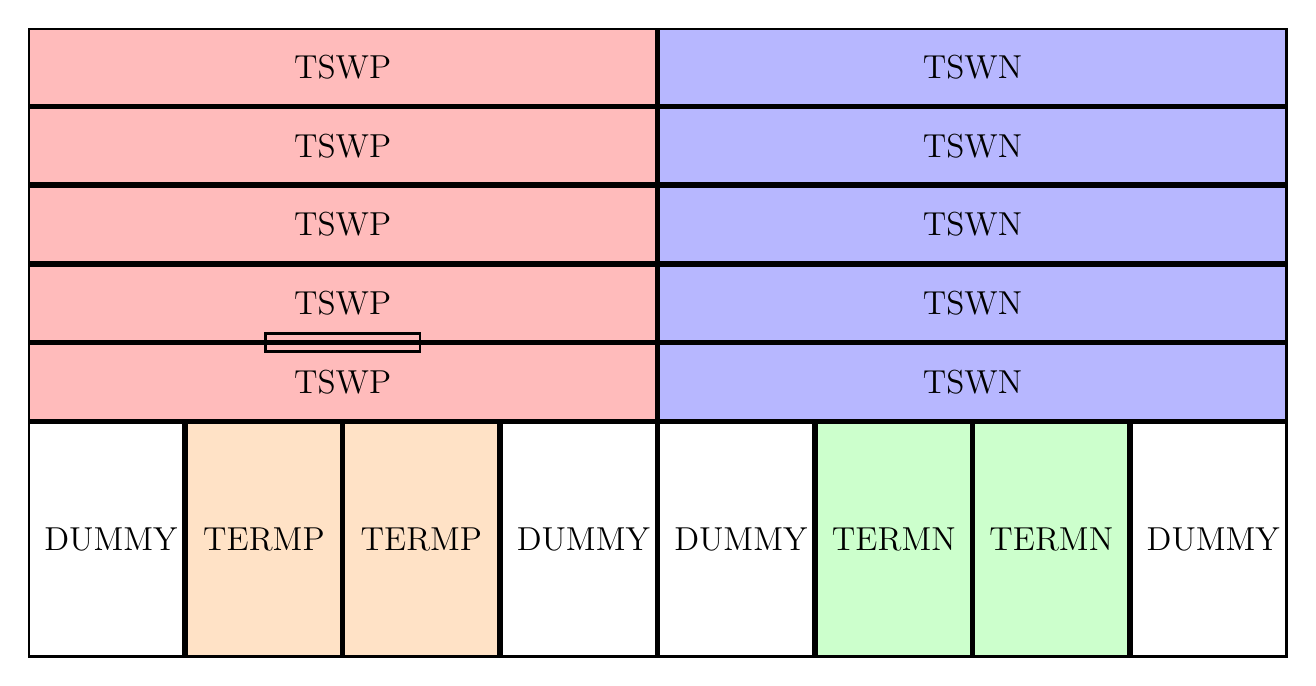
\begin{tikzpicture}[transform shape]
		% Paths, nodes and wires:
		\node[shape=rectangle, fill={rgb,255:red,255;green,187;blue,187}, draw, line width=1pt, minimum width=7.965cm, minimum height=0.965cm] at (-4, 6.5){} node[anchor=center, align=center, text width=7.577cm, inner sep=6pt] at (-4, 6.5){\large TSWP};
		\node[shape=rectangle, fill={rgb,255:red,255;green,187;blue,187}, draw, line width=1pt, minimum width=7.965cm, minimum height=0.965cm] at (-4, 5.5){} node[anchor=center, align=center, text width=7.577cm, inner sep=6pt] at (-4, 5.5){\large TSWP};
		\node[shape=rectangle, fill={rgb,255:red,255;green,187;blue,187}, draw, line width=1pt, minimum width=7.965cm, minimum height=0.965cm] at (-4, 4.5){} node[anchor=center, align=center, text width=7.577cm, inner sep=6pt] at (-4, 4.5){\large TSWP};
		\node[shape=rectangle, fill={rgb,255:red,255;green,187;blue,187}, draw, line width=1pt, minimum width=7.965cm, minimum height=0.965cm] at (-4, 3.5){} node[anchor=center, align=center, text width=7.577cm, inner sep=6pt] at (-4, 3.5){\large TSWP};
		\node[shape=rectangle, fill={rgb,255:red,183;green,183;blue,255}, draw, line width=1pt, minimum width=7.965cm, minimum height=0.965cm] at (4, 6.5){} node[anchor=center, align=center, text width=7.577cm, inner sep=6pt] at (4, 6.5){\large TSWN};
		\node[shape=rectangle, fill={rgb,255:red,183;green,183;blue,255}, draw, line width=1pt, minimum width=7.965cm, minimum height=0.965cm] at (4, 5.5){} node[anchor=center, align=center, text width=7.577cm, inner sep=6pt] at (4, 5.5){\large TSWN};
		\node[shape=rectangle, fill={rgb,255:red,183;green,183;blue,255}, draw, line width=1pt, minimum width=7.965cm, minimum height=0.965cm] at (4, 4.5){} node[anchor=center, align=center, text width=7.577cm, inner sep=6pt] at (4, 4.5){\large TSWN};
		\node[shape=rectangle, fill={rgb,255:red,183;green,183;blue,255}, draw, line width=1pt, minimum width=7.965cm, minimum height=0.965cm] at (4, 3.5){} node[anchor=center, align=center, text width=7.577cm, inner sep=6pt] at (4, 3.5){\large TSWN};
		\node[shape=rectangle, draw, line width=1pt, minimum width=1.965cm, minimum height=-0.035cm] at (-4, 4){};
		\node[shape=rectangle, fill={rgb,255:red,204;green,255;blue,204}, draw, line width=1pt, minimum width=1.965cm, minimum height=2.965cm] at (3, 1.5){} node[anchor=center, align=center, text width=1.577cm, inner sep=6pt] at (3, 1.5){\large TERMN};
		\node[shape=rectangle, fill={rgb,255:red,204;green,255;blue,204}, draw, line width=1pt, minimum width=1.965cm, minimum height=2.965cm] at (5, 1.5){} node[anchor=center, align=center, text width=1.577cm, inner sep=6pt] at (5, 1.5){\large TERMN};
		\node[shape=rectangle, draw, line width=1pt, minimum width=1.965cm, minimum height=2.965cm] at (7, 1.5){} node[anchor=center, align=center, text width=1.577cm, inner sep=6pt] at (7, 1.5){\large DUMMY};
		\node[shape=rectangle, draw, line width=1pt, minimum width=1.965cm, minimum height=2.965cm] at (1, 1.5){} node[anchor=center, align=center, text width=1.577cm, inner sep=6pt] at (1, 1.5){\large DUMMY};
		\node[shape=rectangle, fill={rgb,255:red,255;green,226;blue,198}, draw, line width=1pt, minimum width=1.965cm, minimum height=2.965cm] at (-5, 1.5){} node[anchor=center, align=center, text width=1.577cm, inner sep=6pt] at (-5, 1.5){\large TERMP};
		\node[shape=rectangle, fill={rgb,255:red,255;green,226;blue,198}, draw, line width=1pt, minimum width=1.965cm, minimum height=2.965cm] at (-3, 1.5){} node[anchor=center, align=center, text width=1.577cm, inner sep=6pt] at (-3, 1.5){\large TERMP};
		\node[shape=rectangle, draw, line width=1pt, minimum width=1.965cm, minimum height=2.965cm] at (-1, 1.5){} node[anchor=center, align=center, text width=1.577cm, inner sep=6pt] at (-1, 1.5){\large DUMMY};
		\node[shape=rectangle, draw, line width=1pt, minimum width=1.965cm, minimum height=2.965cm] at (-7, 1.5){} node[anchor=center, align=center, text width=1.577cm, inner sep=6pt] at (-7, 1.5){\large DUMMY};
		\node[shape=rectangle, fill={rgb,255:red,255;green,187;blue,187}, draw, line width=1pt, minimum width=7.965cm, minimum height=0.965cm] at (-4, 7.5){} node[anchor=center, align=center, text width=7.577cm, inner sep=6pt] at (-4, 7.5){\large TSWP};
		\node[shape=rectangle, fill={rgb,255:red,183;green,183;blue,255}, draw, line width=1pt, minimum width=7.965cm, minimum height=0.965cm] at (4, 7.5){} node[anchor=center, align=center, text width=7.577cm, inner sep=6pt] at (4, 7.5){\large TSWN};
	\end{tikzpicture}
	}
	\caption{PMOS devices and resistors floorplan}\label{fig:PMOS_floorplan}
\end{figure}

This part of the tap unit floorplan is located at the top of the standard cell, right above the differential pair and the differential output nets. This positioning was chosen to minimize the length of the routing between the termination devices and the differential output nets, which carries the highest current density among the output nets, making IR Drop and \ac{EM} concerns more relevant for these nets. Figure~\ref{fig:high_level_tap_unit_floorplan} shows a high-level representation of the tap unit floorplan, highlighting the relative positioning of the differential pair, current mirrors, termination and switching devices.

\begin{figure}
	\centering
	\resizebox{0.2\textwidth}{!}{
	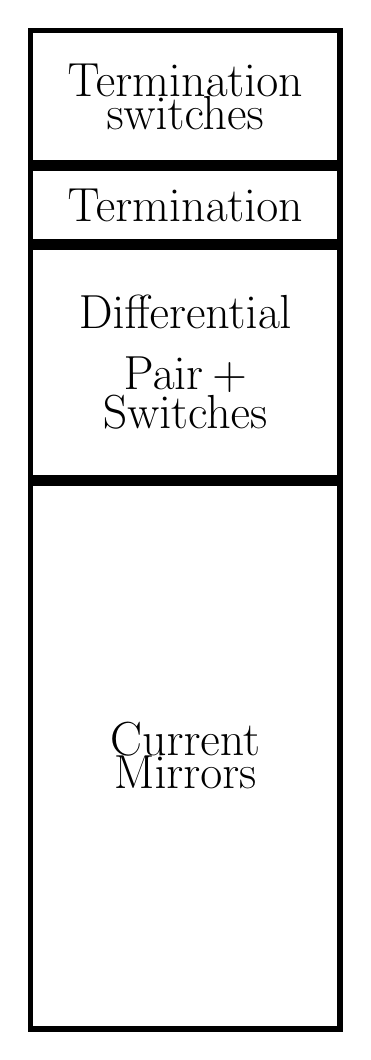
\begin{tikzpicture}[transform shape]
		% Paths, nodes and wires:
		\node[shape=rectangle, draw, line width=2pt, minimum width=3.929cm, minimum height=6.929cm] at (0, 3.5){} node[anchor=center, align=center, text width=3.506cm, inner sep=7pt] at (0, 3.5){\LARGE Current\\Mirrors};
		\node[shape=rectangle, draw, line width=2pt, minimum width=3.929cm, minimum height=2.929cm] at (0, 8.5){} node[anchor=center, align=center, text width=3.506cm, inner sep=7pt] at (0, 8.5){\LARGE Differential Pair +\\Switches};
		\node[shape=rectangle, draw, line width=2pt, minimum width=3.929cm, minimum height=1.679cm] at (0, 11.875){} node[anchor=center, align=center, text width=3.506cm, inner sep=7pt] at (0, 11.875){\LARGE Termination\\switches};
		\node[shape=rectangle, draw, line width=2pt, minimum width=3.929cm, minimum height=0.929cm] at (0, 10.5){} node[anchor=center, align=center, text width=3.506cm, inner sep=7pt] at (0, 10.5){\LARGE Termination};
	\end{tikzpicture}
	}
	\caption{High-level representation of the tap unit floorplan}\label{fig:high_level_tap_unit_floorplan}
\end{figure}

\subsection{Standard Cell Routing}\label{sec:standard_cell_routing}
% std cell has 6 enable nets for the current mirrors, 2 enable nets for the term devices, 2 differential input nets, 2 differential output nets, vref net for the mirrors, VDD and VSS nets
% descrever o placement de cada net, justificando nivel de metal usado, posição no layout, considerando diferença de potencial entre as nets (possiveis parasitas), crosstalk
% justificar width dos metais de acordo com a natureza de cada net (corrente, static/dynamic, sensibilidade a parasitas, etc), citando margens de EM e risco de IR drop

Following the floorplanning of the differential pair and current mirror bank, the routing of each basic tap unit standard cell was carried out with particular attention to the differing sensitivity of each signal type to parasitic effects, \ac{EM}, and crosstalk.

\subsubsection{Enable Signal Routing}

The nets carrying the enable signals for the current mirror and termination enabling devices are routed using polysilicon and the M1 metal layer, at the minimum width allowed by the technology. Since these signals are static during normal operation, and given the relatively short length of the associated routing paths, IR drop is not a significant concern for these nets; similarly, the low current density expected on these paths does not raise \ac{EM} concerns. Routing the enable nets on the lowest available layers frees up the higher metal layers for the differential pair and current mirror routing, which are considerably more sensitive to parasitic resistance and capacitance, and are subject to stricter \ac{EM} and IR drop requirements, as discussed further below.

Within the standard cell floorplan, the enable nets are routed predominantly along the top and bottom edges of the cell, while the differential input and output nets are routed through the middle of the cell. This placement was chosen with crosstalk in mind, in order to avoid coupling from the switching differential pair inadvertently toggling an enable signal to an incorrect level, and to minimize the parasitic loading introduced on the differential signal path by the fixed voltage levels of the nearby enable nets, which have their signal at either VDD or VSS, posing the highest voltage potential possible, during operation.

The enable pins themselves are placed along the bottom edge of the cell, with the exception of the termination enable pins, which partially overlap with the differential input and output nets. Since the differential input and output nets are routed mainly on the \ac{M4} layer, the termination enable nets connecting to the bottom of the cell use the \ac{M5} layer instead. This layer assignment was the result of routing congestion on layers M2 through \ac{M4} in the middle region of the cell. Among the remaining available layers, \ac{M5} resulted in the smallest and fewest overlapping regions with the other nets in the cell.

The current mirror bank enable nets are routed using M1 within the current mirror bank floorplan area itself, and \ac{M3} for the connections to the input ports located at the bottom of the cell. \ac{M3} was preferred over M2 for this purpose due to the heavy use of M1 already present within the current mirror bank floorplan area, resulting in less overlap with other nets when \ac{M3} is used instead. The only net that overlaps with the mirror bank enable nets is the reference voltage net, $V_{ref}$, which does so at eight points across the layout area. This overlap is not considered a significant concern, since the $V_{ref}$ signal is quasi-static, and combined with the static nature of the enable signals themselves, the resulting parasitic coupling capacitance is not expected to cause significant performance degradation, as both the $V_{ref}$ and enable signal levels are established at system start-up, well before the beginning of data transmission, providing sufficient time for these parasitic capacitances to fully charge.

\subsubsection{Reference Voltage Routing}

The $V_{ref}$ net is routed primarily using the \ac{M4} layer, since it must connect to adjacent tap unit cells as well as to the current mirror reference biasing circuit described in Section~\ref{sec:mirror_ref_dev}. Electromigration is not a significant concern for this net, since its sole function is to set the gate voltage of the current mirror devices, resulting in a low expected current density. Nonetheless, these nets were sized with a width 67\% larger than the minimum width allowed for the \ac{M4} layer, in order to account for the resistance of the routing path and its associated IR drop, and to keep the biasing voltage seen by the current mirror devices as close as possible to the reference value, minimizing the resulting error between the reference current and its mirrored copies.

\subsubsection{Differential Signal Routing}

The differential signal nets were the most critical nets in the standard cell, and consequently received the greatest attention during the planning and execution of the routing.

The first priority in routing these nets was to ensure that all differential nets of a given type, that is, the input pair or the output pair, were routed as symmetrically as possible with respect to one another, in order to avoid introducing timing skew between the two differential branches, consistent with the matching and symmetry principles discussed in Section~\ref{sec:routing_si}.

The second priority was to reduce parasitics on these nets while respecting the electromigration constraints of the metal layers used. To this end, the differential pair devices are implemented as four parallel sub-devices, each composed of ten fingers. As a result, the input signal nets, $D_p$ and $D_n$, are each split into ten parallel routing paths per sub-device, for a total of forty parallel paths connecting to the gate of each differential pair device.

The output nets, $TX_p$ and $TX_n$, are similarly split into five parallel routing paths per sub-device, connecting to the drain terminals of the current-steering devices, for a total of twenty parallel paths per output node. This parallelization means that the total current sunk by each tap is distributed across twenty parallel paths, which reduces the current density on each individual path and allows the routing metal width to be reduced accordingly, while still respecting the electromigration constraints imposed by the technology.

The differential nets are routed using the highest metal layers available for internal chip-level connections, \ac{M4} and \ac{M5}, in order to reduce parasitic coupling and crosstalk, avoid overlap with other nets in the cell, and avoid the routing congestion present on the lower metal layers. Although the differential routing was among the first aspects of the cell routing to be designed, its layout was defined with the routing requirements of the remaining, lower-priority nets on the lower metal layers already taken into consideration, in order to avoid conflicts later in the routing process.

\subsubsection{Electromigration Considerations}

From an \ac{EM} standpoint, the nets connecting the differential pair to the termination bank and to the current mirror bank were identified as the most critical in the design.

For the termination nets, the worst-case voltage drop considered across the termination network was 0.6~V, corresponding to the maximum single-ended output swing. Although the ideal resistor-only model of Section~\ref{sec:termination_control} would require approximately 20 parallel 1~k$\Omega$ elements to obtain a 50~$\Omega$ single-ended termination, this ideal relationship does not accurately represent the current distribution in the implemented termination bank. The effective impedance of an enabled termination branch is also affected by the switching device, whose simulated on-state resistance modifies the number of branches required to reach the target impedance.

For EM sizing, a value of approximately 10 simultaneously active termination paths was adopted as a conservative approximation of the implemented bank behaviour observed during circuit simulation. To avoid underestimating the current stress on the local termination routing, the total current associated with the maximum single-ended swing was conservatively assumed to be distributed among these 10 paths:

\begin{equation}
I_{\mathrm{path,EM}}
\approx
\frac{12~\mathrm{mA}}{10}
=
1.2~\mathrm{mA}.
\end{equation}

The resulting 1.2~mA value should therefore be interpreted as a conservative per-path current used for EM dimensioning, rather than as the exact current predicted by the ideal resistor-only model.

The width of the metal used to route these nets was chosen to keep the resulting current density within the \ac{EM} margins specified by the technology. Since the transmitted signal has a bit period of 100\,ps, the track width was sized using the peak current, $I_{peak}$, as the relevant \ac{EM} limit, rather than the \ac{RMS} current, $I_{RMS}$. This choice follows directly from the foundry's \ac{DRM}, which specifies that for any signal with a period shorter than a certain value, which is higher than the bit period of \SI{100}{\pico\second}, the \ac{EM} limit for the corresponding metal routing may be evaluated using $I_{peak}$ rather than $I_{RMS}$, which would otherwise impose a considerably tighter constraint on the required metal width.

The output nets, $TX_p$ and $TX_n$, correspond to the points in the layout where the currents associated with the transmitter termination and the receiver termination are combined, as discussed in Section~\ref{sec:tx_equalization}, and therefore exhibit the highest current density in the entire design. Since each tap unit is capable of sinking a maximum current of 1.2\,mA, the output metal tracks were sized to accommodate this current, in addition to satisfying the \ac{EM} limits imposed by the \ac{DRM}. Because these nets carry the same class of high-speed digital signal as the termination nets described above, the $I_{peak}$-based \ac{EM} limit was likewise used to determine the required \ac{M4} and \ac{M5} widths for the output nets.

Beyond these general current-density and \ac{EM} considerations, the routing in the immediate vicinity of the differential pair devices was designed specifically to avoid introducing parasitic Miller capacitance between the gate and drain terminals of the differential pair, which would otherwise degrade the performance of the driver.

%\subsubsection{Power Routing}

%\subsection{Current Mirrors Biasing Cell Layout}

%\subsection{Global Driver Layout}

%\subsubsection{Matching and Symmetry}

%The primary consideration guiding the layout of the driver is matching and symmetry between the two halves of the differential signal path. Any mismatch in parasitics or device characteristics between the positive and negative branches translates directly into duty-cycle distortion, common-mode-to-differential-mode conversion, and degraded equalization accuracy, all of which erode the timing and voltage margins of the transmitted eye. To minimize these effects, the differential pair of each basic tap unit is laid out using a common-centroid topology, ensuring that the two devices of the pair share the same geometric center and are therefore equally exposed to process gradients and systematic layout-induced mismatch.

%The current mirrors composing the current mirror bank of each stage are likewise matched using common centroid. This choice followed directly from floorplan constraints established earlier in the design: the differential pair and its associated switch devices were first floorplanned as RVT devices of a common gate length, and the resulting width of this block was used to constrain the floorplan of the current mirror bank. Given the number and gate length of the current mirror devices, an interdigitated layout was not feasible within the available area, and a common-centroid arrangement was adopted instead to achieve the required matching.

%To minimize the area overhead associated with matching, the non-active devices used purely for enabling and disabling elements of the current mirror and termination banks — namely the NMOS and PMOS switch devices — are reused as dummy devices for the matching structures, rather than introducing dedicated dummy devices solely for this purpose. This approach avoids the area penalty of adding non-functional dummy-only devices, since the switching devices already required by the circuit can serve a dual purpose.

%\subsubsection{Routing}

%The gates of all enabling and disabling switches within the current mirror and termination banks are routed using polysilicon rather than metal. Although polysilicon exhibits substantially higher sheet resistance than the available metal layers, this is not a concern in this context: the enable signals driving these switches are static, being configured once during system startup and held constant throughout normal operation, so the additional RC delay introduced by the poly routing has no impact on circuit performance. Routing these signals in poly instead of metal frees up metal layers for the differential pair and current mirror routing, which are considerably more sensitive to parasitic resistance and capacitance given their role in the high-speed signal path. Additionally, because the enable signals are low-current and quasi-static, the charge accumulated on the poly during processing is low, so process antenna effects are not expected to pose a reliability concern for this routing.

%\subsubsection{Substrate Noise and Latch-up}

%To mitigate substrate-borne disturbances — including minority-carrier injection from source/drain diffusions and substrate noise coupling — each group of devices sharing a common flavor is enclosed within a dedicated guard ring. Beyond suppressing substrate noise coupling, these guard rings also serve a reliability function, preventing the formation of parasitic low-impedance conduction paths between adjacent PMOS and NMOS structures that could otherwise trigger latch-up, a self-sustaining short-circuit condition capable of causing permanent device damage.

%\subsubsection{Electromigration and Routing Area}

%Electromigration constraints are taken into account throughout the routing of the driver. For nodes carrying high current density, such as the tail current and output signal paths, wire widths are sized to keep current density within the electromigration limits imposed by the technology. Conversely, for lower-current-density nets, routing area is deliberately minimized within the technology's Design Rule Manual (DRM), since these nets are not electromigration-critical, using minimum-width routing on lower metal layers avoids unnecessarily consuming wider or higher metal layers that would otherwise increase the overall layout area without providing any significant reliability benefit.

%\subsubsection{Modularity}

%The driver layout is partitioned into two main building blocks: the CML tap unit, comprising the differential pair, current mirror bank, and termination bank of a single tap; and the current mirror biasing block, which generates the reference currents used by the mirror banks. Both blocks are designed as standard cells following a modular, abuttable floorplan, such that CML tap unit cells can be placed directly adjacent to one another, or adjacent to the biasing and end cells. This modularity allows the number of tap units instantiated in the design — and, consequently, the equalization resolution, output strenght or number of FFE taps — to be modified by simply adding or removing abutted cells, without needing a redesign of the underlying layout.

%\subsubsection{Power Rails Routing}

%The routing of the power supply network is designed with particular attention to the active devices it feeds, aiming to minimize both IR drop and switching noise on supply-sensitive nodes. This is especially critical for the paths supplying the DATA input and the transmission output stages, where supply noise couples directly into the transmitted signal and degrades output jitter and voltage margins. To this end, connections from the power routing to the active devices are made directly on top of the devices themselves, minimizing the length and resistance of the connection between the supply network and the current-carrying transistors.

%\textbf{ADICIONAR FIG DO LAYOUT AOS ANEXOS E REFERENCIAR}

\begin{comment}
- Main considerations for the layout of the driver are matching and symmetry, to ensure that the differential signal is symmetrically affected by layout parasitics
- Non active devices used only for switching, like the NMOS and PMOS devices used for enbaling/disabling in the current mirror and terminations banks, are used also used as dummies in matching, in order to use as little area as possible, and to avoid the use of non active devices that are not used for matching, which would increase the area of the layout
- Differential pair is matched using common centroid
- Current mirrors are also matched using common centroid. This design choice was made because, after the floorplan of the differential pair and mirror switches (as dummies for the diff pair), that are the same flavor (RVT) and have the same gate length, the width of the diff pair floorplan block was used to constrain the current mirror floorplan, and, because of the number and length of the current mirrors, interdigitation would not be possible for the available area, so common centroid was used
- In order to save metal layers, all enabling/disabling switches have their gates connected using poly. Even though poly has a higher resistance than metal, the static nature of the enbale signal (which is set during the startup of the system, and does not change during operation) makes this a non issue, and the use of poly allows to save metal layers for the differential pair and current mirrors, which are more sensitive to parasitics. Also, since the enabling signal is low current, process antenna effect should not be an issue, since the charges accumulated in the poly is low
- To clean up substrate disturbances (like minority carrier injected from source diffusions and substrate coupling noise), each group of devices with similar flavor is surrounded by a guard ring
    - Guard rings prevents the formation of low-impedance, short-circuit pathways known as latch-up
- Electromigration is taken into account both for high current density routing, and to minimize the routing area of smaller density ones, in order to keep layout area as small as possible, and to avoid the use of larger metal layers for smaller density routing
- The layout is split into two main blocks: the CML tap unit (diff pair + current mirror bank + termination bank), and the current mirror biasing block. 
    - The layout follows a modular approach, where each CML tap unit standard cell can be abutted to the next tap or the current biasing cell, which allows for a flexible layout, where the number of taps can be changed without having to redesign the layout from scratch
- Power supply routing takes into consideration the active devices, and connections to these devices are done in a way to minimize IR drop and switching noise for critical signal paths, like the DATA input and Transmission output
    - Connection to the power routing is done on top of the active devices
\end{comment}

